% !Mode:: "TeX:UTF-8"
% !TEX program  = xelatex

% 模板名称:YangThesis
% 模板版本:V1.0
% 模板作者:JingXuan Yang
% 联系作者:yangjingxuan@stu.hit.edu.cn
% 模板来源:数模竞赛模板的二次开发
% 模板适用:普通课程论文,略作修改可用作毕业设计(论文)
% 模板编译:XeLaTeX,编译两次,两次,两次!!!
% 更新时间:4/14/2019
% 模板说明:本模板尽量把接口留在了类文件外面,但是顾名思义,模板即为
%                 部分样式的集合,有些样式是定义在类文件里面的,在外面无法
%                 修改。类文件中注释齐全,很多样式可以个性化定义,建议拥有
%                 一定LaTeX基础以后再尝试修改类文件(YangThesis.cls)。

% 本模板提供有、无封面两种选择
% 1、采用封面
% 模板默认采用封面
% no-math选项指不采用模板文件对数学符号字体的定义
% 可在settings.tex里设置数学符号字体

\documentclass[no-math]{YangThesis} 

% 2、去掉封面,添加<withoutpreface>选项
%\documentclass[no-math, withoutpreface]{YangThesis} 

% 导入配置文件settings.tex,
% 配置参数均存储在settings.tex文件中,
% 添加或修改均需在该文件中进行
% settings.tex
% YangTemplate.cls 的配置文件
% 采用<\input>放入主文档中,不可单独编译

% 设置bib管理的参考文献样式
% https://github.com/CTeX-orggbt7714-bibtex-style
% \bibliographystyle{elsarticle-num}

%\usepackage[numbers]{gbt7714}

% 设置bib管理的参考文献样式
% https://github.com/CTeX-orggbt7714-bibtex-style
% \usepackage[numbers]{gbt7714}
% 使用BibLatex的方法,再配合标准的2015文件
% https://github.com/hushidong/biblatex-gb7714-2015

%导言区开始:

%加载hyperref宏包, 使用超链接
%\usepackage[colorlinks=true,pdfstartview=FitH,linkcolor=blue,anchorcolor=violet,citecolor=magenta]{hyperref}
\usepackage[backend=biber,style=gb7714-2015]{biblatex}
%biblatex宏包的参考文献数据源加载方式
%\addbibresource[location=local]{ml.bib}
%封面预先生成一页,后来用smallpdf来merge,代码缩进,靠shift tab手动缩进Python代码
\usepackage{pdfpages}% 插入pdf文件
\usepackage[T1]{fontenc}
\usepackage{booktabs}
\usepackage{graphicx}
% 正文和数学字体均采用Times New Roman字体
% \usepackage{newtxtext, newtxmath}

% 只正文采用Times字体,数学公式保持默认字体
\usepackage{newtxtext}

\usepackage{float}
% 添加使用vscode 管理分支的测试代码
% 定制tikz流程图形状
\usepackage{tikz}
\usetikzlibrary{shapes.geometric, arrows,chains,snakes,backgrounds,calc}
% 开始
\tikzstyle{startstop} = [rectangle, rounded corners, minimum width = 2cm, minimum height=1cm,text centered, draw = black]
%矩形,加圆角
% 输入输出
\tikzstyle{io} = [trapezium, trapezium left angle=70, trapezium right angle=110, minimum width=2cm, minimum height=1cm, text centered, draw=black]
%平行四边形
% 过程
\tikzstyle{process} = [rectangle, minimum width=3cm, minimum height=1cm, text centered, draw=black]
% 判断
\tikzstyle{decision} = [diamond, aspect = 3, text centered, draw=black]
%菱形
% 箭头形式
\tikzstyle{arrow} = [->,>=stealth]

% 设置编号格式
\newcounter{rowno}
\numberwithin{equation}{section}
\numberwithin{figure}{section}
\numberwithin{table}{section}
\renewcommand{\thefigure}{\arabic{section}-\arabic{figure}}
\renewcommand{\thetable}{\arabic{section}-\arabic{table}}
\renewcommand{\theequation}{\arabic{section}-\arabic{equation}}

% 新数学命令
\newcommand\dif{\mathrm{d}}
\newcommand\no{\noindent}
\newcommand\dis{\displaystyle}
\newcommand\ls{\leqslant}
\newcommand\gs{\geqslant}

\newcommand\limit{\dis\lim\limits}
\newcommand\limn{\dis\lim\limits_{n\to\infty}}
\newcommand\limxz{\dis\lim\limits_{x\to0}}
\newcommand\limxi{\dis\lim\limits_{x\to\infty}}
\newcommand\limxpi{\dis\lim\limits_{x\to+\infty}}
\newcommand\limxni{\dis\lim\limits_{x\to-\infty}}

% 默认上限为无穷
\newcommand\sumnf{\dis\sum\limits_{n=1}^{\infty}}
\newcommand\sumnz{\dis\sum\limits_{n=0}^{\infty}}
\newcommand\sumkf{\dis\sum\limits_{k=1}^{\infty}}
\newcommand\sumkz{\dis\sum\limits_{k=0}^{\infty}}
\newcommand\sumifn{\dis\sum\limits_{i=1}^{n}}
\newcommand\sumizn{\dis\sum\limits_{i=0}^{n}}
\newcommand\sumkzn{\dis\sum\limits_{k=0}^n}
\newcommand\sumkfn{\dis\sum\limits_{k=1}^n}

\newcommand\pzx{\dis\frac{\partial z}{\partial x}}
\newcommand\pzy{\dis\frac{\partial z}{\partial y}}

\newcommand\pfx{\dis\frac{\partial f}{\partial x}}
\newcommand\pfy{\dis\frac{\partial f}{\partial x}}

\newcommand\pzxx{\dis\frac{\partial^2 z}{\partial x^2}}
\newcommand\pzxy{\dis\frac{\partial^2 z}{\partial x\partial y}}
\newcommand\pzyx{\dis\frac{\partial^2 z}{\partial y\partial x}}
\newcommand\pzyy{\dis\frac{\partial^2 z}{\partial y^2}}

\newcommand\pfxx{\dis\frac{\partial^2 f}{\partial x^2}}
\newcommand\pfxy{\dis\frac{\partial^2 f}{\partial x\partial y}}
\newcommand\pfyx{\dis\frac{\partial^2 f}{\partial y\partial x}}
\newcommand\pfyy{\dis\frac{\partial^2 f}{\partial y^2}}

\newcommand\intzi{\dis\int_{0}^{+\infty}}
\newcommand\intd{\dis\int}
\newcommand\intab{\dis\int_a^b}

\newcommand\mc{\mathbb{C}}
\newcommand\mr{\mathbb{R}}
\newcommand{\degree}{^\circ}

\newenvironment{mfrac}[2]%
{\raise0.5ex\hbox{$#1$}\! \left/ \! \lower0.5ex\hbox{$#2$}\right.}

% 定义新数学符号
\DeclareMathOperator{\sgn}{sgn}
\DeclareMathOperator{\arccot}{arccot}
\DeclareMathOperator{\arccosh}{arccosh}
\DeclareMathOperator{\arcsinh}{arcsinh}
\DeclareMathOperator{\arctanh}{arctanh}
\DeclareMathOperator{\arccoth}{arccoth}
\DeclareMathOperator{\grad}{\bf{grad}}
\DeclareMathOperator{\diag}{diag}
\DeclareMathOperator{\csign}{csign}

\usepackage{url}

% 自定义字号大小命令
% 修改18pt为想要的字号即可
\newcommand{\myfont}{\fontsize{18pt}{\baselineskip}\selectfont}

% 参考文献标号为上标
%newcommand{\upcite}[1]{\textsuperscript{\textsuperscript{\cite{#1}}}}

% 定制页眉页脚
\usepackage{fancyhdr}
\pagestyle{fancy}
% 页眉
\lhead{}
\chead{房价预测}
\rhead{}
% 页脚
\lfoot{}
\cfoot{-\thepage-}
\rfoot{}

% 页眉页脚单横线
%\renewcommand{\headrulewidth}{0.4pt}
%\renewcommand{\footrulewidth}{0pt}

% 页眉双横线
\newcommand{\makeheadrule}{%
\makebox[0pt][l]{\rule[0.2\baselineskip]{\headwidth}{1.3pt}}%
\rule[0.35\baselineskip]{\headwidth}{2.5pt}}
\renewcommand{\headrule}{%
{\if@fancyplain\let\headrulewidth\plainheadrulewidth\fi
\makeheadrule}}
\makeatother

% 设置脚注编号格式
\renewcommand{\thefootnote}{\fnsymbol{footnote}}



% 封面信息
% 论文类别
\papercategory{高级人工智能课程实验报告}
% 论文标题
\title{房价预测}

% 学校名称
\schoolname{南京航空航天大学}
% 学院名称
\departname{计算机科学与技术学院}
% 专业
\majorin{计算机技术}
% 班级
%\classnumber{中特社17班}
% 姓名
\authorname{林国瑞}
% 学号
\studentID{SF1916009}
% 教师
\teacher{徐敏,关东海}
% 日期
\dateinput{2019年12月15日}
\usepackage[breakable]{tcolorbox}
\usepackage{parskip} % Stop auto-indenting (to mimic markdown behaviour)

\usepackage{iftex}
\ifPDFTeX
\usepackage[T1]{fontenc}
\usepackage{mathpazo}
\else
\usepackage{fontspec}
\fi

% Basic figure setup, for now with no caption control since it's done
% automatically by Pandoc (which extracts ![](path) syntax from Markdown).
\usepackage{graphicx}
% Maintain compatibility with old templates. Remove in nbconvert 6.0
\let\Oldincludegraphics\includegraphics
% Ensure that by default, figures have no caption (until we provide a
% proper Figure object with a Caption API and a way to capture that
% in the conversion process - todo).
\usepackage{caption}
\DeclareCaptionFormat{nocaption}{}
\captionsetup{format=nocaption,aboveskip=0pt,belowskip=0pt}

\usepackage[Export]{adjustbox} % Used to constrain images to a maximum size
\adjustboxset{max size={0.9\linewidth}{0.9\paperheight}}
\usepackage{float}
\floatplacement{figure}{H} % forces figures to be placed at the correct location
\usepackage{xcolor} % Allow colors to be defined
\usepackage{enumerate} % Needed for markdown enumerations to work
\usepackage{geometry} % Used to adjust the document margins
\usepackage{amsmath} % Equations
\usepackage{amssymb} % Equations
\usepackage{textcomp} % defines textquotesingle
% Hack from http://tex.stackexchange.com/a/47451/13684:
\AtBeginDocument{%
	\def\PYZsq{\textquotesingle}% Upright quotes in Pygmentized code
}
\usepackage{upquote} % Upright quotes for verbatim code
\usepackage{eurosym} % defines \euro
%\usepackage[mathletters]{ucs} % Extended unicode (utf-8) support
\usepackage{fancyvrb} % verbatim replacement that allows latex
\usepackage{grffile} % extends the file name processing of package graphics 
% to support a larger range
\makeatletter % fix for grffile with XeLaTeX
\def\Gread@@xetex#1{%
	\IfFileExists{"\Gin@base".bb}%
	{\Gread@eps{\Gin@base.bb}}%
	{\Gread@@xetex@aux#1}%
}
\makeatother

% The hyperref package gives us a pdf with properly built
% internal navigation ('pdf bookmarks' for the table of contents,
% internal cross-reference links, web links for URLs, etc.)
\usepackage{hyperref}
% The default LaTeX title has an obnoxious amount of whitespace. By default,
% titling removes some of it. It also provides customization options.
\usepackage{titling}
\usepackage{longtable} % longtable support required by pandoc >1.10
\usepackage{booktabs}  % table support for pandoc > 1.12.2
\usepackage[inline]{enumitem} % IRkernel/repr support (it uses the enumerate* environment)
%\usepackage[normalem]{ulem} % ulem is needed to support strikethroughs (\sout)
% normalem makes italics be italics, not underlines
%\usepackage{mathrsfs}



% Colors for the hyperref package
\definecolor{urlcolor}{rgb}{0,.145,.698}
\definecolor{linkcolor}{rgb}{.71,0.21,0.01}
\definecolor{citecolor}{rgb}{.12,.54,.11}

% ANSI colors
\definecolor{ansi-black}{HTML}{3E424D}
\definecolor{ansi-black-intense}{HTML}{282C36}
\definecolor{ansi-red}{HTML}{E75C58}
\definecolor{ansi-red-intense}{HTML}{B22B31}
\definecolor{ansi-green}{HTML}{00A250}
\definecolor{ansi-green-intense}{HTML}{007427}
\definecolor{ansi-yellow}{HTML}{DDB62B}
\definecolor{ansi-yellow-intense}{HTML}{B27D12}
\definecolor{ansi-blue}{HTML}{208FFB}
\definecolor{ansi-blue-intense}{HTML}{0065CA}
\definecolor{ansi-magenta}{HTML}{D160C4}
\definecolor{ansi-magenta-intense}{HTML}{A03196}
\definecolor{ansi-cyan}{HTML}{60C6C8}
\definecolor{ansi-cyan-intense}{HTML}{258F8F}
\definecolor{ansi-white}{HTML}{C5C1B4}
\definecolor{ansi-white-intense}{HTML}{A1A6B2}
\definecolor{ansi-default-inverse-fg}{HTML}{FFFFFF}
\definecolor{ansi-default-inverse-bg}{HTML}{000000}

% commands and environments needed by pandoc snippets
% extracted from the output of `pandoc -s`
\providecommand{\tightlist}{%
	\setlength{\itemsep}{0pt}\setlength{\parskip}{0pt}}
\DefineVerbatimEnvironment{Highlighting}{Verbatim}{commandchars=\\\{\}}
% Add ',fontsize=\small' for more characters per line
\newenvironment{Shaded}{}{}
\newcommand{\KeywordTok}[1]{\textcolor[rgb]{0.00,0.44,0.13}{\textbf{{#1}}}}
\newcommand{\DataTypeTok}[1]{\textcolor[rgb]{0.56,0.13,0.00}{{#1}}}
\newcommand{\DecValTok}[1]{\textcolor[rgb]{0.25,0.63,0.44}{{#1}}}
\newcommand{\BaseNTok}[1]{\textcolor[rgb]{0.25,0.63,0.44}{{#1}}}
\newcommand{\FloatTok}[1]{\textcolor[rgb]{0.25,0.63,0.44}{{#1}}}
\newcommand{\CharTok}[1]{\textcolor[rgb]{0.25,0.44,0.63}{{#1}}}
\newcommand{\StringTok}[1]{\textcolor[rgb]{0.25,0.44,0.63}{{#1}}}
\newcommand{\CommentTok}[1]{\textcolor[rgb]{0.38,0.63,0.69}{\textit{{#1}}}}
\newcommand{\OtherTok}[1]{\textcolor[rgb]{0.00,0.44,0.13}{{#1}}}
\newcommand{\AlertTok}[1]{\textcolor[rgb]{1.00,0.00,0.00}{\textbf{{#1}}}}
\newcommand{\FunctionTok}[1]{\textcolor[rgb]{0.02,0.16,0.49}{{#1}}}
\newcommand{\RegionMarkerTok}[1]{{#1}}
\newcommand{\ErrorTok}[1]{\textcolor[rgb]{1.00,0.00,0.00}{\textbf{{#1}}}}
\newcommand{\NormalTok}[1]{{#1}}

% Additional commands for more recent versions of Pandoc
\newcommand{\ConstantTok}[1]{\textcolor[rgb]{0.53,0.00,0.00}{{#1}}}
\newcommand{\SpecialCharTok}[1]{\textcolor[rgb]{0.25,0.44,0.63}{{#1}}}
\newcommand{\VerbatimStringTok}[1]{\textcolor[rgb]{0.25,0.44,0.63}{{#1}}}
\newcommand{\SpecialStringTok}[1]{\textcolor[rgb]{0.73,0.40,0.53}{{#1}}}
\newcommand{\ImportTok}[1]{{#1}}
\newcommand{\DocumentationTok}[1]{\textcolor[rgb]{0.73,0.13,0.13}{\textit{{#1}}}}
\newcommand{\AnnotationTok}[1]{\textcolor[rgb]{0.38,0.63,0.69}{\textbf{\textit{{#1}}}}}
\newcommand{\CommentVarTok}[1]{\textcolor[rgb]{0.38,0.63,0.69}{\textbf{\textit{{#1}}}}}
\newcommand{\VariableTok}[1]{\textcolor[rgb]{0.10,0.09,0.49}{{#1}}}
\newcommand{\ControlFlowTok}[1]{\textcolor[rgb]{0.00,0.44,0.13}{\textbf{{#1}}}}
\newcommand{\OperatorTok}[1]{\textcolor[rgb]{0.40,0.40,0.40}{{#1}}}
\newcommand{\BuiltInTok}[1]{{#1}}
\newcommand{\ExtensionTok}[1]{{#1}}
\newcommand{\PreprocessorTok}[1]{\textcolor[rgb]{0.74,0.48,0.00}{{#1}}}
\newcommand{\AttributeTok}[1]{\textcolor[rgb]{0.49,0.56,0.16}{{#1}}}
\newcommand{\InformationTok}[1]{\textcolor[rgb]{0.38,0.63,0.69}{\textbf{\textit{{#1}}}}}
\newcommand{\WarningTok}[1]{\textcolor[rgb]{0.38,0.63,0.69}{\textbf{\textit{{#1}}}}}


% Define a nice break command that doesn't care if a line doesn't already
% exist.
\def\br{\hspace*{\fill} \\* }
% Math Jax compatibility definitions
\def\gt{>}
\def\lt{<}
\let\Oldtex\TeX
\let\Oldlatex\LaTeX
\renewcommand{\TeX}{\textrm{\Oldtex}}
\renewcommand{\LaTeX}{\textrm{\Oldlatex}}
% Document parameters
% Document title
%\title{house\_price\_csdn}





% Pygments definitions
\makeatletter
\def\PY@reset{\let\PY@it=\relax \let\PY@bf=\relax%
	\let\PY@ul=\relax \let\PY@tc=\relax%
	\let\PY@bc=\relax \let\PY@ff=\relax}
\def\PY@tok#1{\csname PY@tok@#1\endcsname}
\def\PY@toks#1+{\ifx\relax#1\empty\else%
	\PY@tok{#1}\expandafter\PY@toks\fi}
\def\PY@do#1{\PY@bc{\PY@tc{\PY@ul{%
				\PY@it{\PY@bf{\PY@ff{#1}}}}}}}
\def\PY#1#2{\PY@reset\PY@toks#1+\relax+\PY@do{#2}}

\expandafter\def\csname PY@tok@w\endcsname{\def\PY@tc##1{\textcolor[rgb]{0.73,0.73,0.73}{##1}}}
\expandafter\def\csname PY@tok@c\endcsname{\let\PY@it=\textit\def\PY@tc##1{\textcolor[rgb]{0.25,0.50,0.50}{##1}}}
\expandafter\def\csname PY@tok@cp\endcsname{\def\PY@tc##1{\textcolor[rgb]{0.74,0.48,0.00}{##1}}}
\expandafter\def\csname PY@tok@k\endcsname{\let\PY@bf=\textbf\def\PY@tc##1{\textcolor[rgb]{0.00,0.50,0.00}{##1}}}
\expandafter\def\csname PY@tok@kp\endcsname{\def\PY@tc##1{\textcolor[rgb]{0.00,0.50,0.00}{##1}}}
\expandafter\def\csname PY@tok@kt\endcsname{\def\PY@tc##1{\textcolor[rgb]{0.69,0.00,0.25}{##1}}}
\expandafter\def\csname PY@tok@o\endcsname{\def\PY@tc##1{\textcolor[rgb]{0.40,0.40,0.40}{##1}}}
\expandafter\def\csname PY@tok@ow\endcsname{\let\PY@bf=\textbf\def\PY@tc##1{\textcolor[rgb]{0.67,0.13,1.00}{##1}}}
\expandafter\def\csname PY@tok@nb\endcsname{\def\PY@tc##1{\textcolor[rgb]{0.00,0.50,0.00}{##1}}}
\expandafter\def\csname PY@tok@nf\endcsname{\def\PY@tc##1{\textcolor[rgb]{0.00,0.00,1.00}{##1}}}
\expandafter\def\csname PY@tok@nc\endcsname{\let\PY@bf=\textbf\def\PY@tc##1{\textcolor[rgb]{0.00,0.00,1.00}{##1}}}
\expandafter\def\csname PY@tok@nn\endcsname{\let\PY@bf=\textbf\def\PY@tc##1{\textcolor[rgb]{0.00,0.00,1.00}{##1}}}
\expandafter\def\csname PY@tok@ne\endcsname{\let\PY@bf=\textbf\def\PY@tc##1{\textcolor[rgb]{0.82,0.25,0.23}{##1}}}
\expandafter\def\csname PY@tok@nv\endcsname{\def\PY@tc##1{\textcolor[rgb]{0.10,0.09,0.49}{##1}}}
\expandafter\def\csname PY@tok@no\endcsname{\def\PY@tc##1{\textcolor[rgb]{0.53,0.00,0.00}{##1}}}
\expandafter\def\csname PY@tok@nl\endcsname{\def\PY@tc##1{\textcolor[rgb]{0.63,0.63,0.00}{##1}}}
\expandafter\def\csname PY@tok@ni\endcsname{\let\PY@bf=\textbf\def\PY@tc##1{\textcolor[rgb]{0.60,0.60,0.60}{##1}}}
\expandafter\def\csname PY@tok@na\endcsname{\def\PY@tc##1{\textcolor[rgb]{0.49,0.56,0.16}{##1}}}
\expandafter\def\csname PY@tok@nt\endcsname{\let\PY@bf=\textbf\def\PY@tc##1{\textcolor[rgb]{0.00,0.50,0.00}{##1}}}
\expandafter\def\csname PY@tok@nd\endcsname{\def\PY@tc##1{\textcolor[rgb]{0.67,0.13,1.00}{##1}}}
\expandafter\def\csname PY@tok@s\endcsname{\def\PY@tc##1{\textcolor[rgb]{0.73,0.13,0.13}{##1}}}
\expandafter\def\csname PY@tok@sd\endcsname{\let\PY@it=\textit\def\PY@tc##1{\textcolor[rgb]{0.73,0.13,0.13}{##1}}}
\expandafter\def\csname PY@tok@si\endcsname{\let\PY@bf=\textbf\def\PY@tc##1{\textcolor[rgb]{0.73,0.40,0.53}{##1}}}
\expandafter\def\csname PY@tok@se\endcsname{\let\PY@bf=\textbf\def\PY@tc##1{\textcolor[rgb]{0.73,0.40,0.13}{##1}}}
\expandafter\def\csname PY@tok@sr\endcsname{\def\PY@tc##1{\textcolor[rgb]{0.73,0.40,0.53}{##1}}}
\expandafter\def\csname PY@tok@ss\endcsname{\def\PY@tc##1{\textcolor[rgb]{0.10,0.09,0.49}{##1}}}
\expandafter\def\csname PY@tok@sx\endcsname{\def\PY@tc##1{\textcolor[rgb]{0.00,0.50,0.00}{##1}}}
\expandafter\def\csname PY@tok@m\endcsname{\def\PY@tc##1{\textcolor[rgb]{0.40,0.40,0.40}{##1}}}
\expandafter\def\csname PY@tok@gh\endcsname{\let\PY@bf=\textbf\def\PY@tc##1{\textcolor[rgb]{0.00,0.00,0.50}{##1}}}
\expandafter\def\csname PY@tok@gu\endcsname{\let\PY@bf=\textbf\def\PY@tc##1{\textcolor[rgb]{0.50,0.00,0.50}{##1}}}
\expandafter\def\csname PY@tok@gd\endcsname{\def\PY@tc##1{\textcolor[rgb]{0.63,0.00,0.00}{##1}}}
\expandafter\def\csname PY@tok@gi\endcsname{\def\PY@tc##1{\textcolor[rgb]{0.00,0.63,0.00}{##1}}}
\expandafter\def\csname PY@tok@gr\endcsname{\def\PY@tc##1{\textcolor[rgb]{1.00,0.00,0.00}{##1}}}
\expandafter\def\csname PY@tok@ge\endcsname{\let\PY@it=\textit}
\expandafter\def\csname PY@tok@gs\endcsname{\let\PY@bf=\textbf}
\expandafter\def\csname PY@tok@gp\endcsname{\let\PY@bf=\textbf\def\PY@tc##1{\textcolor[rgb]{0.00,0.00,0.50}{##1}}}
\expandafter\def\csname PY@tok@go\endcsname{\def\PY@tc##1{\textcolor[rgb]{0.53,0.53,0.53}{##1}}}
\expandafter\def\csname PY@tok@gt\endcsname{\def\PY@tc##1{\textcolor[rgb]{0.00,0.27,0.87}{##1}}}
\expandafter\def\csname PY@tok@err\endcsname{\def\PY@bc##1{\setlength{\fboxsep}{0pt}\fcolorbox[rgb]{1.00,0.00,0.00}{1,1,1}{\strut ##1}}}
\expandafter\def\csname PY@tok@kc\endcsname{\let\PY@bf=\textbf\def\PY@tc##1{\textcolor[rgb]{0.00,0.50,0.00}{##1}}}
\expandafter\def\csname PY@tok@kd\endcsname{\let\PY@bf=\textbf\def\PY@tc##1{\textcolor[rgb]{0.00,0.50,0.00}{##1}}}
\expandafter\def\csname PY@tok@kn\endcsname{\let\PY@bf=\textbf\def\PY@tc##1{\textcolor[rgb]{0.00,0.50,0.00}{##1}}}
\expandafter\def\csname PY@tok@kr\endcsname{\let\PY@bf=\textbf\def\PY@tc##1{\textcolor[rgb]{0.00,0.50,0.00}{##1}}}
\expandafter\def\csname PY@tok@bp\endcsname{\def\PY@tc##1{\textcolor[rgb]{0.00,0.50,0.00}{##1}}}
\expandafter\def\csname PY@tok@fm\endcsname{\def\PY@tc##1{\textcolor[rgb]{0.00,0.00,1.00}{##1}}}
\expandafter\def\csname PY@tok@vc\endcsname{\def\PY@tc##1{\textcolor[rgb]{0.10,0.09,0.49}{##1}}}
\expandafter\def\csname PY@tok@vg\endcsname{\def\PY@tc##1{\textcolor[rgb]{0.10,0.09,0.49}{##1}}}
\expandafter\def\csname PY@tok@vi\endcsname{\def\PY@tc##1{\textcolor[rgb]{0.10,0.09,0.49}{##1}}}
\expandafter\def\csname PY@tok@vm\endcsname{\def\PY@tc##1{\textcolor[rgb]{0.10,0.09,0.49}{##1}}}
\expandafter\def\csname PY@tok@sa\endcsname{\def\PY@tc##1{\textcolor[rgb]{0.73,0.13,0.13}{##1}}}
\expandafter\def\csname PY@tok@sb\endcsname{\def\PY@tc##1{\textcolor[rgb]{0.73,0.13,0.13}{##1}}}
\expandafter\def\csname PY@tok@sc\endcsname{\def\PY@tc##1{\textcolor[rgb]{0.73,0.13,0.13}{##1}}}
\expandafter\def\csname PY@tok@dl\endcsname{\def\PY@tc##1{\textcolor[rgb]{0.73,0.13,0.13}{##1}}}
\expandafter\def\csname PY@tok@s2\endcsname{\def\PY@tc##1{\textcolor[rgb]{0.73,0.13,0.13}{##1}}}
\expandafter\def\csname PY@tok@sh\endcsname{\def\PY@tc##1{\textcolor[rgb]{0.73,0.13,0.13}{##1}}}
\expandafter\def\csname PY@tok@s1\endcsname{\def\PY@tc##1{\textcolor[rgb]{0.73,0.13,0.13}{##1}}}
\expandafter\def\csname PY@tok@mb\endcsname{\def\PY@tc##1{\textcolor[rgb]{0.40,0.40,0.40}{##1}}}
\expandafter\def\csname PY@tok@mf\endcsname{\def\PY@tc##1{\textcolor[rgb]{0.40,0.40,0.40}{##1}}}
\expandafter\def\csname PY@tok@mh\endcsname{\def\PY@tc##1{\textcolor[rgb]{0.40,0.40,0.40}{##1}}}
\expandafter\def\csname PY@tok@mi\endcsname{\def\PY@tc##1{\textcolor[rgb]{0.40,0.40,0.40}{##1}}}
\expandafter\def\csname PY@tok@il\endcsname{\def\PY@tc##1{\textcolor[rgb]{0.40,0.40,0.40}{##1}}}
\expandafter\def\csname PY@tok@mo\endcsname{\def\PY@tc##1{\textcolor[rgb]{0.40,0.40,0.40}{##1}}}
\expandafter\def\csname PY@tok@ch\endcsname{\let\PY@it=\textit\def\PY@tc##1{\textcolor[rgb]{0.25,0.50,0.50}{##1}}}
\expandafter\def\csname PY@tok@cm\endcsname{\let\PY@it=\textit\def\PY@tc##1{\textcolor[rgb]{0.25,0.50,0.50}{##1}}}
\expandafter\def\csname PY@tok@cpf\endcsname{\let\PY@it=\textit\def\PY@tc##1{\textcolor[rgb]{0.25,0.50,0.50}{##1}}}
\expandafter\def\csname PY@tok@c1\endcsname{\let\PY@it=\textit\def\PY@tc##1{\textcolor[rgb]{0.25,0.50,0.50}{##1}}}
\expandafter\def\csname PY@tok@cs\endcsname{\let\PY@it=\textit\def\PY@tc##1{\textcolor[rgb]{0.25,0.50,0.50}{##1}}}

\def\PYZbs{\char`\\}
\def\PYZus{\char`\_}
\def\PYZob{\char`\{}
\def\PYZcb{\char`\}}
\def\PYZca{\char`\^}
\def\PYZam{\char`\&}
\def\PYZlt{\char`\<}
\def\PYZgt{\char`\>}
\def\PYZsh{\char`\#}
\def\PYZpc{\char`\%}
\def\PYZdl{\char`\$}
\def\PYZhy{\char`\-}
\def\PYZsq{\char`\'}
\def\PYZdq{\char`\"}
\def\PYZti{\char`\~}
% for compatibility with earlier versions
\def\PYZat{@}
\def\PYZlb{[}
\def\PYZrb{]}
\makeatother


% For linebreaks inside Verbatim environment from package fancyvrb. 
\makeatletter
\newbox\Wrappedcontinuationbox 
\newbox\Wrappedvisiblespacebox 
\newcommand*\Wrappedvisiblespace {\textcolor{red}{\textvisiblespace}} 
\newcommand*\Wrappedcontinuationsymbol {\textcolor{red}{\llap{\tiny$\m@th\hookrightarrow$}}} 
\newcommand*\Wrappedcontinuationindent {3ex } 
\newcommand*\Wrappedafterbreak {\kern\Wrappedcontinuationindent\copy\Wrappedcontinuationbox} 
% Take advantage of the already applied Pygments mark-up to insert 
% potential linebreaks for TeX processing. 
%        {, <, #, %, $, ' and ": go to next line. 
%        _, }, ^, &, >, - and ~: stay at end of broken line. 
% Use of \textquotesingle for straight quote. 
\newcommand*\Wrappedbreaksatspecials {% 
	\def\PYGZus{\discretionary{\char`\_}{\Wrappedafterbreak}{\char`\_}}% 
	\def\PYGZob{\discretionary{}{\Wrappedafterbreak\char`\{}{\char`\{}}% 
	\def\PYGZcb{\discretionary{\char`\}}{\Wrappedafterbreak}{\char`\}}}% 
	\def\PYGZca{\discretionary{\char`\^}{\Wrappedafterbreak}{\char`\^}}% 
	\def\PYGZam{\discretionary{\char`\&}{\Wrappedafterbreak}{\char`\&}}% 
	\def\PYGZlt{\discretionary{}{\Wrappedafterbreak\char`\<}{\char`\<}}% 
	\def\PYGZgt{\discretionary{\char`\>}{\Wrappedafterbreak}{\char`\>}}% 
	\def\PYGZsh{\discretionary{}{\Wrappedafterbreak\char`\#}{\char`\#}}% 
	\def\PYGZpc{\discretionary{}{\Wrappedafterbreak\char`\%}{\char`\%}}% 
	\def\PYGZdl{\discretionary{}{\Wrappedafterbreak\char`\$}{\char`\$}}% 
	\def\PYGZhy{\discretionary{\char`\-}{\Wrappedafterbreak}{\char`\-}}% 
	\def\PYGZsq{\discretionary{}{\Wrappedafterbreak\textquotesingle}{\textquotesingle}}% 
	\def\PYGZdq{\discretionary{}{\Wrappedafterbreak\char`\"}{\char`\"}}% 
	\def\PYGZti{\discretionary{\char`\~}{\Wrappedafterbreak}{\char`\~}}% 
} 
% Some characters . , ; ? ! / are not pygmentized. 
% This macro makes them "active" and they will insert potential linebreaks 
\newcommand*\Wrappedbreaksatpunct {% 
	\lccode`\~`\.\lowercase{\def~}{\discretionary{\hbox{\char`\.}}{\Wrappedafterbreak}{\hbox{\char`\.}}}% 
	\lccode`\~`\,\lowercase{\def~}{\discretionary{\hbox{\char`\,}}{\Wrappedafterbreak}{\hbox{\char`\,}}}% 
	\lccode`\~`\;\lowercase{\def~}{\discretionary{\hbox{\char`\;}}{\Wrappedafterbreak}{\hbox{\char`\;}}}% 
	\lccode`\~`\:\lowercase{\def~}{\discretionary{\hbox{\char`\:}}{\Wrappedafterbreak}{\hbox{\char`\:}}}% 
	\lccode`\~`\?\lowercase{\def~}{\discretionary{\hbox{\char`\?}}{\Wrappedafterbreak}{\hbox{\char`\?}}}% 
	\lccode`\~`\!\lowercase{\def~}{\discretionary{\hbox{\char`\!}}{\Wrappedafterbreak}{\hbox{\char`\!}}}% 
	\lccode`\~`\/\lowercase{\def~}{\discretionary{\hbox{\char`\/}}{\Wrappedafterbreak}{\hbox{\char`\/}}}% 
	\catcode`\.\active
	\catcode`\,\active 
	\catcode`\;\active
	\catcode`\:\active
	\catcode`\?\active
	\catcode`\!\active
	\catcode`\/\active 
	\lccode`\~`\~ 	
}
\makeatother

\let\OriginalVerbatim=\Verbatim
\makeatletter
\renewcommand{\Verbatim}[1][1]{%
	%\parskip\z@skip
	\sbox\Wrappedcontinuationbox {\Wrappedcontinuationsymbol}%
	\sbox\Wrappedvisiblespacebox {\FV@SetupFont\Wrappedvisiblespace}%
	\def\FancyVerbFormatLine ##1{\hsize\linewidth
		\vtop{\raggedright\hyphenpenalty\z@\exhyphenpenalty\z@
			\doublehyphendemerits\z@\finalhyphendemerits\z@
			\strut ##1\strut}%
	}%
	% If the linebreak is at a space, the latter will be displayed as visible
	% space at end of first line, and a continuation symbol starts next line.
	% Stretch/shrink are however usually zero for typewriter font.
	\def\FV@Space {%
		\nobreak\hskip\z@ plus\fontdimen3\font minus\fontdimen4\font
		\discretionary{\copy\Wrappedvisiblespacebox}{\Wrappedafterbreak}
		{\kern\fontdimen2\font}%
	}%
	
	% Allow breaks at special characters using \PYG... macros.
	\Wrappedbreaksatspecials
	% Breaks at punctuation characters . , ; ? ! and / need catcode=\active 	
	\OriginalVerbatim[#1,codes*=\Wrappedbreaksatpunct]%
}
\makeatother

% Exact colors from NB
\definecolor{incolor}{HTML}{303F9F}
\definecolor{outcolor}{HTML}{D84315}
\definecolor{cellborder}{HTML}{CFCFCF}
\definecolor{cellbackground}{HTML}{F7F7F7}

% prompt
\makeatletter
\newcommand{\boxspacing}{\kern\kvtcb@left@rule\kern\kvtcb@boxsep}
\makeatother
\newcommand{\prompt}[4]{
	\ttfamily\llap{{\color{#2}[#3]:\hspace{3pt}#4}}\vspace{-\baselineskip}
}



% Prevent overflowing lines due to hard-to-break entities
\sloppy 
% Setup hyperref package
\hypersetup{
	breaklinks=true,  % so long urls are correctly broken across lines
	colorlinks=true,
	urlcolor=urlcolor,
	linkcolor=linkcolor,
	citecolor=citecolor,
}
% Slightly bigger margins than the latex defaults

\geometry{verbose,tmargin=1in,bmargin=1in,lmargin=1in,rmargin=1in}
%%%=====================%%%
% 开始写文章
\begin{document}
	
%\includepdfmerge{templates-face.pdf,1}
% 生成标题
\maketitle

% 页码从1开始计数
\setcounter{page}{1}
% 页码采用罗马数字格式
\pagenumbering{Roman}

\vspace{-1.3cm}

% 生成目录
\tableofcontents
% 将目录添加到目录中
%\addcontentsline{toc}{section}{目\,\,录}


% 分页,撰写正文
\clearpage
% 调整标题与上边的距离
\vspace{-1cm}
% 第1章的标题
\section{任务介绍}
% 关于论文的主题,基本上就是人工智能和伪科学二选一了,可是,伪科学,迷信,这些内容也已经有不少好的材料了。这种人文学科的问题可能就是值得发表的东西不多吧。何况已发表的也就是那个样子。不容易做出成果来。基本上,我总结一下看到的几篇网页就行了吧。
	
% 基本上所有搜集材料的过程结束了,目前不再在网上找阅读材料了,已经足够多了。

% 页码从1开始计数
\setcounter{page}{1}
% 页码格式采用阿拉伯数字
\pagenumbering{arabic}

Kaggle 是一个数据科学竞赛的平台。本次实验任务就是House Prices: Advanced Regression Techniques,一个房价预测的任务。
参加 kaggle 最简单的流程就是:

第一步:在 Data 里面下载三个数据集,最基本的就是上面提到的三个文件,有些比赛会有附加的数据描述文件等。

第二步:自己在线下分析,建模,调参,把用 test 数据集预测好的结果,按照 sample\_submission 的格式输出到 csv 文件中。

第三步:点击蓝色按钮 ’Submit Predictions’ ,把 csv 文件拖拽进去,然后系统就会加载并检验结果,稍等片刻后就会在 Leaderboard 上显示当前结果所在的排名位置。

使用Anaconda下的Jupyter notebook,用到了一些流行的第三方包。 
% 正文内容,注意LaTeX分段有两种方法,直接空一行或者使用<\par>
% 默认首行缩进,不需要在代码编辑区手动敲空格

% 需手动分页,为实现分页与不分页均可
% \newpage

% Create LaTeX tables online  http://www.tablesgenerator.com/#
% 这个网站比较神奇,竟然还有文本格式的表格生成,不过从使用角度讲,markdown语法太好用了,估计平常用的格式就是markdown,今天认识到了,日常的wps可以用来画图,可以用来画自己需要的示意图。通过表格的方法,画出时间线图,既能示意,效率也很高。比琢磨半天的xmind清晰明了多了。
% Please add the following required packages to your document preamble:
% \usepackage{booktabs}
% \usepackage{graphicx}
 \hypertarget{ux6570ux636eux96c6ux6982ux89c8}{%
	\section{数据集概览}\label{ux6570ux636eux96c6ux6982ux89c8}}

导入相关Python包:

\begin{tcolorbox}[breakable, size=fbox, boxrule=1pt, pad at break*=1mm,colback=cellbackground, colframe=cellborder]
	\prompt{In}{incolor}{1}{\boxspacing}
	\begin{Verbatim}[commandchars=\\\{\}]
\PY{c+c1}{\PYZsh{}import some necessary librairies}
	
\PY{k+kn}{import} \PY{n+nn}{numpy} \PY{k}{as} \PY{n+nn}{np} \PY{c+c1}{\PYZsh{} linear algebra}
\PY{k+kn}{import} \PY{n+nn}{pandas} \PY{k}{as} \PY{n+nn}{pd} \PY{c+c1}{\PYZsh{} data processing, CSV file I/O (e.g. pd.read\PYZus{}csv)}
\PY{o}{\PYZpc{}}\PY{k}{matplotlib} inline
\PY{k+kn}{import} \PY{n+nn}{matplotlib}\PY{n+nn}{.}\PY{n+nn}{pyplot} \PY{k}{as} \PY{n+nn}{plt}  \PY{c+c1}{\PYZsh{} Matlab\PYZhy{}style plotting}
\PY{k+kn}{import} \PY{n+nn}{seaborn} \PY{k}{as} \PY{n+nn}{sns}
\PY{n}{color} \PY{o}{=} \PY{n}{sns}\PY{o}{.}\PY{n}{color\PYZus{}palette}\PY{p}{(}\PY{p}{)}
\PY{n}{sns}\PY{o}{.}\PY{n}{set\PYZus{}style}\PY{p}{(}\PY{l+s+s1}{\PYZsq{}}\PY{l+s+s1}{darkgrid}\PY{l+s+s1}{\PYZsq{}}\PY{p}{)}
\PY{k+kn}{import} \PY{n+nn}{warnings}
\PY{k}{def} \PY{n+nf}{ignore\PYZus{}warn}\PY{p}{(}\PY{o}{*}\PY{n}{args}\PY{p}{,} \PY{o}{*}\PY{o}{*}\PY{n}{kwargs}\PY{p}{)}\PY{p}{:}
\PY{k}{pass}
\PY{n}{warnings}\PY{o}{.}\PY{n}{warn} \PY{o}{=} \PY{n}{ignore\PYZus{}warn} \PY{c+c1}{\PYZsh{}ignore annoying warning (from sklearn and seaborn)}

\PY{k+kn}{from} \PY{n+nn}{scipy} \PY{k}{import} \PY{n}{stats}
\PY{k+kn}{from} \PY{n+nn}{scipy}\PY{n+nn}{.}\PY{n+nn}{stats} \PY{k}{import} \PY{n}{norm}\PY{p}{,} \PY{n}{skew} \PY{c+c1}{\PYZsh{}for some statistics}

\PY{n}{pd}\PY{o}{.}\PY{n}{set\PYZus{}option}\PY{p}{(}\PY{l+s+s1}{\PYZsq{}}\PY{l+s+s1}{display.float\PYZus{}format}\PY{l+s+s1}{\PYZsq{}}\PY{p}{,} \PY{k}{lambda} \PY{n}{x}\PY{p}{:} \PY{l+s+s1}{\PYZsq{}}\PY{l+s+si}{\PYZob{}:.3f\PYZcb{}}\PY{l+s+s1}{\PYZsq{}}\PY{o}{.}\PY{n}{format}\PY{p}{(}\PY{n}{x}\PY{p}{)}\PY{p}{)} \PY{c+c1}{\PYZsh{}Limiting floats output to 3 decimal points}

\PY{k+kn}{from} \PY{n+nn}{subprocess} \PY{k}{import} \PY{n}{check\PYZus{}output}
\PY{c+c1}{\PYZsh{}print(check\PYZus{}output([\PYZdq{}ls\PYZdq{}, \PYZdq{}../input\PYZdq{}]).decode(\PYZdq{}utf8\PYZdq{})) \PYZsh{}check the files available in the directory}
	\end{Verbatim}
\end{tcolorbox}

读取csv文件:

\begin{tcolorbox}[breakable, size=fbox, boxrule=1pt, pad at break*=1mm,colback=cellbackground, colframe=cellborder]
	\prompt{In}{incolor}{2}{\boxspacing}
	\begin{Verbatim}[commandchars=\\\{\}]
\PY{n}{train} \PY{o}{=} \PY{n}{pd}\PY{o}{.}\PY{n}{read\PYZus{}csv}\PY{p}{(}\PY{l+s+s1}{\PYZsq{}}\PY{l+s+s1}{house\PYZus{}price\PYZus{}data/train.csv}\PY{l+s+s1}{\PYZsq{}}\PY{p}{)}
\PY{n}{test} \PY{o}{=} \PY{n}{pd}\PY{o}{.}\PY{n}{read\PYZus{}csv}\PY{p}{(}\PY{l+s+s1}{\PYZsq{}}\PY{l+s+s1}{house\PYZus{}price\PYZus{}data/test.csv}\PY{l+s+s1}{\PYZsq{}}\PY{p}{)}
	\end{Verbatim}
\end{tcolorbox}

查看数据集前5行:

\begin{tcolorbox}[breakable, size=fbox, boxrule=1pt, pad at break*=1mm,colback=cellbackground, colframe=cellborder]
	\prompt{In}{incolor}{3}{\boxspacing}
	\begin{Verbatim}[commandchars=\\\{\}]
\PY{n}{train}\PY{o}{.}\PY{n}{head}\PY{p}{(}\PY{l+m+mi}{5}\PY{p}{)}
	\end{Verbatim}
\end{tcolorbox}

\begin{tcolorbox}[breakable, size=fbox, boxrule=.5pt, pad at break*=1mm, opacityfill=0]
	\prompt{Out}{outcolor}{3}{\boxspacing}
	\begin{Verbatim}[commandchars=\\\{\}]
Id  MSSubClass MSZoning  LotFrontage  LotArea Street Alley LotShape  \textbackslash{}
0   1          60       RL       65.000     8450   Pave   NaN      Reg
1   2          20       RL       80.000     9600   Pave   NaN      Reg
2   3          60       RL       68.000    11250   Pave   NaN      IR1
3   4          70       RL       60.000     9550   Pave   NaN      IR1
4   5          60       RL       84.000    14260   Pave   NaN      IR1

LandContour Utilities  {\ldots} PoolArea PoolQC Fence MiscFeature MiscVal MoSold  \textbackslash{}
0         Lvl    AllPub  {\ldots}        0    NaN   NaN         NaN       0      2
1         Lvl    AllPub  {\ldots}        0    NaN   NaN         NaN       0      5
2         Lvl    AllPub  {\ldots}        0    NaN   NaN         NaN       0      9
3         Lvl    AllPub  {\ldots}        0    NaN   NaN         NaN       0      2
4         Lvl    AllPub  {\ldots}        0    NaN   NaN         NaN       0     12

YrSold  SaleType  SaleCondition  SalePrice
0   2008        WD         Normal     208500
1   2007        WD         Normal     181500
2   2008        WD         Normal     223500
3   2006        WD        Abnorml     140000
4   2008        WD         Normal     250000

[5 rows x 81 columns]
	\end{Verbatim}
\end{tcolorbox}

\begin{tcolorbox}[breakable, size=fbox, boxrule=1pt, pad at break*=1mm,colback=cellbackground, colframe=cellborder]
	\prompt{In}{incolor}{4}{\boxspacing}
	\begin{Verbatim}[commandchars=\\\{\}]
\PY{n}{test}\PY{o}{.}\PY{n}{head}\PY{p}{(}\PY{l+m+mi}{5}\PY{p}{)}
	\end{Verbatim}
\end{tcolorbox}

\begin{tcolorbox}[breakable, size=fbox, boxrule=.5pt, pad at break*=1mm, opacityfill=0]
	\prompt{Out}{outcolor}{4}{\boxspacing}
	\begin{Verbatim}[commandchars=\\\{\}]
Id  MSSubClass MSZoning  LotFrontage  LotArea Street Alley LotShape  \textbackslash{}
0  1461          20       RH       80.000    11622   Pave   NaN      Reg
1  1462          20       RL       81.000    14267   Pave   NaN      IR1
2  1463          60       RL       74.000    13830   Pave   NaN      IR1
3  1464          60       RL       78.000     9978   Pave   NaN      IR1
4  1465         120       RL       43.000     5005   Pave   NaN      IR1

LandContour Utilities  {\ldots} ScreenPorch PoolArea PoolQC  Fence MiscFeature  \textbackslash{}
0         Lvl    AllPub  {\ldots}         120        0    NaN  MnPrv         NaN
1         Lvl    AllPub  {\ldots}           0        0    NaN    NaN        Gar2
2         Lvl    AllPub  {\ldots}           0        0    NaN  MnPrv         NaN
3         Lvl    AllPub  {\ldots}           0        0    NaN    NaN         NaN
4         HLS    AllPub  {\ldots}         144        0    NaN    NaN         NaN

MiscVal MoSold  YrSold  SaleType  SaleCondition
0       0      6    2010        WD         Normal
1   12500      6    2010        WD         Normal
2       0      3    2010        WD         Normal
3       0      6    2010        WD         Normal
4       0      1    2010        WD         Normal

[5 rows x 80 columns]
	\end{Verbatim}
\end{tcolorbox}

查看训练、测试集的大小:

\begin{tcolorbox}[breakable, size=fbox, boxrule=1pt, pad at break*=1mm,colback=cellbackground, colframe=cellborder]
	\prompt{In}{incolor}{5}{\boxspacing}
	\begin{Verbatim}[commandchars=\\\{\}]
\PY{c+c1}{\PYZsh{}check the numbers of samples and features}
\PY{n+nb}{print}\PY{p}{(}\PY{l+s+s2}{\PYZdq{}}\PY{l+s+s2}{The train data size before dropping Id feature is : }\PY{l+s+si}{\PYZob{}\PYZcb{}}\PY{l+s+s2}{ }\PY{l+s+s2}{\PYZdq{}}\PY{o}{.}\PY{n}{format}\PY{p}{(}\PY{n}{train}\PY{o}{.}\PY{n}{shape}\PY{p}{)}\PY{p}{)}
\PY{n+nb}{print}\PY{p}{(}\PY{l+s+s2}{\PYZdq{}}\PY{l+s+s2}{The test data size before dropping Id feature is : }\PY{l+s+si}{\PYZob{}\PYZcb{}}\PY{l+s+s2}{ }\PY{l+s+s2}{\PYZdq{}}\PY{o}{.}\PY{n}{format}\PY{p}{(}\PY{n}{test}\PY{o}{.}\PY{n}{shape}\PY{p}{)}\PY{p}{)}

\PY{c+c1}{\PYZsh{}Save the \PYZsq{}Id\PYZsq{} column}
\PY{n}{train\PYZus{}ID} \PY{o}{=} \PY{n}{train}\PY{p}{[}\PY{l+s+s1}{\PYZsq{}}\PY{l+s+s1}{Id}\PY{l+s+s1}{\PYZsq{}}\PY{p}{]}
\PY{n}{test\PYZus{}ID} \PY{o}{=} \PY{n}{test}\PY{p}{[}\PY{l+s+s1}{\PYZsq{}}\PY{l+s+s1}{Id}\PY{l+s+s1}{\PYZsq{}}\PY{p}{]}

\PY{c+c1}{\PYZsh{}Now drop the  \PYZsq{}Id\PYZsq{} colum since it\PYZsq{}s unnecessary for  the prediction process.}
\PY{n}{train}\PY{o}{.}\PY{n}{drop}\PY{p}{(}\PY{l+s+s2}{\PYZdq{}}\PY{l+s+s2}{Id}\PY{l+s+s2}{\PYZdq{}}\PY{p}{,} \PY{n}{axis} \PY{o}{=} \PY{l+m+mi}{1}\PY{p}{,} \PY{n}{inplace} \PY{o}{=} \PY{k+kc}{True}\PY{p}{)}
\PY{n}{test}\PY{o}{.}\PY{n}{drop}\PY{p}{(}\PY{l+s+s2}{\PYZdq{}}\PY{l+s+s2}{Id}\PY{l+s+s2}{\PYZdq{}}\PY{p}{,} \PY{n}{axis} \PY{o}{=} \PY{l+m+mi}{1}\PY{p}{,} \PY{n}{inplace} \PY{o}{=} \PY{k+kc}{True}\PY{p}{)}

\PY{c+c1}{\PYZsh{}check again the data size after dropping the \PYZsq{}Id\PYZsq{} variable}
\PY{n+nb}{print}\PY{p}{(}\PY{l+s+s2}{\PYZdq{}}\PY{l+s+se}{\PYZbs{}n}\PY{l+s+s2}{The train data size after dropping Id feature is : }\PY{l+s+si}{\PYZob{}\PYZcb{}}\PY{l+s+s2}{ }\PY{l+s+s2}{\PYZdq{}}\PY{o}{.}\PY{n}{format}\PY{p}{(}\PY{n}{train}\PY{o}{.}\PY{n}{shape}\PY{p}{)}\PY{p}{)} 
\PY{n+nb}{print}\PY{p}{(}\PY{l+s+s2}{\PYZdq{}}\PY{l+s+s2}{The test data size after dropping Id feature is : }\PY{l+s+si}{\PYZob{}\PYZcb{}}\PY{l+s+s2}{ }\PY{l+s+s2}{\PYZdq{}}\PY{o}{.}\PY{n}{format}\PY{p}{(}\PY{n}{test}\PY{o}{.}\PY{n}{shape}\PY{p}{)}\PY{p}{)}
	\end{Verbatim}
\end{tcolorbox}

\begin{Verbatim}[commandchars=\\\{\}]
The train data size before dropping Id feature is : (1460, 81)
The test data size before dropping Id feature is : (1459, 80)

The train data size after dropping Id feature is : (1460, 80)
The test data size after dropping Id feature is : (1459, 79)
\end{Verbatim}

\hypertarget{ux7279ux5f81ux5de5ux7a0b}{%
	\section{特征工程}\label{ux7279ux5f81ux5de5ux7a0b}}

\hypertarget{ux79bbux7fa4ux503cux5904ux7406}{%
	\subsection{离群值处理}\label{ux79bbux7fa4ux503cux5904ux7406}}

通过绘制散点图可以直观地看出特征是否有离群值,这里以GrLivArea为例。

\begin{tcolorbox}[breakable, size=fbox, boxrule=1pt, pad at break*=1mm,colback=cellbackground, colframe=cellborder]
	\prompt{In}{incolor}{6}{\boxspacing}
	\begin{Verbatim}[commandchars=\\\{\}]
\PY{n}{fig}\PY{p}{,} \PY{n}{ax} \PY{o}{=} \PY{n}{plt}\PY{o}{.}\PY{n}{subplots}\PY{p}{(}\PY{p}{)}
\PY{n}{ax}\PY{o}{.}\PY{n}{scatter}\PY{p}{(}\PY{n}{x} \PY{o}{=} \PY{n}{train}\PY{p}{[}\PY{l+s+s1}{\PYZsq{}}\PY{l+s+s1}{GrLivArea}\PY{l+s+s1}{\PYZsq{}}\PY{p}{]}\PY{p}{,} \PY{n}{y} \PY{o}{=} \PY{n}{train}\PY{p}{[}\PY{l+s+s1}{\PYZsq{}}\PY{l+s+s1}{SalePrice}\PY{l+s+s1}{\PYZsq{}}\PY{p}{]}\PY{p}{)}
\PY{n}{plt}\PY{o}{.}\PY{n}{ylabel}\PY{p}{(}\PY{l+s+s1}{\PYZsq{}}\PY{l+s+s1}{SalePrice}\PY{l+s+s1}{\PYZsq{}}\PY{p}{,} \PY{n}{fontsize}\PY{o}{=}\PY{l+m+mi}{13}\PY{p}{)}
\PY{n}{plt}\PY{o}{.}\PY{n}{xlabel}\PY{p}{(}\PY{l+s+s1}{\PYZsq{}}\PY{l+s+s1}{GrLivArea}\PY{l+s+s1}{\PYZsq{}}\PY{p}{,} \PY{n}{fontsize}\PY{o}{=}\PY{l+m+mi}{13}\PY{p}{)}
\PY{n}{plt}\PY{o}{.}\PY{n}{show}\PY{p}{(}\PY{p}{)}
	\end{Verbatim}
\end{tcolorbox}

\begin{center}
	\adjustimage{max size={0.9\linewidth}{0.9\paperheight}}{output_11_0.png}
\end{center}
{ \hspace*{\fill} \\}

\begin{tcolorbox}[breakable, size=fbox, boxrule=1pt, pad at break*=1mm,colback=cellbackground, colframe=cellborder]
	\prompt{In}{incolor}{7}{\boxspacing}
	\begin{Verbatim}[commandchars=\\\{\}]
\PY{c+c1}{\PYZsh{}Deleting outliers}
\PY{n}{train} \PY{o}{=} \PY{n}{train}\PY{o}{.}\PY{n}{drop}\PY{p}{(}\PY{n}{train}\PY{p}{[}\PY{p}{(}\PY{n}{train}\PY{p}{[}\PY{l+s+s1}{\PYZsq{}}\PY{l+s+s1}{GrLivArea}\PY{l+s+s1}{\PYZsq{}}\PY{p}{]}\PY{o}{\PYZgt{}}\PY{l+m+mi}{4000}\PY{p}{)} \PY{o}{\PYZam{}} \PY{p}{(}\PY{n}{train}\PY{p}{[}\PY{l+s+s1}{\PYZsq{}}\PY{l+s+s1}{SalePrice}\PY{l+s+s1}{\PYZsq{}}\PY{p}{]}\PY{o}{\PYZlt{}}\PY{l+m+mi}{300000}\PY{p}{)}\PY{p}{]}\PY{o}{.}\PY{n}{index}\PY{p}{)}

\PY{c+c1}{\PYZsh{}Check the graphic again}
\PY{n}{fig}\PY{p}{,} \PY{n}{ax} \PY{o}{=} \PY{n}{plt}\PY{o}{.}\PY{n}{subplots}\PY{p}{(}\PY{p}{)}
\PY{n}{ax}\PY{o}{.}\PY{n}{scatter}\PY{p}{(}\PY{n}{train}\PY{p}{[}\PY{l+s+s1}{\PYZsq{}}\PY{l+s+s1}{GrLivArea}\PY{l+s+s1}{\PYZsq{}}\PY{p}{]}\PY{p}{,} \PY{n}{train}\PY{p}{[}\PY{l+s+s1}{\PYZsq{}}\PY{l+s+s1}{SalePrice}\PY{l+s+s1}{\PYZsq{}}\PY{p}{]}\PY{p}{)}
\PY{n}{plt}\PY{o}{.}\PY{n}{ylabel}\PY{p}{(}\PY{l+s+s1}{\PYZsq{}}\PY{l+s+s1}{SalePrice}\PY{l+s+s1}{\PYZsq{}}\PY{p}{,} \PY{n}{fontsize}\PY{o}{=}\PY{l+m+mi}{13}\PY{p}{)}
\PY{n}{plt}\PY{o}{.}\PY{n}{xlabel}\PY{p}{(}\PY{l+s+s1}{\PYZsq{}}\PY{l+s+s1}{GrLivArea}\PY{l+s+s1}{\PYZsq{}}\PY{p}{,} \PY{n}{fontsize}\PY{o}{=}\PY{l+m+mi}{13}\PY{p}{)}
\PY{n}{plt}\PY{o}{.}\PY{n}{show}\PY{p}{(}\PY{p}{)}
	\end{Verbatim}
\end{tcolorbox}

\begin{center}
	\adjustimage{max size={0.9\linewidth}{0.9\paperheight}}{output_12_0.png}
\end{center}
{ \hspace*{\fill} \\}

值得一提的是,删除离群值并不总是安全的。不能也不必将所有的离群值全部剔除,因为测试集中依然会有一些离群值。用带有一定噪声的数据训练出的模型会具有更高的鲁棒性,从而在测试集中表现得更好。

\hypertarget{ux76eeux6807ux503cux5206ux6790}{%
	\subsection{目标值分析}\label{ux76eeux6807ux503cux5206ux6790}}

画出SalePrice的分布图和QQ图(Quantile Quantile
Plot)。QQ图,它是由标准正态分布的分位数为横坐标,样本值为纵坐标的散点图。如果QQ图上的点在一条直线附近,则说明数据近似于正态分布,且该直线的斜率为标准差,截距为均值。

\begin{tcolorbox}[breakable, size=fbox, boxrule=1pt, pad at break*=1mm,colback=cellbackground, colframe=cellborder]
	\prompt{In}{incolor}{8}{\boxspacing}
	\begin{Verbatim}[commandchars=\\\{\}]
\PY{n}{sns}\PY{o}{.}\PY{n}{distplot}\PY{p}{(}\PY{n}{train}\PY{p}{[}\PY{l+s+s1}{\PYZsq{}}\PY{l+s+s1}{SalePrice}\PY{l+s+s1}{\PYZsq{}}\PY{p}{]} \PY{p}{,} \PY{n}{fit}\PY{o}{=}\PY{n}{norm}\PY{p}{)}\PY{p}{;}

\PY{c+c1}{\PYZsh{} Get the fitted parameters used by the function}
\PY{p}{(}\PY{n}{mu}\PY{p}{,} \PY{n}{sigma}\PY{p}{)} \PY{o}{=} \PY{n}{norm}\PY{o}{.}\PY{n}{fit}\PY{p}{(}\PY{n}{train}\PY{p}{[}\PY{l+s+s1}{\PYZsq{}}\PY{l+s+s1}{SalePrice}\PY{l+s+s1}{\PYZsq{}}\PY{p}{]}\PY{p}{)}
\PY{n+nb}{print}\PY{p}{(} \PY{l+s+s1}{\PYZsq{}}\PY{l+s+se}{\PYZbs{}n}\PY{l+s+s1}{ mu = }\PY{l+s+si}{\PYZob{}:.2f\PYZcb{}}\PY{l+s+s1}{ and sigma = }\PY{l+s+si}{\PYZob{}:.2f\PYZcb{}}\PY{l+s+se}{\PYZbs{}n}\PY{l+s+s1}{\PYZsq{}}\PY{o}{.}\PY{n}{format}\PY{p}{(}\PY{n}{mu}\PY{p}{,} \PY{n}{sigma}\PY{p}{)}\PY{p}{)}

\PY{c+c1}{\PYZsh{}Now plot the distribution}
\PY{n}{plt}\PY{o}{.}\PY{n}{legend}\PY{p}{(}\PY{p}{[}\PY{l+s+s1}{\PYZsq{}}\PY{l+s+s1}{Normal dist. (\PYZdl{}}\PY{l+s+s1}{\PYZbs{}}\PY{l+s+s1}{mu=\PYZdl{} }\PY{l+s+si}{\PYZob{}:.2f\PYZcb{}}\PY{l+s+s1}{ and \PYZdl{}}\PY{l+s+s1}{\PYZbs{}}\PY{l+s+s1}{sigma=\PYZdl{} }\PY{l+s+si}{\PYZob{}:.2f\PYZcb{}}\PY{l+s+s1}{ )}\PY{l+s+s1}{\PYZsq{}}\PY{o}{.}\PY{n}{format}\PY{p}{(}\PY{n}{mu}\PY{p}{,} \PY{n}{sigma}\PY{p}{)}\PY{p}{]}\PY{p}{,}
\PY{n}{loc}\PY{o}{=}\PY{l+s+s1}{\PYZsq{}}\PY{l+s+s1}{best}\PY{l+s+s1}{\PYZsq{}}\PY{p}{)}
\PY{n}{plt}\PY{o}{.}\PY{n}{ylabel}\PY{p}{(}\PY{l+s+s1}{\PYZsq{}}\PY{l+s+s1}{Frequency}\PY{l+s+s1}{\PYZsq{}}\PY{p}{)}
\PY{n}{plt}\PY{o}{.}\PY{n}{title}\PY{p}{(}\PY{l+s+s1}{\PYZsq{}}\PY{l+s+s1}{SalePrice distribution}\PY{l+s+s1}{\PYZsq{}}\PY{p}{)}

\PY{c+c1}{\PYZsh{}Get also the QQ\PYZhy{}plot}
\PY{n}{fig} \PY{o}{=} \PY{n}{plt}\PY{o}{.}\PY{n}{figure}\PY{p}{(}\PY{p}{)}
\PY{n}{res} \PY{o}{=} \PY{n}{stats}\PY{o}{.}\PY{n}{probplot}\PY{p}{(}\PY{n}{train}\PY{p}{[}\PY{l+s+s1}{\PYZsq{}}\PY{l+s+s1}{SalePrice}\PY{l+s+s1}{\PYZsq{}}\PY{p}{]}\PY{p}{,} \PY{n}{plot}\PY{o}{=}\PY{n}{plt}\PY{p}{)}
\PY{n}{plt}\PY{o}{.}\PY{n}{show}\PY{p}{(}\PY{p}{)}
	\end{Verbatim}
\end{tcolorbox}

\begin{Verbatim}[commandchars=\\\{\}]

mu = 180932.92 and sigma = 79467.79

\end{Verbatim}

\begin{center}
	\adjustimage{max size={0.9\linewidth}{0.9\paperheight}}{output_15_1.png}
\end{center}
{ \hspace*{\fill} \\}

\begin{center}
	\adjustimage{max size={0.9\linewidth}{0.9\paperheight}}{output_15_2.png}
\end{center}
{ \hspace*{\fill} \\}

SalePrice的分布呈正偏态,而线性回归模型要求因变量服从正态分布。对其做\textbf{对数变换},让数据接近正态分布。

\begin{tcolorbox}[breakable, size=fbox, boxrule=1pt, pad at break*=1mm,colback=cellbackground, colframe=cellborder]
	\prompt{In}{incolor}{9}{\boxspacing}
	\begin{Verbatim}[commandchars=\\\{\}]
\PY{c+c1}{\PYZsh{}We use the numpy fuction log1p which  applies log(1+x) to all elements of the column}
\PY{n}{train}\PY{p}{[}\PY{l+s+s2}{\PYZdq{}}\PY{l+s+s2}{SalePrice}\PY{l+s+s2}{\PYZdq{}}\PY{p}{]} \PY{o}{=} \PY{n}{np}\PY{o}{.}\PY{n}{log1p}\PY{p}{(}\PY{n}{train}\PY{p}{[}\PY{l+s+s2}{\PYZdq{}}\PY{l+s+s2}{SalePrice}\PY{l+s+s2}{\PYZdq{}}\PY{p}{]}\PY{p}{)}

\PY{c+c1}{\PYZsh{}Check the new distribution }
\PY{n}{sns}\PY{o}{.}\PY{n}{distplot}\PY{p}{(}\PY{n}{train}\PY{p}{[}\PY{l+s+s1}{\PYZsq{}}\PY{l+s+s1}{SalePrice}\PY{l+s+s1}{\PYZsq{}}\PY{p}{]} \PY{p}{,} \PY{n}{fit}\PY{o}{=}\PY{n}{norm}\PY{p}{)}\PY{p}{;}

\PY{c+c1}{\PYZsh{} Get the fitted parameters used by the function}
\PY{p}{(}\PY{n}{mu}\PY{p}{,} \PY{n}{sigma}\PY{p}{)} \PY{o}{=} \PY{n}{norm}\PY{o}{.}\PY{n}{fit}\PY{p}{(}\PY{n}{train}\PY{p}{[}\PY{l+s+s1}{\PYZsq{}}\PY{l+s+s1}{SalePrice}\PY{l+s+s1}{\PYZsq{}}\PY{p}{]}\PY{p}{)}
\PY{n+nb}{print}\PY{p}{(} \PY{l+s+s1}{\PYZsq{}}\PY{l+s+se}{\PYZbs{}n}\PY{l+s+s1}{ mu = }\PY{l+s+si}{\PYZob{}:.2f\PYZcb{}}\PY{l+s+s1}{ and sigma = }\PY{l+s+si}{\PYZob{}:.2f\PYZcb{}}\PY{l+s+se}{\PYZbs{}n}\PY{l+s+s1}{\PYZsq{}}\PY{o}{.}\PY{n}{format}\PY{p}{(}\PY{n}{mu}\PY{p}{,} \PY{n}{sigma}\PY{p}{)}\PY{p}{)}

\PY{c+c1}{\PYZsh{}Now plot the distribution}
\PY{n}{plt}\PY{o}{.}\PY{n}{legend}\PY{p}{(}\PY{p}{[}\PY{l+s+s1}{\PYZsq{}}\PY{l+s+s1}{Normal dist. (\PYZdl{}}\PY{l+s+s1}{\PYZbs{}}\PY{l+s+s1}{mu=\PYZdl{} }\PY{l+s+si}{\PYZob{}:.2f\PYZcb{}}\PY{l+s+s1}{ and \PYZdl{}}\PY{l+s+s1}{\PYZbs{}}\PY{l+s+s1}{sigma=\PYZdl{} }\PY{l+s+si}{\PYZob{}:.2f\PYZcb{}}\PY{l+s+s1}{ )}\PY{l+s+s1}{\PYZsq{}}\PY{o}{.}\PY{n}{format}\PY{p}{(}\PY{n}{mu}\PY{p}{,} \PY{n}{sigma}\PY{p}{)}\PY{p}{]}\PY{p}{,}
\PY{n}{loc}\PY{o}{=}\PY{l+s+s1}{\PYZsq{}}\PY{l+s+s1}{best}\PY{l+s+s1}{\PYZsq{}}\PY{p}{)}
\PY{n}{plt}\PY{o}{.}\PY{n}{ylabel}\PY{p}{(}\PY{l+s+s1}{\PYZsq{}}\PY{l+s+s1}{Frequency}\PY{l+s+s1}{\PYZsq{}}\PY{p}{)}
\PY{n}{plt}\PY{o}{.}\PY{n}{title}\PY{p}{(}\PY{l+s+s1}{\PYZsq{}}\PY{l+s+s1}{SalePrice distribution}\PY{l+s+s1}{\PYZsq{}}\PY{p}{)}

\PY{c+c1}{\PYZsh{}Get also the QQ\PYZhy{}plot}
\PY{n}{fig} \PY{o}{=} \PY{n}{plt}\PY{o}{.}\PY{n}{figure}\PY{p}{(}\PY{p}{)}
\PY{n}{res} \PY{o}{=} \PY{n}{stats}\PY{o}{.}\PY{n}{probplot}\PY{p}{(}\PY{n}{train}\PY{p}{[}\PY{l+s+s1}{\PYZsq{}}\PY{l+s+s1}{SalePrice}\PY{l+s+s1}{\PYZsq{}}\PY{p}{]}\PY{p}{,} \PY{n}{plot}\PY{o}{=}\PY{n}{plt}\PY{p}{)}
\PY{n}{plt}\PY{o}{.}\PY{n}{show}\PY{p}{(}\PY{p}{)}
	\end{Verbatim}
\end{tcolorbox}

\begin{Verbatim}[commandchars=\\\{\}]

mu = 12.02 and sigma = 0.40

\end{Verbatim}

\begin{center}
	\adjustimage{max size={0.9\linewidth}{0.9\paperheight}}{output_17_1.png}
\end{center}
{ \hspace*{\fill} \\}

\begin{center}
	\adjustimage{max size={0.9\linewidth}{0.9\paperheight}}{output_17_2.png}
\end{center}
{ \hspace*{\fill} \\}

正态分布的数据有很多好的性质,使得后续的模型训练有更好的效果。另一方面,由于这次比赛最终是对预测值的对数的误差进行评估,所以在本地测试的时候也应该用同样的标准。

\hypertarget{ux7279ux5f81ux76f8ux5173ux6027}{%
	\subsection{特征相关性}\label{ux7279ux5f81ux76f8ux5173ux6027}}

用相关性矩阵热图表现特征与目标值之间以及两两特征之间的相关程度,对特征的处理有指导意义。

\begin{tcolorbox}[breakable, size=fbox, boxrule=1pt, pad at break*=1mm,colback=cellbackground, colframe=cellborder]
	\prompt{In}{incolor}{10}{\boxspacing}
	\begin{Verbatim}[commandchars=\\\{\}]
\PY{c+c1}{\PYZsh{}Correlation map to see how features are correlated with SalePrice}
\PY{n}{corrmat} \PY{o}{=} \PY{n}{train}\PY{o}{.}\PY{n}{corr}\PY{p}{(}\PY{p}{)}
\PY{n}{plt}\PY{o}{.}\PY{n}{subplots}\PY{p}{(}\PY{n}{figsize}\PY{o}{=}\PY{p}{(}\PY{l+m+mi}{12}\PY{p}{,}\PY{l+m+mi}{9}\PY{p}{)}\PY{p}{)}
\PY{n}{sns}\PY{o}{.}\PY{n}{heatmap}\PY{p}{(}\PY{n}{corrmat}\PY{p}{,} \PY{n}{vmax}\PY{o}{=}\PY{l+m+mf}{0.9}\PY{p}{,} \PY{n}{square}\PY{o}{=}\PY{k+kc}{True}\PY{p}{)}
	\end{Verbatim}
\end{tcolorbox}

\begin{tcolorbox}[breakable, size=fbox, boxrule=.5pt, pad at break*=1mm, opacityfill=0]
	\prompt{Out}{outcolor}{10}{\boxspacing}
	\begin{Verbatim}[commandchars=\\\{\}]
	<matplotlib.axes.\_subplots.AxesSubplot at 0x193196132c8>
	\end{Verbatim}
\end{tcolorbox}

\begin{center}
	\adjustimage{max size={0.9\linewidth}{0.9\paperheight}}{output_20_1.png}
\end{center}
{ \hspace*{\fill} \\}

可以选出与 `SalePrice'相关系数最高的10个特征查看其相关情况

\begin{tcolorbox}[breakable, size=fbox, boxrule=1pt, pad at break*=1mm,colback=cellbackground, colframe=cellborder]
	\prompt{In}{incolor}{11}{\boxspacing}
	\begin{Verbatim}[commandchars=\\\{\}]
\PY{n}{k} \PY{o}{=} \PY{l+m+mi}{10}
\PY{n}{top10\PYZus{}attr} \PY{o}{=} \PY{n}{corrmat}\PY{o}{.}\PY{n}{nlargest}\PY{p}{(}\PY{n}{k}\PY{p}{,} \PY{l+s+s1}{\PYZsq{}}\PY{l+s+s1}{SalePrice}\PY{l+s+s1}{\PYZsq{}}\PY{p}{)}\PY{o}{.}\PY{n}{index}
\PY{n}{top10\PYZus{}mat} \PY{o}{=} \PY{n}{corrmat}\PY{o}{.}\PY{n}{loc}\PY{p}{[}\PY{n}{top10\PYZus{}attr}\PY{p}{,} \PY{n}{top10\PYZus{}attr}\PY{p}{]}
\PY{n}{fig}\PY{p}{,}\PY{n}{ax} \PY{o}{=} \PY{n}{plt}\PY{o}{.}\PY{n}{subplots}\PY{p}{(}\PY{n}{figsize}\PY{o}{=}\PY{p}{(}\PY{l+m+mi}{8}\PY{p}{,}\PY{l+m+mi}{6}\PY{p}{)}\PY{p}{)}
\PY{n}{sns}\PY{o}{.}\PY{n}{set}\PY{p}{(}\PY{n}{font\PYZus{}scale}\PY{o}{=}\PY{l+m+mf}{1.25}\PY{p}{)}
\PY{n}{sns}\PY{o}{.}\PY{n}{heatmap}\PY{p}{(}\PY{n}{top10\PYZus{}mat}\PY{p}{,} \PY{n}{annot}\PY{o}{=}\PY{k+kc}{True}\PY{p}{,} \PY{n}{annot\PYZus{}kws}\PY{o}{=}\PY{p}{\PYZob{}}\PY{l+s+s1}{\PYZsq{}}\PY{l+s+s1}{size}\PY{l+s+s1}{\PYZsq{}}\PY{p}{:}\PY{l+m+mi}{12}\PY{p}{\PYZcb{}}\PY{p}{,} \PY{n}{square}\PY{o}{=}\PY{k+kc}{True}\PY{p}{)}
\PY{c+c1}{\PYZsh{} annot; number,annot\PYZus{}kws :number style}
\PY{n}{plt}\PY{o}{.}\PY{n}{show}\PY{p}{(}\PY{p}{)}
	\end{Verbatim}
\end{tcolorbox}

\begin{center}
	\adjustimage{max size={0.9\linewidth}{0.9\paperheight}}{output_22_0.png}
\end{center}
{ \hspace*{\fill} \\}

\hypertarget{ux7f3aux5931ux503cux5904ux7406}{%
	\subsection{缺失值处理}\label{ux7f3aux5931ux503cux5904ux7406}}

首先将训练集和测试集合并在一起:

\begin{tcolorbox}[breakable, size=fbox, boxrule=1pt, pad at break*=1mm,colback=cellbackground, colframe=cellborder]
	\prompt{In}{incolor}{12}{\boxspacing}
	\begin{Verbatim}[commandchars=\\\{\}]
\PY{n}{ntrain} \PY{o}{=} \PY{n}{train}\PY{o}{.}\PY{n}{shape}\PY{p}{[}\PY{l+m+mi}{0}\PY{p}{]}
\PY{n}{ntest} \PY{o}{=} \PY{n}{test}\PY{o}{.}\PY{n}{shape}\PY{p}{[}\PY{l+m+mi}{0}\PY{p}{]}
\PY{n}{y\PYZus{}train} \PY{o}{=} \PY{n}{train}\PY{o}{.}\PY{n}{SalePrice}\PY{o}{.}\PY{n}{values}
\PY{n}{all\PYZus{}data} \PY{o}{=} \PY{n}{pd}\PY{o}{.}\PY{n}{concat}\PY{p}{(}\PY{p}{(}\PY{n}{train}\PY{p}{,} \PY{n}{test}\PY{p}{)}\PY{p}{)}\PY{o}{.}\PY{n}{reset\PYZus{}index}\PY{p}{(}\PY{n}{drop}\PY{o}{=}\PY{k+kc}{True}\PY{p}{)}
\PY{n}{all\PYZus{}data}\PY{o}{.}\PY{n}{drop}\PY{p}{(}\PY{p}{[}\PY{l+s+s1}{\PYZsq{}}\PY{l+s+s1}{SalePrice}\PY{l+s+s1}{\PYZsq{}}\PY{p}{]}\PY{p}{,} \PY{n}{axis}\PY{o}{=}\PY{l+m+mi}{1}\PY{p}{,} \PY{n}{inplace}\PY{o}{=}\PY{k+kc}{True}\PY{p}{)}
\PY{n+nb}{print}\PY{p}{(}\PY{l+s+s2}{\PYZdq{}}\PY{l+s+s2}{all\PYZus{}data size is : }\PY{l+s+si}{\PYZob{}\PYZcb{}}\PY{l+s+s2}{\PYZdq{}}\PY{o}{.}\PY{n}{format}\PY{p}{(}\PY{n}{all\PYZus{}data}\PY{o}{.}\PY{n}{shape}\PY{p}{)}\PY{p}{)}
	\end{Verbatim}
\end{tcolorbox}

\begin{Verbatim}[commandchars=\\\{\}]
all\_data size is : (2917, 79)
\end{Verbatim}

统计各个特征的缺失情况:

\begin{tcolorbox}[breakable, size=fbox, boxrule=1pt, pad at break*=1mm,colback=cellbackground, colframe=cellborder]
	\prompt{In}{incolor}{13}{\boxspacing}
	\begin{Verbatim}[commandchars=\\\{\}]
\PY{n}{all\PYZus{}data\PYZus{}na} \PY{o}{=} \PY{p}{(}\PY{n}{all\PYZus{}data}\PY{o}{.}\PY{n}{isnull}\PY{p}{(}\PY{p}{)}\PY{o}{.}\PY{n}{sum}\PY{p}{(}\PY{p}{)} \PY{o}{/} \PY{n+nb}{len}\PY{p}{(}\PY{n}{all\PYZus{}data}\PY{p}{)}\PY{p}{)} \PY{o}{*} \PY{l+m+mi}{100}
\PY{n}{all\PYZus{}data\PYZus{}na} \PY{o}{=} \PY{n}{all\PYZus{}data\PYZus{}na}\PY{o}{.}\PY{n}{drop}\PY{p}{(}\PY{n}{all\PYZus{}data\PYZus{}na}\PY{p}{[}\PY{n}{all\PYZus{}data\PYZus{}na} \PY{o}{==} \PY{l+m+mi}{0}\PY{p}{]}\PY{o}{.}\PY{n}{index}\PY{p}{)}\PY{o}{.}\PY{n}{sort\PYZus{}values}\PY{p}{(}\PY{n}{ascending}\PY{o}{=}\PY{k+kc}{False}\PY{p}{)}\PY{p}{[}\PY{p}{:}\PY{l+m+mi}{30}\PY{p}{]}
\PY{n}{missing\PYZus{}data} \PY{o}{=} \PY{n}{pd}\PY{o}{.}\PY{n}{DataFrame}\PY{p}{(}\PY{p}{\PYZob{}}\PY{l+s+s1}{\PYZsq{}}\PY{l+s+s1}{Missing Ratio}\PY{l+s+s1}{\PYZsq{}} \PY{p}{:}\PY{n}{all\PYZus{}data\PYZus{}na}\PY{p}{\PYZcb{}}\PY{p}{)}
\PY{n}{missing\PYZus{}data}\PY{o}{.}\PY{n}{head}\PY{p}{(}\PY{l+m+mi}{20}\PY{p}{)}
	\end{Verbatim}
\end{tcolorbox}

\begin{tcolorbox}[breakable, size=fbox, boxrule=.5pt, pad at break*=1mm, opacityfill=0]
	\prompt{Out}{outcolor}{13}{\boxspacing}
	\begin{Verbatim}[commandchars=\\\{\}]
	Missing Ratio
	PoolQC               99.691
	MiscFeature          96.400
	Alley                93.212
	Fence                80.425
	FireplaceQu          48.680
	LotFrontage          16.661
	GarageQual            5.451
	GarageCond            5.451
	GarageFinish          5.451
	GarageYrBlt           5.451
	GarageType            5.382
	BsmtExposure          2.811
	BsmtCond              2.811
	BsmtQual              2.777
	BsmtFinType2          2.743
	BsmtFinType1          2.708
	MasVnrType            0.823
	MasVnrArea            0.788
	MSZoning              0.137
	BsmtFullBath          0.069
	\end{Verbatim}
\end{tcolorbox}

\begin{tcolorbox}[breakable, size=fbox, boxrule=1pt, pad at break*=1mm,colback=cellbackground, colframe=cellborder]
	\prompt{In}{incolor}{14}{\boxspacing}
	\begin{Verbatim}[commandchars=\\\{\}]
\PY{n}{f}\PY{p}{,} \PY{n}{ax} \PY{o}{=} \PY{n}{plt}\PY{o}{.}\PY{n}{subplots}\PY{p}{(}\PY{n}{figsize}\PY{o}{=}\PY{p}{(}\PY{l+m+mi}{15}\PY{p}{,} \PY{l+m+mi}{12}\PY{p}{)}\PY{p}{)}
\PY{n}{plt}\PY{o}{.}\PY{n}{xticks}\PY{p}{(}\PY{n}{rotation}\PY{o}{=}\PY{l+s+s1}{\PYZsq{}}\PY{l+s+s1}{90}\PY{l+s+s1}{\PYZsq{}}\PY{p}{)}
\PY{n}{sns}\PY{o}{.}\PY{n}{barplot}\PY{p}{(}\PY{n}{x}\PY{o}{=}\PY{n}{all\PYZus{}data\PYZus{}na}\PY{o}{.}\PY{n}{index}\PY{p}{,} \PY{n}{y}\PY{o}{=}\PY{n}{all\PYZus{}data\PYZus{}na}\PY{p}{)}
\PY{n}{plt}\PY{o}{.}\PY{n}{xlabel}\PY{p}{(}\PY{l+s+s1}{\PYZsq{}}\PY{l+s+s1}{Features}\PY{l+s+s1}{\PYZsq{}}\PY{p}{,} \PY{n}{fontsize}\PY{o}{=}\PY{l+m+mi}{15}\PY{p}{)}
\PY{n}{plt}\PY{o}{.}\PY{n}{ylabel}\PY{p}{(}\PY{l+s+s1}{\PYZsq{}}\PY{l+s+s1}{Percent of missing values}\PY{l+s+s1}{\PYZsq{}}\PY{p}{,} \PY{n}{fontsize}\PY{o}{=}\PY{l+m+mi}{15}\PY{p}{)}
\PY{n}{plt}\PY{o}{.}\PY{n}{title}\PY{p}{(}\PY{l+s+s1}{\PYZsq{}}\PY{l+s+s1}{Percent missing data by feature}\PY{l+s+s1}{\PYZsq{}}\PY{p}{,} \PY{n}{fontsize}\PY{o}{=}\PY{l+m+mi}{15}\PY{p}{)}
	\end{Verbatim}
\end{tcolorbox}

\begin{tcolorbox}[breakable, size=fbox, boxrule=.5pt, pad at break*=1mm, opacityfill=0]
	\prompt{Out}{outcolor}{14}{\boxspacing}
	\begin{Verbatim}[commandchars=\\\{\}]
	Text(0.5, 1.0, 'Percent missing data by feature')
	\end{Verbatim}
\end{tcolorbox}

\begin{center}
	\adjustimage{max size={0.9\linewidth}{0.9\paperheight}}{output_27_1.png}
\end{center}
{ \hspace*{\fill} \\}

在data\_description.txt中已有说明,一部分特征值的缺失是因为这些房子根本没有该项特征,对于这种情况统一用``None''或者``0''来填充。

\begin{tcolorbox}[breakable, size=fbox, boxrule=1pt, pad at break*=1mm,colback=cellbackground, colframe=cellborder]
	\prompt{In}{incolor}{15}{\boxspacing}
	\begin{Verbatim}[commandchars=\\\{\}]
\PY{n}{all\PYZus{}data}\PY{p}{[}\PY{l+s+s2}{\PYZdq{}}\PY{l+s+s2}{PoolQC}\PY{l+s+s2}{\PYZdq{}}\PY{p}{]} \PY{o}{=} \PY{n}{all\PYZus{}data}\PY{p}{[}\PY{l+s+s2}{\PYZdq{}}\PY{l+s+s2}{PoolQC}\PY{l+s+s2}{\PYZdq{}}\PY{p}{]}\PY{o}{.}\PY{n}{fillna}\PY{p}{(}\PY{l+s+s2}{\PYZdq{}}\PY{l+s+s2}{None}\PY{l+s+s2}{\PYZdq{}}\PY{p}{)}
\PY{n}{all\PYZus{}data}\PY{p}{[}\PY{l+s+s2}{\PYZdq{}}\PY{l+s+s2}{MiscFeature}\PY{l+s+s2}{\PYZdq{}}\PY{p}{]} \PY{o}{=} \PY{n}{all\PYZus{}data}\PY{p}{[}\PY{l+s+s2}{\PYZdq{}}\PY{l+s+s2}{MiscFeature}\PY{l+s+s2}{\PYZdq{}}\PY{p}{]}\PY{o}{.}\PY{n}{fillna}\PY{p}{(}\PY{l+s+s2}{\PYZdq{}}\PY{l+s+s2}{None}\PY{l+s+s2}{\PYZdq{}}\PY{p}{)}
\PY{n}{all\PYZus{}data}\PY{p}{[}\PY{l+s+s2}{\PYZdq{}}\PY{l+s+s2}{Alley}\PY{l+s+s2}{\PYZdq{}}\PY{p}{]} \PY{o}{=} \PY{n}{all\PYZus{}data}\PY{p}{[}\PY{l+s+s2}{\PYZdq{}}\PY{l+s+s2}{Alley}\PY{l+s+s2}{\PYZdq{}}\PY{p}{]}\PY{o}{.}\PY{n}{fillna}\PY{p}{(}\PY{l+s+s2}{\PYZdq{}}\PY{l+s+s2}{None}\PY{l+s+s2}{\PYZdq{}}\PY{p}{)}
\PY{n}{all\PYZus{}data}\PY{p}{[}\PY{l+s+s2}{\PYZdq{}}\PY{l+s+s2}{Fence}\PY{l+s+s2}{\PYZdq{}}\PY{p}{]} \PY{o}{=} \PY{n}{all\PYZus{}data}\PY{p}{[}\PY{l+s+s2}{\PYZdq{}}\PY{l+s+s2}{Fence}\PY{l+s+s2}{\PYZdq{}}\PY{p}{]}\PY{o}{.}\PY{n}{fillna}\PY{p}{(}\PY{l+s+s2}{\PYZdq{}}\PY{l+s+s2}{None}\PY{l+s+s2}{\PYZdq{}}\PY{p}{)}
\PY{n}{all\PYZus{}data}\PY{p}{[}\PY{l+s+s2}{\PYZdq{}}\PY{l+s+s2}{FireplaceQu}\PY{l+s+s2}{\PYZdq{}}\PY{p}{]} \PY{o}{=} \PY{n}{all\PYZus{}data}\PY{p}{[}\PY{l+s+s2}{\PYZdq{}}\PY{l+s+s2}{FireplaceQu}\PY{l+s+s2}{\PYZdq{}}\PY{p}{]}\PY{o}{.}\PY{n}{fillna}\PY{p}{(}\PY{l+s+s2}{\PYZdq{}}\PY{l+s+s2}{None}\PY{l+s+s2}{\PYZdq{}}\PY{p}{)}
\PY{n}{all\PYZus{}data}\PY{p}{[}\PY{l+s+s2}{\PYZdq{}}\PY{l+s+s2}{MasVnrType}\PY{l+s+s2}{\PYZdq{}}\PY{p}{]} \PY{o}{=} \PY{n}{all\PYZus{}data}\PY{p}{[}\PY{l+s+s2}{\PYZdq{}}\PY{l+s+s2}{MasVnrType}\PY{l+s+s2}{\PYZdq{}}\PY{p}{]}\PY{o}{.}\PY{n}{fillna}\PY{p}{(}\PY{l+s+s2}{\PYZdq{}}\PY{l+s+s2}{None}\PY{l+s+s2}{\PYZdq{}}\PY{p}{)}
\PY{n}{all\PYZus{}data}\PY{p}{[}\PY{l+s+s2}{\PYZdq{}}\PY{l+s+s2}{MasVnrArea}\PY{l+s+s2}{\PYZdq{}}\PY{p}{]} \PY{o}{=} \PY{n}{all\PYZus{}data}\PY{p}{[}\PY{l+s+s2}{\PYZdq{}}\PY{l+s+s2}{MasVnrArea}\PY{l+s+s2}{\PYZdq{}}\PY{p}{]}\PY{o}{.}\PY{n}{fillna}\PY{p}{(}\PY{l+m+mi}{0}\PY{p}{)}
\PY{k}{for} \PY{n}{col} \PY{o+ow}{in} \PY{p}{(}\PY{l+s+s1}{\PYZsq{}}\PY{l+s+s1}{GarageType}\PY{l+s+s1}{\PYZsq{}}\PY{p}{,} \PY{l+s+s1}{\PYZsq{}}\PY{l+s+s1}{GarageFinish}\PY{l+s+s1}{\PYZsq{}}\PY{p}{,} \PY{l+s+s1}{\PYZsq{}}\PY{l+s+s1}{GarageQual}\PY{l+s+s1}{\PYZsq{}}\PY{p}{,} \PY{l+s+s1}{\PYZsq{}}\PY{l+s+s1}{GarageCond}\PY{l+s+s1}{\PYZsq{}}\PY{p}{)}\PY{p}{:}
\PY{n}{all\PYZus{}data}\PY{p}{[}\PY{n}{col}\PY{p}{]} \PY{o}{=} \PY{n}{all\PYZus{}data}\PY{p}{[}\PY{n}{col}\PY{p}{]}\PY{o}{.}\PY{n}{fillna}\PY{p}{(}\PY{l+s+s1}{\PYZsq{}}\PY{l+s+s1}{None}\PY{l+s+s1}{\PYZsq{}}\PY{p}{)}
\PY{k}{for} \PY{n}{col} \PY{o+ow}{in} \PY{p}{(}\PY{l+s+s1}{\PYZsq{}}\PY{l+s+s1}{GarageYrBlt}\PY{l+s+s1}{\PYZsq{}}\PY{p}{,} \PY{l+s+s1}{\PYZsq{}}\PY{l+s+s1}{GarageArea}\PY{l+s+s1}{\PYZsq{}}\PY{p}{,} \PY{l+s+s1}{\PYZsq{}}\PY{l+s+s1}{GarageCars}\PY{l+s+s1}{\PYZsq{}}\PY{p}{)}\PY{p}{:}
\PY{n}{all\PYZus{}data}\PY{p}{[}\PY{n}{col}\PY{p}{]} \PY{o}{=} \PY{n}{all\PYZus{}data}\PY{p}{[}\PY{n}{col}\PY{p}{]}\PY{o}{.}\PY{n}{fillna}\PY{p}{(}\PY{l+m+mi}{0}\PY{p}{)}
\PY{k}{for} \PY{n}{col} \PY{o+ow}{in} \PY{p}{(}\PY{l+s+s1}{\PYZsq{}}\PY{l+s+s1}{BsmtFinSF1}\PY{l+s+s1}{\PYZsq{}}\PY{p}{,} \PY{l+s+s1}{\PYZsq{}}\PY{l+s+s1}{BsmtFinSF2}\PY{l+s+s1}{\PYZsq{}}\PY{p}{,} \PY{l+s+s1}{\PYZsq{}}\PY{l+s+s1}{BsmtUnfSF}\PY{l+s+s1}{\PYZsq{}}\PY{p}{,}\PY{l+s+s1}{\PYZsq{}}\PY{l+s+s1}{TotalBsmtSF}\PY{l+s+s1}{\PYZsq{}}\PY{p}{,} \PY{l+s+s1}{\PYZsq{}}\PY{l+s+s1}{BsmtFullBath}\PY{l+s+s1}{\PYZsq{}}\PY{p}{,} \PY{l+s+s1}{\PYZsq{}}\PY{l+s+s1}{BsmtHalfBath}\PY{l+s+s1}{\PYZsq{}}\PY{p}{)}\PY{p}{:}
\PY{n}{all\PYZus{}data}\PY{p}{[}\PY{n}{col}\PY{p}{]} \PY{o}{=} \PY{n}{all\PYZus{}data}\PY{p}{[}\PY{n}{col}\PY{p}{]}\PY{o}{.}\PY{n}{fillna}\PY{p}{(}\PY{l+m+mi}{0}\PY{p}{)}
\PY{k}{for} \PY{n}{col} \PY{o+ow}{in} \PY{p}{(}\PY{l+s+s1}{\PYZsq{}}\PY{l+s+s1}{BsmtQual}\PY{l+s+s1}{\PYZsq{}}\PY{p}{,} \PY{l+s+s1}{\PYZsq{}}\PY{l+s+s1}{BsmtCond}\PY{l+s+s1}{\PYZsq{}}\PY{p}{,} \PY{l+s+s1}{\PYZsq{}}\PY{l+s+s1}{BsmtExposure}\PY{l+s+s1}{\PYZsq{}}\PY{p}{,} \PY{l+s+s1}{\PYZsq{}}\PY{l+s+s1}{BsmtFinType1}\PY{l+s+s1}{\PYZsq{}}\PY{p}{,} \PY{l+s+s1}{\PYZsq{}}\PY{l+s+s1}{BsmtFinType2}\PY{l+s+s1}{\PYZsq{}}\PY{p}{)}\PY{p}{:}
\PY{n}{all\PYZus{}data}\PY{p}{[}\PY{n}{col}\PY{p}{]} \PY{o}{=} \PY{n}{all\PYZus{}data}\PY{p}{[}\PY{n}{col}\PY{p}{]}\PY{o}{.}\PY{n}{fillna}\PY{p}{(}\PY{l+s+s1}{\PYZsq{}}\PY{l+s+s1}{None}\PY{l+s+s1}{\PYZsq{}}\PY{p}{)}
	\end{Verbatim}
\end{tcolorbox}

对于缺失较少的离散型特征,可以用众数填补缺失值。

\begin{tcolorbox}[breakable, size=fbox, boxrule=1pt, pad at break*=1mm,colback=cellbackground, colframe=cellborder]
	\prompt{In}{incolor}{16}{\boxspacing}
	\begin{Verbatim}[commandchars=\\\{\}]
\PY{n}{all\PYZus{}data}\PY{p}{[}\PY{l+s+s1}{\PYZsq{}}\PY{l+s+s1}{MSZoning}\PY{l+s+s1}{\PYZsq{}}\PY{p}{]} \PY{o}{=} \PY{n}{all\PYZus{}data}\PY{p}{[}\PY{l+s+s1}{\PYZsq{}}\PY{l+s+s1}{MSZoning}\PY{l+s+s1}{\PYZsq{}}\PY{p}{]}\PY{o}{.}\PY{n}{fillna}\PY{p}{(}\PY{n}{all\PYZus{}data}\PY{p}{[}\PY{l+s+s1}{\PYZsq{}}\PY{l+s+s1}{MSZoning}\PY{l+s+s1}{\PYZsq{}}\PY{p}{]}\PY{o}{.}\PY{n}{mode}\PY{p}{(}\PY{p}{)}\PY{p}{[}\PY{l+m+mi}{0}\PY{p}{]}\PY{p}{)}
\PY{n}{all\PYZus{}data}\PY{p}{[}\PY{l+s+s1}{\PYZsq{}}\PY{l+s+s1}{Electrical}\PY{l+s+s1}{\PYZsq{}}\PY{p}{]} \PY{o}{=} \PY{n}{all\PYZus{}data}\PY{p}{[}\PY{l+s+s1}{\PYZsq{}}\PY{l+s+s1}{Electrical}\PY{l+s+s1}{\PYZsq{}}\PY{p}{]}\PY{o}{.}\PY{n}{fillna}\PY{p}{(}\PY{n}{all\PYZus{}data}\PY{p}{[}\PY{l+s+s1}{\PYZsq{}}\PY{l+s+s1}{Electrical}\PY{l+s+s1}{\PYZsq{}}\PY{p}{]}\PY{o}{.}\PY{n}{mode}\PY{p}{(}\PY{p}{)}\PY{p}{[}\PY{l+m+mi}{0}\PY{p}{]}\PY{p}{)}
\PY{n}{all\PYZus{}data}\PY{p}{[}\PY{l+s+s1}{\PYZsq{}}\PY{l+s+s1}{KitchenQual}\PY{l+s+s1}{\PYZsq{}}\PY{p}{]} \PY{o}{=} \PY{n}{all\PYZus{}data}\PY{p}{[}\PY{l+s+s1}{\PYZsq{}}\PY{l+s+s1}{KitchenQual}\PY{l+s+s1}{\PYZsq{}}\PY{p}{]}\PY{o}{.}\PY{n}{fillna}\PY{p}{(}\PY{n}{all\PYZus{}data}\PY{p}{[}\PY{l+s+s1}{\PYZsq{}}\PY{l+s+s1}{KitchenQual}\PY{l+s+s1}{\PYZsq{}}\PY{p}{]}\PY{o}{.}\PY{n}{mode}\PY{p}{(}\PY{p}{)}\PY{p}{[}\PY{l+m+mi}{0}\PY{p}{]}\PY{p}{)}
\PY{n}{all\PYZus{}data}\PY{p}{[}\PY{l+s+s1}{\PYZsq{}}\PY{l+s+s1}{Exterior1st}\PY{l+s+s1}{\PYZsq{}}\PY{p}{]} \PY{o}{=} \PY{n}{all\PYZus{}data}\PY{p}{[}\PY{l+s+s1}{\PYZsq{}}\PY{l+s+s1}{Exterior1st}\PY{l+s+s1}{\PYZsq{}}\PY{p}{]}\PY{o}{.}\PY{n}{fillna}\PY{p}{(}\PY{n}{all\PYZus{}data}\PY{p}{[}\PY{l+s+s1}{\PYZsq{}}\PY{l+s+s1}{Exterior1st}\PY{l+s+s1}{\PYZsq{}}\PY{p}{]}\PY{o}{.}\PY{n}{mode}\PY{p}{(}\PY{p}{)}\PY{p}{[}\PY{l+m+mi}{0}\PY{p}{]}\PY{p}{)}
\PY{n}{all\PYZus{}data}\PY{p}{[}\PY{l+s+s1}{\PYZsq{}}\PY{l+s+s1}{Exterior2nd}\PY{l+s+s1}{\PYZsq{}}\PY{p}{]} \PY{o}{=} \PY{n}{all\PYZus{}data}\PY{p}{[}\PY{l+s+s1}{\PYZsq{}}\PY{l+s+s1}{Exterior2nd}\PY{l+s+s1}{\PYZsq{}}\PY{p}{]}\PY{o}{.}\PY{n}{fillna}\PY{p}{(}\PY{n}{all\PYZus{}data}\PY{p}{[}\PY{l+s+s1}{\PYZsq{}}\PY{l+s+s1}{Exterior2nd}\PY{l+s+s1}{\PYZsq{}}\PY{p}{]}\PY{o}{.}\PY{n}{mode}\PY{p}{(}\PY{p}{)}\PY{p}{[}\PY{l+m+mi}{0}\PY{p}{]}\PY{p}{)}
\PY{n}{all\PYZus{}data}\PY{p}{[}\PY{l+s+s1}{\PYZsq{}}\PY{l+s+s1}{SaleType}\PY{l+s+s1}{\PYZsq{}}\PY{p}{]} \PY{o}{=} \PY{n}{all\PYZus{}data}\PY{p}{[}\PY{l+s+s1}{\PYZsq{}}\PY{l+s+s1}{SaleType}\PY{l+s+s1}{\PYZsq{}}\PY{p}{]}\PY{o}{.}\PY{n}{fillna}\PY{p}{(}\PY{n}{all\PYZus{}data}\PY{p}{[}\PY{l+s+s1}{\PYZsq{}}\PY{l+s+s1}{SaleType}\PY{l+s+s1}{\PYZsq{}}\PY{p}{]}\PY{o}{.}\PY{n}{mode}\PY{p}{(}\PY{p}{)}\PY{p}{[}\PY{l+m+mi}{0}\PY{p}{]}\PY{p}{)}
	\end{Verbatim}
\end{tcolorbox}

对于LotFrontage项,由于每个Neighborhood的房子的LotFrontage很可能是比较相近的,所以可以用各个房子所在Neighborhood的LotFrontage的中位数作为填充值。

\begin{tcolorbox}[breakable, size=fbox, boxrule=1pt, pad at break*=1mm,colback=cellbackground, colframe=cellborder]
	\prompt{In}{incolor}{17}{\boxspacing}
	\begin{Verbatim}[commandchars=\\\{\}]
\PY{c+c1}{\PYZsh{}Group by neighborhood and fill in missing value by the median LotFrontage of all the neighborhood}
\PY{n}{all\PYZus{}data}\PY{p}{[}\PY{l+s+s2}{\PYZdq{}}\PY{l+s+s2}{LotFrontage}\PY{l+s+s2}{\PYZdq{}}\PY{p}{]} \PY{o}{=} \PY{n}{all\PYZus{}data}\PY{o}{.}\PY{n}{groupby}\PY{p}{(}\PY{l+s+s2}{\PYZdq{}}\PY{l+s+s2}{Neighborhood}\PY{l+s+s2}{\PYZdq{}}\PY{p}{)}\PY{p}{[}\PY{l+s+s2}{\PYZdq{}}\PY{l+s+s2}{LotFrontage}\PY{l+s+s2}{\PYZdq{}}\PY{p}{]}\PY{o}{.}\PY{n}{transform}\PY{p}{(}
\PY{k}{lambda} \PY{n}{x}\PY{p}{:} \PY{n}{x}\PY{o}{.}\PY{n}{fillna}\PY{p}{(}\PY{n}{x}\PY{o}{.}\PY{n}{median}\PY{p}{(}\PY{p}{)}\PY{p}{)}\PY{p}{)}
	\end{Verbatim}
\end{tcolorbox}

data\_description.txt中还提到过,Functional默认是``Typ''。

\begin{tcolorbox}[breakable, size=fbox, boxrule=1pt, pad at break*=1mm,colback=cellbackground, colframe=cellborder]
	\prompt{In}{incolor}{18}{\boxspacing}
	\begin{Verbatim}[commandchars=\\\{\}]
\PY{n}{all\PYZus{}data}\PY{p}{[}\PY{l+s+s2}{\PYZdq{}}\PY{l+s+s2}{Functional}\PY{l+s+s2}{\PYZdq{}}\PY{p}{]} \PY{o}{=} \PY{n}{all\PYZus{}data}\PY{p}{[}\PY{l+s+s2}{\PYZdq{}}\PY{l+s+s2}{Functional}\PY{l+s+s2}{\PYZdq{}}\PY{p}{]}\PY{o}{.}\PY{n}{fillna}\PY{p}{(}\PY{l+s+s2}{\PYZdq{}}\PY{l+s+s2}{Typ}\PY{l+s+s2}{\PYZdq{}}\PY{p}{)}
	\end{Verbatim}
\end{tcolorbox}

Utilities特征有两个缺失值,且只有一个样本是``NoSeWa'',除此之外全部都是``AllPub'',因此该项特征的方差非常小,可以直接将其删去。

\begin{tcolorbox}[breakable, size=fbox, boxrule=1pt, pad at break*=1mm,colback=cellbackground, colframe=cellborder]
	\prompt{In}{incolor}{19}{\boxspacing}
	\begin{Verbatim}[commandchars=\\\{\}]
\PY{n}{all\PYZus{}data} \PY{o}{=} \PY{n}{all\PYZus{}data}\PY{o}{.}\PY{n}{drop}\PY{p}{(}\PY{p}{[}\PY{l+s+s1}{\PYZsq{}}\PY{l+s+s1}{Utilities}\PY{l+s+s1}{\PYZsq{}}\PY{p}{]}\PY{p}{,} \PY{n}{axis}\PY{o}{=}\PY{l+m+mi}{1}\PY{p}{)}
	\end{Verbatim}
\end{tcolorbox}

最后确认缺失值是否已全部处理完毕:

\begin{tcolorbox}[breakable, size=fbox, boxrule=1pt, pad at break*=1mm,colback=cellbackground, colframe=cellborder]
	\prompt{In}{incolor}{20}{\boxspacing}
	\begin{Verbatim}[commandchars=\\\{\}]
\PY{n}{all\PYZus{}data}\PY{o}{.}\PY{n}{isnull}\PY{p}{(}\PY{p}{)}\PY{o}{.}\PY{n}{sum}\PY{p}{(}\PY{p}{)}\PY{o}{.}\PY{n}{max}\PY{p}{(}\PY{p}{)}
	\end{Verbatim}
\end{tcolorbox}

\begin{tcolorbox}[breakable, size=fbox, boxrule=.5pt, pad at break*=1mm, opacityfill=0]
	\prompt{Out}{outcolor}{20}{\boxspacing}
	\begin{Verbatim}[commandchars=\\\{\}]
	0
	\end{Verbatim}
\end{tcolorbox}

\hypertarget{ux8fdbux4e00ux6b65ux6316ux6398ux7279ux5f81}{%
	\subsection{进一步挖掘特征}\label{ux8fdbux4e00ux6b65ux6316ux6398ux7279ux5f81}}

注意到有些特征虽然是数值型的,但其实表征的只是不同类别,其数值的大小并没有实际意义,因此将其转化为类别特征。

\begin{tcolorbox}[breakable, size=fbox, boxrule=1pt, pad at break*=1mm,colback=cellbackground, colframe=cellborder]
	\prompt{In}{incolor}{21}{\boxspacing}
	\begin{Verbatim}[commandchars=\\\{\}]
\PY{n}{all\PYZus{}data}\PY{p}{[}\PY{l+s+s1}{\PYZsq{}}\PY{l+s+s1}{MSSubClass}\PY{l+s+s1}{\PYZsq{}}\PY{p}{]} \PY{o}{=} \PY{n}{all\PYZus{}data}\PY{p}{[}\PY{l+s+s1}{\PYZsq{}}\PY{l+s+s1}{MSSubClass}\PY{l+s+s1}{\PYZsq{}}\PY{p}{]}\PY{o}{.}\PY{n}{astype}\PY{p}{(}\PY{n+nb}{str}\PY{p}{)}
\PY{n}{all\PYZus{}data}\PY{p}{[}\PY{l+s+s1}{\PYZsq{}}\PY{l+s+s1}{YrSold}\PY{l+s+s1}{\PYZsq{}}\PY{p}{]} \PY{o}{=} \PY{n}{all\PYZus{}data}\PY{p}{[}\PY{l+s+s1}{\PYZsq{}}\PY{l+s+s1}{YrSold}\PY{l+s+s1}{\PYZsq{}}\PY{p}{]}\PY{o}{.}\PY{n}{astype}\PY{p}{(}\PY{n+nb}{str}\PY{p}{)}
\PY{n}{all\PYZus{}data}\PY{p}{[}\PY{l+s+s1}{\PYZsq{}}\PY{l+s+s1}{MoSold}\PY{l+s+s1}{\PYZsq{}}\PY{p}{]} \PY{o}{=} \PY{n}{all\PYZus{}data}\PY{p}{[}\PY{l+s+s1}{\PYZsq{}}\PY{l+s+s1}{MoSold}\PY{l+s+s1}{\PYZsq{}}\PY{p}{]}\PY{o}{.}\PY{n}{astype}\PY{p}{(}\PY{n+nb}{str}\PY{p}{)}
	\end{Verbatim}
\end{tcolorbox}

反过来,有些类别特征实际上有高低好坏之分,这些特征的质量越高,就可能在一定程度导致房价越高。将这些特征的类别映射成有大小的数字,以此来表征这种潜在的偏序关系。

\begin{tcolorbox}[breakable, size=fbox, boxrule=1pt, pad at break*=1mm,colback=cellbackground, colframe=cellborder]
	\prompt{In}{incolor}{22}{\boxspacing}
	\begin{Verbatim}[commandchars=\\\{\}]
\PY{n}{all\PYZus{}data}\PY{p}{[}\PY{l+s+s1}{\PYZsq{}}\PY{l+s+s1}{FireplaceQu}\PY{l+s+s1}{\PYZsq{}}\PY{p}{]} \PY{o}{=} \PY{n}{all\PYZus{}data}\PY{p}{[}\PY{l+s+s1}{\PYZsq{}}\PY{l+s+s1}{FireplaceQu}\PY{l+s+s1}{\PYZsq{}}\PY{p}{]}\PY{o}{.}\PY{n}{map}\PY{p}{(}\PY{p}{\PYZob{}}\PY{l+s+s1}{\PYZsq{}}\PY{l+s+s1}{Ex}\PY{l+s+s1}{\PYZsq{}}\PY{p}{:} \PY{l+m+mi}{5}\PY{p}{,} \PY{l+s+s1}{\PYZsq{}}\PY{l+s+s1}{Gd}\PY{l+s+s1}{\PYZsq{}}\PY{p}{:} \PY{l+m+mi}{4}\PY{p}{,} \PY{l+s+s1}{\PYZsq{}}\PY{l+s+s1}{TA}\PY{l+s+s1}{\PYZsq{}}\PY{p}{:} \PY{l+m+mi}{3}\PY{p}{,} \PY{l+s+s1}{\PYZsq{}}\PY{l+s+s1}{Fa}\PY{l+s+s1}{\PYZsq{}}\PY{p}{:} \PY{l+m+mi}{2}\PY{p}{,} \PY{l+s+s1}{\PYZsq{}}\PY{l+s+s1}{Po}\PY{l+s+s1}{\PYZsq{}}\PY{p}{:} \PY{l+m+mi}{1}\PY{p}{,} \PY{l+s+s1}{\PYZsq{}}\PY{l+s+s1}{None}\PY{l+s+s1}{\PYZsq{}}\PY{p}{:} \PY{l+m+mi}{0}\PY{p}{\PYZcb{}}\PY{p}{)}
\PY{n}{all\PYZus{}data}\PY{p}{[}\PY{l+s+s1}{\PYZsq{}}\PY{l+s+s1}{GarageQual}\PY{l+s+s1}{\PYZsq{}}\PY{p}{]} \PY{o}{=} \PY{n}{all\PYZus{}data}\PY{p}{[}\PY{l+s+s1}{\PYZsq{}}\PY{l+s+s1}{GarageQual}\PY{l+s+s1}{\PYZsq{}}\PY{p}{]}\PY{o}{.}\PY{n}{map}\PY{p}{(}\PY{p}{\PYZob{}}\PY{l+s+s1}{\PYZsq{}}\PY{l+s+s1}{Ex}\PY{l+s+s1}{\PYZsq{}}\PY{p}{:} \PY{l+m+mi}{5}\PY{p}{,} \PY{l+s+s1}{\PYZsq{}}\PY{l+s+s1}{Gd}\PY{l+s+s1}{\PYZsq{}}\PY{p}{:} \PY{l+m+mi}{4}\PY{p}{,} \PY{l+s+s1}{\PYZsq{}}\PY{l+s+s1}{TA}\PY{l+s+s1}{\PYZsq{}}\PY{p}{:} \PY{l+m+mi}{3}\PY{p}{,} \PY{l+s+s1}{\PYZsq{}}\PY{l+s+s1}{Fa}\PY{l+s+s1}{\PYZsq{}}\PY{p}{:} \PY{l+m+mi}{2}\PY{p}{,} \PY{l+s+s1}{\PYZsq{}}\PY{l+s+s1}{Po}\PY{l+s+s1}{\PYZsq{}}\PY{p}{:} \PY{l+m+mi}{1}\PY{p}{,} \PY{l+s+s1}{\PYZsq{}}\PY{l+s+s1}{None}\PY{l+s+s1}{\PYZsq{}}\PY{p}{:} \PY{l+m+mi}{0}\PY{p}{\PYZcb{}}\PY{p}{)}
\PY{n}{all\PYZus{}data}\PY{p}{[}\PY{l+s+s1}{\PYZsq{}}\PY{l+s+s1}{GarageCond}\PY{l+s+s1}{\PYZsq{}}\PY{p}{]} \PY{o}{=} \PY{n}{all\PYZus{}data}\PY{p}{[}\PY{l+s+s1}{\PYZsq{}}\PY{l+s+s1}{GarageCond}\PY{l+s+s1}{\PYZsq{}}\PY{p}{]}\PY{o}{.}\PY{n}{map}\PY{p}{(}\PY{p}{\PYZob{}}\PY{l+s+s1}{\PYZsq{}}\PY{l+s+s1}{Ex}\PY{l+s+s1}{\PYZsq{}}\PY{p}{:} \PY{l+m+mi}{5}\PY{p}{,} \PY{l+s+s1}{\PYZsq{}}\PY{l+s+s1}{Gd}\PY{l+s+s1}{\PYZsq{}}\PY{p}{:} \PY{l+m+mi}{4}\PY{p}{,} \PY{l+s+s1}{\PYZsq{}}\PY{l+s+s1}{TA}\PY{l+s+s1}{\PYZsq{}}\PY{p}{:} \PY{l+m+mi}{3}\PY{p}{,} \PY{l+s+s1}{\PYZsq{}}\PY{l+s+s1}{Fa}\PY{l+s+s1}{\PYZsq{}}\PY{p}{:} \PY{l+m+mi}{2}\PY{p}{,} \PY{l+s+s1}{\PYZsq{}}\PY{l+s+s1}{Po}\PY{l+s+s1}{\PYZsq{}}\PY{p}{:} \PY{l+m+mi}{1}\PY{p}{,} \PY{l+s+s1}{\PYZsq{}}\PY{l+s+s1}{None}\PY{l+s+s1}{\PYZsq{}}\PY{p}{:} \PY{l+m+mi}{0}\PY{p}{\PYZcb{}}\PY{p}{)}
\PY{n}{all\PYZus{}data}\PY{p}{[}\PY{l+s+s1}{\PYZsq{}}\PY{l+s+s1}{GarageFinish}\PY{l+s+s1}{\PYZsq{}}\PY{p}{]} \PY{o}{=} \PY{n}{all\PYZus{}data}\PY{p}{[}\PY{l+s+s1}{\PYZsq{}}\PY{l+s+s1}{GarageFinish}\PY{l+s+s1}{\PYZsq{}}\PY{p}{]}\PY{o}{.}\PY{n}{map}\PY{p}{(}\PY{p}{\PYZob{}}\PY{l+s+s1}{\PYZsq{}}\PY{l+s+s1}{Fin}\PY{l+s+s1}{\PYZsq{}}\PY{p}{:} \PY{l+m+mi}{3}\PY{p}{,} \PY{l+s+s1}{\PYZsq{}}\PY{l+s+s1}{RFn}\PY{l+s+s1}{\PYZsq{}}\PY{p}{:} \PY{l+m+mi}{2}\PY{p}{,} \PY{l+s+s1}{\PYZsq{}}\PY{l+s+s1}{Unf}\PY{l+s+s1}{\PYZsq{}}\PY{p}{:} \PY{l+m+mi}{1}\PY{p}{,} \PY{l+s+s1}{\PYZsq{}}\PY{l+s+s1}{None}\PY{l+s+s1}{\PYZsq{}}\PY{p}{:} \PY{l+m+mi}{0}\PY{p}{\PYZcb{}}\PY{p}{)}
\PY{n}{all\PYZus{}data}\PY{p}{[}\PY{l+s+s1}{\PYZsq{}}\PY{l+s+s1}{BsmtQual}\PY{l+s+s1}{\PYZsq{}}\PY{p}{]} \PY{o}{=} \PY{n}{all\PYZus{}data}\PY{p}{[}\PY{l+s+s1}{\PYZsq{}}\PY{l+s+s1}{BsmtQual}\PY{l+s+s1}{\PYZsq{}}\PY{p}{]}\PY{o}{.}\PY{n}{map}\PY{p}{(}\PY{p}{\PYZob{}}\PY{l+s+s1}{\PYZsq{}}\PY{l+s+s1}{Ex}\PY{l+s+s1}{\PYZsq{}}\PY{p}{:} \PY{l+m+mi}{5}\PY{p}{,} \PY{l+s+s1}{\PYZsq{}}\PY{l+s+s1}{Gd}\PY{l+s+s1}{\PYZsq{}}\PY{p}{:} \PY{l+m+mi}{4}\PY{p}{,} \PY{l+s+s1}{\PYZsq{}}\PY{l+s+s1}{TA}\PY{l+s+s1}{\PYZsq{}}\PY{p}{:} \PY{l+m+mi}{3}\PY{p}{,} \PY{l+s+s1}{\PYZsq{}}\PY{l+s+s1}{Fa}\PY{l+s+s1}{\PYZsq{}}\PY{p}{:} \PY{l+m+mi}{2}\PY{p}{,} \PY{l+s+s1}{\PYZsq{}}\PY{l+s+s1}{Po}\PY{l+s+s1}{\PYZsq{}}\PY{p}{:} \PY{l+m+mi}{1}\PY{p}{,} \PY{l+s+s1}{\PYZsq{}}\PY{l+s+s1}{None}\PY{l+s+s1}{\PYZsq{}}\PY{p}{:} \PY{l+m+mi}{0}\PY{p}{\PYZcb{}}\PY{p}{)}
\PY{n}{all\PYZus{}data}\PY{p}{[}\PY{l+s+s1}{\PYZsq{}}\PY{l+s+s1}{BsmtCond}\PY{l+s+s1}{\PYZsq{}}\PY{p}{]} \PY{o}{=} \PY{n}{all\PYZus{}data}\PY{p}{[}\PY{l+s+s1}{\PYZsq{}}\PY{l+s+s1}{BsmtCond}\PY{l+s+s1}{\PYZsq{}}\PY{p}{]}\PY{o}{.}\PY{n}{map}\PY{p}{(}\PY{p}{\PYZob{}}\PY{l+s+s1}{\PYZsq{}}\PY{l+s+s1}{Ex}\PY{l+s+s1}{\PYZsq{}}\PY{p}{:} \PY{l+m+mi}{5}\PY{p}{,} \PY{l+s+s1}{\PYZsq{}}\PY{l+s+s1}{Gd}\PY{l+s+s1}{\PYZsq{}}\PY{p}{:} \PY{l+m+mi}{4}\PY{p}{,} \PY{l+s+s1}{\PYZsq{}}\PY{l+s+s1}{TA}\PY{l+s+s1}{\PYZsq{}}\PY{p}{:} \PY{l+m+mi}{3}\PY{p}{,} \PY{l+s+s1}{\PYZsq{}}\PY{l+s+s1}{Fa}\PY{l+s+s1}{\PYZsq{}}\PY{p}{:} \PY{l+m+mi}{2}\PY{p}{,} \PY{l+s+s1}{\PYZsq{}}\PY{l+s+s1}{Po}\PY{l+s+s1}{\PYZsq{}}\PY{p}{:} \PY{l+m+mi}{1}\PY{p}{,} \PY{l+s+s1}{\PYZsq{}}\PY{l+s+s1}{None}\PY{l+s+s1}{\PYZsq{}}\PY{p}{:} \PY{l+m+mi}{0}\PY{p}{\PYZcb{}}\PY{p}{)}
\PY{n}{all\PYZus{}data}\PY{p}{[}\PY{l+s+s1}{\PYZsq{}}\PY{l+s+s1}{BsmtExposure}\PY{l+s+s1}{\PYZsq{}}\PY{p}{]} \PY{o}{=} \PY{n}{all\PYZus{}data}\PY{p}{[}\PY{l+s+s1}{\PYZsq{}}\PY{l+s+s1}{BsmtExposure}\PY{l+s+s1}{\PYZsq{}}\PY{p}{]}\PY{o}{.}\PY{n}{map}\PY{p}{(}\PY{p}{\PYZob{}}\PY{l+s+s1}{\PYZsq{}}\PY{l+s+s1}{Gd}\PY{l+s+s1}{\PYZsq{}}\PY{p}{:} \PY{l+m+mi}{4}\PY{p}{,} \PY{l+s+s1}{\PYZsq{}}\PY{l+s+s1}{Av}\PY{l+s+s1}{\PYZsq{}}\PY{p}{:} \PY{l+m+mi}{3}\PY{p}{,} \PY{l+s+s1}{\PYZsq{}}\PY{l+s+s1}{Mn}\PY{l+s+s1}{\PYZsq{}}\PY{p}{:} \PY{l+m+mi}{2}\PY{p}{,} \PY{l+s+s1}{\PYZsq{}}\PY{l+s+s1}{No}\PY{l+s+s1}{\PYZsq{}}\PY{p}{:} \PY{l+m+mi}{1}\PY{p}{,} \PY{l+s+s1}{\PYZsq{}}\PY{l+s+s1}{None}\PY{l+s+s1}{\PYZsq{}}\PY{p}{:} \PY{l+m+mi}{0}\PY{p}{\PYZcb{}}\PY{p}{)}
\PY{n}{all\PYZus{}data}\PY{p}{[}\PY{l+s+s1}{\PYZsq{}}\PY{l+s+s1}{BsmtFinType1}\PY{l+s+s1}{\PYZsq{}}\PY{p}{]} \PY{o}{=} \PY{n}{all\PYZus{}data}\PY{p}{[}\PY{l+s+s1}{\PYZsq{}}\PY{l+s+s1}{BsmtFinType1}\PY{l+s+s1}{\PYZsq{}}\PY{p}{]}\PY{o}{.}\PY{n}{map}\PY{p}{(}\PY{p}{\PYZob{}}\PY{l+s+s1}{\PYZsq{}}\PY{l+s+s1}{GLQ}\PY{l+s+s1}{\PYZsq{}}\PY{p}{:} \PY{l+m+mi}{6}\PY{p}{,} \PY{l+s+s1}{\PYZsq{}}\PY{l+s+s1}{ALQ}\PY{l+s+s1}{\PYZsq{}}\PY{p}{:} \PY{l+m+mi}{5}\PY{p}{,} \PY{l+s+s1}{\PYZsq{}}\PY{l+s+s1}{BLQ}\PY{l+s+s1}{\PYZsq{}}\PY{p}{:} \PY{l+m+mi}{4}\PY{p}{,} \PY{l+s+s1}{\PYZsq{}}\PY{l+s+s1}{Rec}\PY{l+s+s1}{\PYZsq{}}\PY{p}{:} \PY{l+m+mi}{3}\PY{p}{,} \PY{l+s+s1}{\PYZsq{}}\PY{l+s+s1}{LwQ}\PY{l+s+s1}{\PYZsq{}}\PY{p}{:} \PY{l+m+mi}{2}\PY{p}{,} \PY{l+s+s1}{\PYZsq{}}\PY{l+s+s1}{Unf}\PY{l+s+s1}{\PYZsq{}}\PY{p}{:} \PY{l+m+mi}{1}\PY{p}{,} \PY{l+s+s1}{\PYZsq{}}\PY{l+s+s1}{None}\PY{l+s+s1}{\PYZsq{}}\PY{p}{:} \PY{l+m+mi}{0}\PY{p}{\PYZcb{}}\PY{p}{)}
\PY{n}{all\PYZus{}data}\PY{p}{[}\PY{l+s+s1}{\PYZsq{}}\PY{l+s+s1}{BsmtFinType2}\PY{l+s+s1}{\PYZsq{}}\PY{p}{]} \PY{o}{=} \PY{n}{all\PYZus{}data}\PY{p}{[}\PY{l+s+s1}{\PYZsq{}}\PY{l+s+s1}{BsmtFinType2}\PY{l+s+s1}{\PYZsq{}}\PY{p}{]}\PY{o}{.}\PY{n}{map}\PY{p}{(}\PY{p}{\PYZob{}}\PY{l+s+s1}{\PYZsq{}}\PY{l+s+s1}{GLQ}\PY{l+s+s1}{\PYZsq{}}\PY{p}{:} \PY{l+m+mi}{6}\PY{p}{,} \PY{l+s+s1}{\PYZsq{}}\PY{l+s+s1}{ALQ}\PY{l+s+s1}{\PYZsq{}}\PY{p}{:} \PY{l+m+mi}{5}\PY{p}{,} \PY{l+s+s1}{\PYZsq{}}\PY{l+s+s1}{BLQ}\PY{l+s+s1}{\PYZsq{}}\PY{p}{:} \PY{l+m+mi}{4}\PY{p}{,} \PY{l+s+s1}{\PYZsq{}}\PY{l+s+s1}{Rec}\PY{l+s+s1}{\PYZsq{}}\PY{p}{:} \PY{l+m+mi}{3}\PY{p}{,} \PY{l+s+s1}{\PYZsq{}}\PY{l+s+s1}{LwQ}\PY{l+s+s1}{\PYZsq{}}\PY{p}{:} \PY{l+m+mi}{2}\PY{p}{,} \PY{l+s+s1}{\PYZsq{}}\PY{l+s+s1}{Unf}\PY{l+s+s1}{\PYZsq{}}\PY{p}{:} \PY{l+m+mi}{1}\PY{p}{,} \PY{l+s+s1}{\PYZsq{}}\PY{l+s+s1}{None}\PY{l+s+s1}{\PYZsq{}}\PY{p}{:} \PY{l+m+mi}{0}\PY{p}{\PYZcb{}}\PY{p}{)}
\PY{n}{all\PYZus{}data}\PY{p}{[}\PY{l+s+s1}{\PYZsq{}}\PY{l+s+s1}{ExterQual}\PY{l+s+s1}{\PYZsq{}}\PY{p}{]} \PY{o}{=} \PY{n}{all\PYZus{}data}\PY{p}{[}\PY{l+s+s1}{\PYZsq{}}\PY{l+s+s1}{ExterQual}\PY{l+s+s1}{\PYZsq{}}\PY{p}{]}\PY{o}{.}\PY{n}{map}\PY{p}{(}\PY{p}{\PYZob{}}\PY{l+s+s1}{\PYZsq{}}\PY{l+s+s1}{Ex}\PY{l+s+s1}{\PYZsq{}}\PY{p}{:} \PY{l+m+mi}{5}\PY{p}{,} \PY{l+s+s1}{\PYZsq{}}\PY{l+s+s1}{Gd}\PY{l+s+s1}{\PYZsq{}}\PY{p}{:} \PY{l+m+mi}{4}\PY{p}{,} \PY{l+s+s1}{\PYZsq{}}\PY{l+s+s1}{TA}\PY{l+s+s1}{\PYZsq{}}\PY{p}{:} \PY{l+m+mi}{3}\PY{p}{,} \PY{l+s+s1}{\PYZsq{}}\PY{l+s+s1}{Fa}\PY{l+s+s1}{\PYZsq{}}\PY{p}{:} \PY{l+m+mi}{2}\PY{p}{,} \PY{l+s+s1}{\PYZsq{}}\PY{l+s+s1}{Po}\PY{l+s+s1}{\PYZsq{}}\PY{p}{:} \PY{l+m+mi}{1}\PY{p}{,} \PY{l+s+s1}{\PYZsq{}}\PY{l+s+s1}{None}\PY{l+s+s1}{\PYZsq{}}\PY{p}{:} \PY{l+m+mi}{0}\PY{p}{\PYZcb{}}\PY{p}{)}
\PY{n}{all\PYZus{}data}\PY{p}{[}\PY{l+s+s1}{\PYZsq{}}\PY{l+s+s1}{ExterCond}\PY{l+s+s1}{\PYZsq{}}\PY{p}{]} \PY{o}{=} \PY{n}{all\PYZus{}data}\PY{p}{[}\PY{l+s+s1}{\PYZsq{}}\PY{l+s+s1}{ExterCond}\PY{l+s+s1}{\PYZsq{}}\PY{p}{]}\PY{o}{.}\PY{n}{map}\PY{p}{(}\PY{p}{\PYZob{}}\PY{l+s+s1}{\PYZsq{}}\PY{l+s+s1}{Ex}\PY{l+s+s1}{\PYZsq{}}\PY{p}{:} \PY{l+m+mi}{5}\PY{p}{,} \PY{l+s+s1}{\PYZsq{}}\PY{l+s+s1}{Gd}\PY{l+s+s1}{\PYZsq{}}\PY{p}{:} \PY{l+m+mi}{4}\PY{p}{,} \PY{l+s+s1}{\PYZsq{}}\PY{l+s+s1}{TA}\PY{l+s+s1}{\PYZsq{}}\PY{p}{:} \PY{l+m+mi}{3}\PY{p}{,} \PY{l+s+s1}{\PYZsq{}}\PY{l+s+s1}{Fa}\PY{l+s+s1}{\PYZsq{}}\PY{p}{:} \PY{l+m+mi}{2}\PY{p}{,} \PY{l+s+s1}{\PYZsq{}}\PY{l+s+s1}{Po}\PY{l+s+s1}{\PYZsq{}}\PY{p}{:} \PY{l+m+mi}{1}\PY{p}{,} \PY{l+s+s1}{\PYZsq{}}\PY{l+s+s1}{None}\PY{l+s+s1}{\PYZsq{}}\PY{p}{:} \PY{l+m+mi}{0}\PY{p}{\PYZcb{}}\PY{p}{)}
\PY{n}{all\PYZus{}data}\PY{p}{[}\PY{l+s+s1}{\PYZsq{}}\PY{l+s+s1}{HeatingQC}\PY{l+s+s1}{\PYZsq{}}\PY{p}{]} \PY{o}{=} \PY{n}{all\PYZus{}data}\PY{p}{[}\PY{l+s+s1}{\PYZsq{}}\PY{l+s+s1}{HeatingQC}\PY{l+s+s1}{\PYZsq{}}\PY{p}{]}\PY{o}{.}\PY{n}{map}\PY{p}{(}\PY{p}{\PYZob{}}\PY{l+s+s1}{\PYZsq{}}\PY{l+s+s1}{Ex}\PY{l+s+s1}{\PYZsq{}}\PY{p}{:} \PY{l+m+mi}{5}\PY{p}{,} \PY{l+s+s1}{\PYZsq{}}\PY{l+s+s1}{Gd}\PY{l+s+s1}{\PYZsq{}}\PY{p}{:} \PY{l+m+mi}{4}\PY{p}{,} \PY{l+s+s1}{\PYZsq{}}\PY{l+s+s1}{TA}\PY{l+s+s1}{\PYZsq{}}\PY{p}{:} \PY{l+m+mi}{3}\PY{p}{,} \PY{l+s+s1}{\PYZsq{}}\PY{l+s+s1}{Fa}\PY{l+s+s1}{\PYZsq{}}\PY{p}{:} \PY{l+m+mi}{2}\PY{p}{,} \PY{l+s+s1}{\PYZsq{}}\PY{l+s+s1}{Po}\PY{l+s+s1}{\PYZsq{}}\PY{p}{:} \PY{l+m+mi}{1}\PY{p}{,} \PY{l+s+s1}{\PYZsq{}}\PY{l+s+s1}{None}\PY{l+s+s1}{\PYZsq{}}\PY{p}{:} \PY{l+m+mi}{0}\PY{p}{\PYZcb{}}\PY{p}{)}
\PY{n}{all\PYZus{}data}\PY{p}{[}\PY{l+s+s1}{\PYZsq{}}\PY{l+s+s1}{PoolQC}\PY{l+s+s1}{\PYZsq{}}\PY{p}{]} \PY{o}{=} \PY{n}{all\PYZus{}data}\PY{p}{[}\PY{l+s+s1}{\PYZsq{}}\PY{l+s+s1}{PoolQC}\PY{l+s+s1}{\PYZsq{}}\PY{p}{]}\PY{o}{.}\PY{n}{map}\PY{p}{(}\PY{p}{\PYZob{}}\PY{l+s+s1}{\PYZsq{}}\PY{l+s+s1}{Ex}\PY{l+s+s1}{\PYZsq{}}\PY{p}{:} \PY{l+m+mi}{5}\PY{p}{,} \PY{l+s+s1}{\PYZsq{}}\PY{l+s+s1}{Gd}\PY{l+s+s1}{\PYZsq{}}\PY{p}{:} \PY{l+m+mi}{4}\PY{p}{,} \PY{l+s+s1}{\PYZsq{}}\PY{l+s+s1}{TA}\PY{l+s+s1}{\PYZsq{}}\PY{p}{:} \PY{l+m+mi}{3}\PY{p}{,} \PY{l+s+s1}{\PYZsq{}}\PY{l+s+s1}{Fa}\PY{l+s+s1}{\PYZsq{}}\PY{p}{:} \PY{l+m+mi}{2}\PY{p}{,} \PY{l+s+s1}{\PYZsq{}}\PY{l+s+s1}{Po}\PY{l+s+s1}{\PYZsq{}}\PY{p}{:} \PY{l+m+mi}{1}\PY{p}{,} \PY{l+s+s1}{\PYZsq{}}\PY{l+s+s1}{None}\PY{l+s+s1}{\PYZsq{}}\PY{p}{:} \PY{l+m+mi}{0}\PY{p}{\PYZcb{}}\PY{p}{)}
\PY{n}{all\PYZus{}data}\PY{p}{[}\PY{l+s+s1}{\PYZsq{}}\PY{l+s+s1}{KitchenQual}\PY{l+s+s1}{\PYZsq{}}\PY{p}{]} \PY{o}{=} \PY{n}{all\PYZus{}data}\PY{p}{[}\PY{l+s+s1}{\PYZsq{}}\PY{l+s+s1}{KitchenQual}\PY{l+s+s1}{\PYZsq{}}\PY{p}{]}\PY{o}{.}\PY{n}{map}\PY{p}{(}\PY{p}{\PYZob{}}\PY{l+s+s1}{\PYZsq{}}\PY{l+s+s1}{Ex}\PY{l+s+s1}{\PYZsq{}}\PY{p}{:} \PY{l+m+mi}{5}\PY{p}{,} \PY{l+s+s1}{\PYZsq{}}\PY{l+s+s1}{Gd}\PY{l+s+s1}{\PYZsq{}}\PY{p}{:} \PY{l+m+mi}{4}\PY{p}{,} \PY{l+s+s1}{\PYZsq{}}\PY{l+s+s1}{TA}\PY{l+s+s1}{\PYZsq{}}\PY{p}{:} \PY{l+m+mi}{3}\PY{p}{,} \PY{l+s+s1}{\PYZsq{}}\PY{l+s+s1}{Fa}\PY{l+s+s1}{\PYZsq{}}\PY{p}{:} \PY{l+m+mi}{2}\PY{p}{,} \PY{l+s+s1}{\PYZsq{}}\PY{l+s+s1}{Po}\PY{l+s+s1}{\PYZsq{}}\PY{p}{:} \PY{l+m+mi}{1}\PY{p}{,} \PY{l+s+s1}{\PYZsq{}}\PY{l+s+s1}{None}\PY{l+s+s1}{\PYZsq{}}\PY{p}{:} \PY{l+m+mi}{0}\PY{p}{\PYZcb{}}\PY{p}{)}
\PY{n}{all\PYZus{}data}\PY{p}{[}\PY{l+s+s1}{\PYZsq{}}\PY{l+s+s1}{Functional}\PY{l+s+s1}{\PYZsq{}}\PY{p}{]} \PY{o}{=} \PY{n}{all\PYZus{}data}\PY{p}{[}\PY{l+s+s1}{\PYZsq{}}\PY{l+s+s1}{Functional}\PY{l+s+s1}{\PYZsq{}}\PY{p}{]}\PY{o}{.}\PY{n}{map}\PY{p}{(}\PY{p}{\PYZob{}}\PY{l+s+s1}{\PYZsq{}}\PY{l+s+s1}{Typ}\PY{l+s+s1}{\PYZsq{}}\PY{p}{:} \PY{l+m+mi}{8}\PY{p}{,} \PY{l+s+s1}{\PYZsq{}}\PY{l+s+s1}{Min1}\PY{l+s+s1}{\PYZsq{}}\PY{p}{:} \PY{l+m+mi}{7}\PY{p}{,} \PY{l+s+s1}{\PYZsq{}}\PY{l+s+s1}{Min2}\PY{l+s+s1}{\PYZsq{}}\PY{p}{:} \PY{l+m+mi}{6}\PY{p}{,} \PY{l+s+s1}{\PYZsq{}}\PY{l+s+s1}{Mod}\PY{l+s+s1}{\PYZsq{}}\PY{p}{:} \PY{l+m+mi}{5}\PY{p}{,} \PY{l+s+s1}{\PYZsq{}}\PY{l+s+s1}{Maj1}\PY{l+s+s1}{\PYZsq{}}\PY{p}{:} \PY{l+m+mi}{4}\PY{p}{,} \PY{l+s+s1}{\PYZsq{}}\PY{l+s+s1}{Maj2}\PY{l+s+s1}{\PYZsq{}}\PY{p}{:} \PY{l+m+mi}{3}\PY{p}{,} \PY{l+s+s1}{\PYZsq{}}\PY{l+s+s1}{Sev}\PY{l+s+s1}{\PYZsq{}}\PY{p}{:} \PY{l+m+mi}{2}\PY{p}{,} \PY{l+s+s1}{\PYZsq{}}\PY{l+s+s1}{Sal}\PY{l+s+s1}{\PYZsq{}}\PY{p}{:} \PY{l+m+mi}{1}\PY{p}{,} \PY{l+s+s1}{\PYZsq{}}\PY{l+s+s1}{None}\PY{l+s+s1}{\PYZsq{}}\PY{p}{:} \PY{l+m+mi}{0}\PY{p}{\PYZcb{}}\PY{p}{)}
\PY{n}{all\PYZus{}data}\PY{p}{[}\PY{l+s+s1}{\PYZsq{}}\PY{l+s+s1}{Fence}\PY{l+s+s1}{\PYZsq{}}\PY{p}{]} \PY{o}{=} \PY{n}{all\PYZus{}data}\PY{p}{[}\PY{l+s+s1}{\PYZsq{}}\PY{l+s+s1}{Fence}\PY{l+s+s1}{\PYZsq{}}\PY{p}{]}\PY{o}{.}\PY{n}{map}\PY{p}{(}\PY{p}{\PYZob{}}\PY{l+s+s1}{\PYZsq{}}\PY{l+s+s1}{GdPrv}\PY{l+s+s1}{\PYZsq{}}\PY{p}{:} \PY{l+m+mi}{4}\PY{p}{,} \PY{l+s+s1}{\PYZsq{}}\PY{l+s+s1}{MnPrv}\PY{l+s+s1}{\PYZsq{}}\PY{p}{:} \PY{l+m+mi}{3}\PY{p}{,} \PY{l+s+s1}{\PYZsq{}}\PY{l+s+s1}{GdWo}\PY{l+s+s1}{\PYZsq{}}\PY{p}{:} \PY{l+m+mi}{2}\PY{p}{,} \PY{l+s+s1}{\PYZsq{}}\PY{l+s+s1}{MnWw}\PY{l+s+s1}{\PYZsq{}}\PY{p}{:} \PY{l+m+mi}{1}\PY{p}{,} \PY{l+s+s1}{\PYZsq{}}\PY{l+s+s1}{None}\PY{l+s+s1}{\PYZsq{}}\PY{p}{:} \PY{l+m+mi}{0}\PY{p}{\PYZcb{}}\PY{p}{)}
\PY{n}{all\PYZus{}data}\PY{p}{[}\PY{l+s+s1}{\PYZsq{}}\PY{l+s+s1}{LandSlope}\PY{l+s+s1}{\PYZsq{}}\PY{p}{]} \PY{o}{=} \PY{n}{all\PYZus{}data}\PY{p}{[}\PY{l+s+s1}{\PYZsq{}}\PY{l+s+s1}{LandSlope}\PY{l+s+s1}{\PYZsq{}}\PY{p}{]}\PY{o}{.}\PY{n}{map}\PY{p}{(}\PY{p}{\PYZob{}}\PY{l+s+s1}{\PYZsq{}}\PY{l+s+s1}{Gtl}\PY{l+s+s1}{\PYZsq{}}\PY{p}{:} \PY{l+m+mi}{3}\PY{p}{,} \PY{l+s+s1}{\PYZsq{}}\PY{l+s+s1}{Mod}\PY{l+s+s1}{\PYZsq{}}\PY{p}{:} \PY{l+m+mi}{2}\PY{p}{,} \PY{l+s+s1}{\PYZsq{}}\PY{l+s+s1}{Sev}\PY{l+s+s1}{\PYZsq{}}\PY{p}{:} \PY{l+m+mi}{1}\PY{p}{,} \PY{l+s+s1}{\PYZsq{}}\PY{l+s+s1}{None}\PY{l+s+s1}{\PYZsq{}}\PY{p}{:} \PY{l+m+mi}{0}\PY{p}{\PYZcb{}}\PY{p}{)}
\PY{n}{all\PYZus{}data}\PY{p}{[}\PY{l+s+s1}{\PYZsq{}}\PY{l+s+s1}{LotShape}\PY{l+s+s1}{\PYZsq{}}\PY{p}{]} \PY{o}{=} \PY{n}{all\PYZus{}data}\PY{p}{[}\PY{l+s+s1}{\PYZsq{}}\PY{l+s+s1}{LotShape}\PY{l+s+s1}{\PYZsq{}}\PY{p}{]}\PY{o}{.}\PY{n}{map}\PY{p}{(}\PY{p}{\PYZob{}}\PY{l+s+s1}{\PYZsq{}}\PY{l+s+s1}{Reg}\PY{l+s+s1}{\PYZsq{}}\PY{p}{:} \PY{l+m+mi}{4}\PY{p}{,} \PY{l+s+s1}{\PYZsq{}}\PY{l+s+s1}{IR1}\PY{l+s+s1}{\PYZsq{}}\PY{p}{:} \PY{l+m+mi}{3}\PY{p}{,} \PY{l+s+s1}{\PYZsq{}}\PY{l+s+s1}{IR2}\PY{l+s+s1}{\PYZsq{}}\PY{p}{:} \PY{l+m+mi}{2}\PY{p}{,} \PY{l+s+s1}{\PYZsq{}}\PY{l+s+s1}{IR3}\PY{l+s+s1}{\PYZsq{}}\PY{p}{:} \PY{l+m+mi}{1}\PY{p}{,} \PY{l+s+s1}{\PYZsq{}}\PY{l+s+s1}{None}\PY{l+s+s1}{\PYZsq{}}\PY{p}{:} \PY{l+m+mi}{0}\PY{p}{\PYZcb{}}\PY{p}{)}
\PY{n}{all\PYZus{}data}\PY{p}{[}\PY{l+s+s1}{\PYZsq{}}\PY{l+s+s1}{PavedDrive}\PY{l+s+s1}{\PYZsq{}}\PY{p}{]} \PY{o}{=} \PY{n}{all\PYZus{}data}\PY{p}{[}\PY{l+s+s1}{\PYZsq{}}\PY{l+s+s1}{PavedDrive}\PY{l+s+s1}{\PYZsq{}}\PY{p}{]}\PY{o}{.}\PY{n}{map}\PY{p}{(}\PY{p}{\PYZob{}}\PY{l+s+s1}{\PYZsq{}}\PY{l+s+s1}{Y}\PY{l+s+s1}{\PYZsq{}}\PY{p}{:} \PY{l+m+mi}{3}\PY{p}{,} \PY{l+s+s1}{\PYZsq{}}\PY{l+s+s1}{P}\PY{l+s+s1}{\PYZsq{}}\PY{p}{:} \PY{l+m+mi}{2}\PY{p}{,} \PY{l+s+s1}{\PYZsq{}}\PY{l+s+s1}{N}\PY{l+s+s1}{\PYZsq{}}\PY{p}{:} \PY{l+m+mi}{1}\PY{p}{,} \PY{l+s+s1}{\PYZsq{}}\PY{l+s+s1}{None}\PY{l+s+s1}{\PYZsq{}}\PY{p}{:} \PY{l+m+mi}{0}\PY{p}{\PYZcb{}}\PY{p}{)}
\PY{n}{all\PYZus{}data}\PY{p}{[}\PY{l+s+s1}{\PYZsq{}}\PY{l+s+s1}{Street}\PY{l+s+s1}{\PYZsq{}}\PY{p}{]} \PY{o}{=} \PY{n}{all\PYZus{}data}\PY{p}{[}\PY{l+s+s1}{\PYZsq{}}\PY{l+s+s1}{Street}\PY{l+s+s1}{\PYZsq{}}\PY{p}{]}\PY{o}{.}\PY{n}{map}\PY{p}{(}\PY{p}{\PYZob{}}\PY{l+s+s1}{\PYZsq{}}\PY{l+s+s1}{Pave}\PY{l+s+s1}{\PYZsq{}}\PY{p}{:} \PY{l+m+mi}{2}\PY{p}{,} \PY{l+s+s1}{\PYZsq{}}\PY{l+s+s1}{Grvl}\PY{l+s+s1}{\PYZsq{}}\PY{p}{:} \PY{l+m+mi}{1}\PY{p}{,} \PY{l+s+s1}{\PYZsq{}}\PY{l+s+s1}{None}\PY{l+s+s1}{\PYZsq{}}\PY{p}{:} \PY{l+m+mi}{0}\PY{p}{\PYZcb{}}\PY{p}{)}
\PY{n}{all\PYZus{}data}\PY{p}{[}\PY{l+s+s1}{\PYZsq{}}\PY{l+s+s1}{Alley}\PY{l+s+s1}{\PYZsq{}}\PY{p}{]} \PY{o}{=} \PY{n}{all\PYZus{}data}\PY{p}{[}\PY{l+s+s1}{\PYZsq{}}\PY{l+s+s1}{Alley}\PY{l+s+s1}{\PYZsq{}}\PY{p}{]}\PY{o}{.}\PY{n}{map}\PY{p}{(}\PY{p}{\PYZob{}}\PY{l+s+s1}{\PYZsq{}}\PY{l+s+s1}{Pave}\PY{l+s+s1}{\PYZsq{}}\PY{p}{:} \PY{l+m+mi}{2}\PY{p}{,} \PY{l+s+s1}{\PYZsq{}}\PY{l+s+s1}{Grvl}\PY{l+s+s1}{\PYZsq{}}\PY{p}{:} \PY{l+m+mi}{1}\PY{p}{,} \PY{l+s+s1}{\PYZsq{}}\PY{l+s+s1}{None}\PY{l+s+s1}{\PYZsq{}}\PY{p}{:} \PY{l+m+mi}{0}\PY{p}{\PYZcb{}}\PY{p}{)}
\PY{n}{all\PYZus{}data}\PY{p}{[}\PY{l+s+s1}{\PYZsq{}}\PY{l+s+s1}{CentralAir}\PY{l+s+s1}{\PYZsq{}}\PY{p}{]} \PY{o}{=} \PY{n}{all\PYZus{}data}\PY{p}{[}\PY{l+s+s1}{\PYZsq{}}\PY{l+s+s1}{CentralAir}\PY{l+s+s1}{\PYZsq{}}\PY{p}{]}\PY{o}{.}\PY{n}{map}\PY{p}{(}\PY{p}{\PYZob{}}\PY{l+s+s1}{\PYZsq{}}\PY{l+s+s1}{Y}\PY{l+s+s1}{\PYZsq{}}\PY{p}{:} \PY{l+m+mi}{1}\PY{p}{,} \PY{l+s+s1}{\PYZsq{}}\PY{l+s+s1}{N}\PY{l+s+s1}{\PYZsq{}}\PY{p}{:} \PY{l+m+mi}{0}\PY{p}{\PYZcb{}}\PY{p}{)}
	\end{Verbatim}
\end{tcolorbox}

利用一些重要的特征构造更多的特征:

\begin{tcolorbox}[breakable, size=fbox, boxrule=1pt, pad at break*=1mm,colback=cellbackground, colframe=cellborder]
	\prompt{In}{incolor}{23}{\boxspacing}
	\begin{Verbatim}[commandchars=\\\{\}]
\PY{n}{all\PYZus{}data}\PY{p}{[}\PY{l+s+s1}{\PYZsq{}}\PY{l+s+s1}{TotalSF}\PY{l+s+s1}{\PYZsq{}}\PY{p}{]} \PY{o}{=} \PY{n}{all\PYZus{}data}\PY{p}{[}\PY{l+s+s1}{\PYZsq{}}\PY{l+s+s1}{TotalBsmtSF}\PY{l+s+s1}{\PYZsq{}}\PY{p}{]} \PY{o}{+} \PY{n}{all\PYZus{}data}\PY{p}{[}\PY{l+s+s1}{\PYZsq{}}\PY{l+s+s1}{1stFlrSF}\PY{l+s+s1}{\PYZsq{}}\PY{p}{]} \PY{o}{+} \PY{n}{all\PYZus{}data}\PY{p}{[}\PY{l+s+s1}{\PYZsq{}}\PY{l+s+s1}{2ndFlrSF}\PY{l+s+s1}{\PYZsq{}}\PY{p}{]}
\PY{n}{all\PYZus{}data}\PY{p}{[}\PY{l+s+s1}{\PYZsq{}}\PY{l+s+s1}{OverallQual\PYZus{}TotalSF}\PY{l+s+s1}{\PYZsq{}}\PY{p}{]} \PY{o}{=} \PY{n}{all\PYZus{}data}\PY{p}{[}\PY{l+s+s1}{\PYZsq{}}\PY{l+s+s1}{OverallQual}\PY{l+s+s1}{\PYZsq{}}\PY{p}{]} \PY{o}{*} \PY{n}{all\PYZus{}data}\PY{p}{[}\PY{l+s+s1}{\PYZsq{}}\PY{l+s+s1}{TotalSF}\PY{l+s+s1}{\PYZsq{}}\PY{p}{]}
\PY{n}{all\PYZus{}data}\PY{p}{[}\PY{l+s+s1}{\PYZsq{}}\PY{l+s+s1}{OverallQual\PYZus{}GrLivArea}\PY{l+s+s1}{\PYZsq{}}\PY{p}{]} \PY{o}{=} \PY{n}{all\PYZus{}data}\PY{p}{[}\PY{l+s+s1}{\PYZsq{}}\PY{l+s+s1}{OverallQual}\PY{l+s+s1}{\PYZsq{}}\PY{p}{]} \PY{o}{*} \PY{n}{all\PYZus{}data}\PY{p}{[}\PY{l+s+s1}{\PYZsq{}}\PY{l+s+s1}{GrLivArea}\PY{l+s+s1}{\PYZsq{}}\PY{p}{]}
\PY{n}{all\PYZus{}data}\PY{p}{[}\PY{l+s+s1}{\PYZsq{}}\PY{l+s+s1}{OverallQual\PYZus{}TotRmsAbvGrd}\PY{l+s+s1}{\PYZsq{}}\PY{p}{]} \PY{o}{=} \PY{n}{all\PYZus{}data}\PY{p}{[}\PY{l+s+s1}{\PYZsq{}}\PY{l+s+s1}{OverallQual}\PY{l+s+s1}{\PYZsq{}}\PY{p}{]} \PY{o}{*} \PY{n}{all\PYZus{}data}\PY{p}{[}\PY{l+s+s1}{\PYZsq{}}\PY{l+s+s1}{TotRmsAbvGrd}\PY{l+s+s1}{\PYZsq{}}\PY{p}{]}
\PY{n}{all\PYZus{}data}\PY{p}{[}\PY{l+s+s1}{\PYZsq{}}\PY{l+s+s1}{GarageArea\PYZus{}YearBuilt}\PY{l+s+s1}{\PYZsq{}}\PY{p}{]} \PY{o}{=} \PY{n}{all\PYZus{}data}\PY{p}{[}\PY{l+s+s1}{\PYZsq{}}\PY{l+s+s1}{GarageArea}\PY{l+s+s1}{\PYZsq{}}\PY{p}{]} \PY{o}{+} \PY{n}{all\PYZus{}data}\PY{p}{[}\PY{l+s+s1}{\PYZsq{}}\PY{l+s+s1}{YearBuilt}\PY{l+s+s1}{\PYZsq{}}\PY{p}{]}
	\end{Verbatim}
\end{tcolorbox}

\hypertarget{box-coxux53d8ux6362}{%
	\subsection{Box-Cox变换}\label{box-coxux53d8ux6362}}

对于数值型特征,希望它们尽量服从正态分布,也就是不希望这些特征出现正负偏态。
那么先来计算一下各个特征的偏度:

\begin{tcolorbox}[breakable, size=fbox, boxrule=1pt, pad at break*=1mm,colback=cellbackground, colframe=cellborder]
	\prompt{In}{incolor}{24}{\boxspacing}
	\begin{Verbatim}[commandchars=\\\{\}]
\PY{n}{numeric\PYZus{}feats} \PY{o}{=} \PY{n}{all\PYZus{}data}\PY{o}{.}\PY{n}{dtypes}\PY{p}{[}\PY{n}{all\PYZus{}data}\PY{o}{.}\PY{n}{dtypes} \PY{o}{!=} \PY{l+s+s2}{\PYZdq{}}\PY{l+s+s2}{object}\PY{l+s+s2}{\PYZdq{}}\PY{p}{]}\PY{o}{.}\PY{n}{index}

\PY{c+c1}{\PYZsh{} Check the skew of all numerical features}
\PY{n}{skewed\PYZus{}feats} \PY{o}{=} \PY{n}{all\PYZus{}data}\PY{p}{[}\PY{n}{numeric\PYZus{}feats}\PY{p}{]}\PY{o}{.}\PY{n}{apply}\PY{p}{(}\PY{k}{lambda} \PY{n}{x}\PY{p}{:} \PY{n}{skew}\PY{p}{(}\PY{n}{x}\PY{o}{.}\PY{n}{dropna}\PY{p}{(}\PY{p}{)}\PY{p}{)}\PY{p}{)}\PY{o}{.}\PY{n}{sort\PYZus{}values}\PY{p}{(}\PY{n}{ascending}\PY{o}{=}\PY{k+kc}{False}\PY{p}{)}
\PY{n}{skewness} \PY{o}{=} \PY{n}{pd}\PY{o}{.}\PY{n}{DataFrame}\PY{p}{(}\PY{p}{\PYZob{}}\PY{l+s+s1}{\PYZsq{}}\PY{l+s+s1}{Skew}\PY{l+s+s1}{\PYZsq{}}\PY{p}{:} \PY{n}{skewed\PYZus{}feats}\PY{p}{\PYZcb{}}\PY{p}{)}
\PY{n}{skewness}\PY{o}{.}\PY{n}{head}\PY{p}{(}\PY{l+m+mi}{10}\PY{p}{)}
	\end{Verbatim}
\end{tcolorbox}

\begin{tcolorbox}[breakable, size=fbox, boxrule=.5pt, pad at break*=1mm, opacityfill=0]
	\prompt{Out}{outcolor}{24}{\boxspacing}
	\begin{Verbatim}[commandchars=\\\{\}]
	Skew
	MiscVal       21.940
	PoolQC        19.549
	PoolArea      17.689
	LotArea       13.109
	LowQualFinSF  12.085
	3SsnPorch     11.372
	KitchenAbvGr   4.301
	BsmtFinSF2     4.145
	Alley          4.137
	EnclosedPorch  4.002
	\end{Verbatim}
\end{tcolorbox}

可以看到这些特征的偏度较高,需要做适当的处理。这里对数值型特征做Box-Cox变换,以改善数据的正态性、对称性和方差相等性。

\begin{tcolorbox}[breakable, size=fbox, boxrule=1pt, pad at break*=1mm,colback=cellbackground, colframe=cellborder]
	\prompt{In}{incolor}{25}{\boxspacing}
	\begin{Verbatim}[commandchars=\\\{\}]
\PY{n}{skewness} \PY{o}{=} \PY{n}{skewness}\PY{p}{[}\PY{n+nb}{abs}\PY{p}{(}\PY{n}{skewness}\PY{p}{[}\PY{l+s+s1}{\PYZsq{}}\PY{l+s+s1}{Skew}\PY{l+s+s1}{\PYZsq{}}\PY{p}{]}\PY{p}{)} \PY{o}{\PYZgt{}} \PY{l+m+mf}{0.75}\PY{p}{]}
\PY{n+nb}{print}\PY{p}{(}\PY{l+s+s2}{\PYZdq{}}\PY{l+s+s2}{There are }\PY{l+s+si}{\PYZob{}\PYZcb{}}\PY{l+s+s2}{ skewed numerical features to Box Cox transform}\PY{l+s+s2}{\PYZdq{}}\PY{o}{.}\PY{n}{format}\PY{p}{(}\PY{n}{skewness}\PY{o}{.}\PY{n}{shape}\PY{p}{[}\PY{l+m+mi}{0}\PY{p}{]}\PY{p}{)}\PY{p}{)}

\PY{k+kn}{from} \PY{n+nn}{scipy}\PY{n+nn}{.}\PY{n+nn}{special} \PY{k}{import} \PY{n}{boxcox1p}
\PY{n}{skewed\PYZus{}features} \PY{o}{=} \PY{n}{skewness}\PY{o}{.}\PY{n}{index}
\PY{n}{lam} \PY{o}{=} \PY{l+m+mf}{0.15}
\PY{k}{for} \PY{n}{feat} \PY{o+ow}{in} \PY{n}{skewed\PYZus{}features}\PY{p}{:}
\PY{n}{all\PYZus{}data}\PY{p}{[}\PY{n}{feat}\PY{p}{]} \PY{o}{=} \PY{n}{boxcox1p}\PY{p}{(}\PY{n}{all\PYZus{}data}\PY{p}{[}\PY{n}{feat}\PY{p}{]}\PY{p}{,} \PY{n}{lam}\PY{p}{)}
	\end{Verbatim}
\end{tcolorbox}

\begin{Verbatim}[commandchars=\\\{\}]
There are 41 skewed numerical features to Box Cox transform
\end{Verbatim}

\hypertarget{ux72ecux70edux7f16ux7801}{%
	\subsection{独热编码}\label{ux72ecux70edux7f16ux7801}}

对于类别特征,将其转化为独热编码,这样既解决了模型不好处理属性数据的问题,在一定程度上也起到了扩充特征的作用。

\begin{tcolorbox}[breakable, size=fbox, boxrule=1pt, pad at break*=1mm,colback=cellbackground, colframe=cellborder]
	\prompt{In}{incolor}{26}{\boxspacing}
	\begin{Verbatim}[commandchars=\\\{\}]
\PY{n}{all\PYZus{}data} \PY{o}{=} \PY{n}{pd}\PY{o}{.}\PY{n}{get\PYZus{}dummies}\PY{p}{(}\PY{n}{all\PYZus{}data}\PY{p}{)}
\PY{n+nb}{print}\PY{p}{(}\PY{n}{all\PYZus{}data}\PY{o}{.}\PY{n}{shape}\PY{p}{)}
	\end{Verbatim}
\end{tcolorbox}

\begin{Verbatim}[commandchars=\\\{\}]
(2917, 254)
\end{Verbatim}

经过处理后的训练集和测试集:

\begin{tcolorbox}[breakable, size=fbox, boxrule=1pt, pad at break*=1mm,colback=cellbackground, colframe=cellborder]
	\prompt{In}{incolor}{27}{\boxspacing}
	\begin{Verbatim}[commandchars=\\\{\}]
\PY{n}{train} \PY{o}{=} \PY{n}{all\PYZus{}data}\PY{p}{[}\PY{p}{:}\PY{n}{ntrain}\PY{p}{]}
\PY{n}{test} \PY{o}{=} \PY{n}{all\PYZus{}data}\PY{p}{[}\PY{n}{ntrain}\PY{p}{:}\PY{p}{]}
	\end{Verbatim}
\end{tcolorbox}

\begin{tcolorbox}[breakable, size=fbox, boxrule=1pt, pad at break*=1mm,colback=cellbackground, colframe=cellborder]
	\prompt{In}{incolor}{28}{\boxspacing}
	\begin{Verbatim}[commandchars=\\\{\}]
\PY{n}{train}\PY{o}{.}\PY{n}{head}\PY{p}{(}\PY{l+m+mi}{5}\PY{p}{)}
	\end{Verbatim}
\end{tcolorbox}

\begin{tcolorbox}[breakable, size=fbox, boxrule=.5pt, pad at break*=1mm, opacityfill=0]
	\prompt{Out}{outcolor}{28}{\boxspacing}
	\begin{Verbatim}[commandchars=\\\{\}]
	1stFlrSF  2ndFlrSF  3SsnPorch  Alley  BedroomAbvGr  BsmtCond  BsmtExposure  \textbackslash{}
	0    11.693    11.686      0.000  0.000             3     1.541         0.730
	1    12.792     0.000      0.000  0.000             3     1.541         1.820
	2    11.892    11.725      0.000  0.000             3     1.541         1.194
	3    12.014    11.354      0.000  0.000             3     1.820         0.730
	4    12.511    12.271      0.000  0.000             4     1.541         1.541
	
	BsmtFinSF1  BsmtFinSF2  BsmtFinType1  {\ldots}  SaleType\_ConLI  SaleType\_ConLw  \textbackslash{}
	0      11.170       0.000             6  {\ldots}               0               0
	1      12.063       0.000             5  {\ldots}               0               0
	2      10.200       0.000             6  {\ldots}               0               0
	3       8.274       0.000             5  {\ldots}               0               0
	4      10.971       0.000             6  {\ldots}               0               0
	
	SaleType\_New  SaleType\_Oth  SaleType\_WD  YrSold\_2006  YrSold\_2007  \textbackslash{}
	0             0             0            1            0            0
	1             0             0            1            0            1
	2             0             0            1            0            0
	3             0             0            1            1            0
	4             0             0            1            0            0
	
	YrSold\_2008  YrSold\_2009  YrSold\_2010
	0            1            0            0
	1            0            0            0
	2            1            0            0
	3            0            0            0
	4            1            0            0
	
	[5 rows x 254 columns]
	\end{Verbatim}
\end{tcolorbox}

\hypertarget{ux5efaux7acbux6a21ux578b}{%
	\section{建立模型}\label{ux5efaux7acbux6a21ux578b}}

导入算法包

\begin{tcolorbox}[breakable, size=fbox, boxrule=1pt, pad at break*=1mm,colback=cellbackground, colframe=cellborder]
	\prompt{In}{incolor}{29}{\boxspacing}
	\begin{Verbatim}[commandchars=\\\{\}]
\PY{k+kn}{from} \PY{n+nn}{sklearn}\PY{n+nn}{.}\PY{n+nn}{linear\PYZus{}model} \PY{k}{import} \PY{n}{ElasticNet}\PY{p}{,} \PY{n}{Lasso}
\PY{k+kn}{from} \PY{n+nn}{sklearn}\PY{n+nn}{.}\PY{n+nn}{ensemble} \PY{k}{import} \PY{n}{RandomForestRegressor}\PY{p}{,} \PY{n}{GradientBoostingRegressor}
\PY{k+kn}{from} \PY{n+nn}{sklearn}\PY{n+nn}{.}\PY{n+nn}{kernel\PYZus{}ridge} \PY{k}{import} \PY{n}{KernelRidge}
\PY{k+kn}{from} \PY{n+nn}{sklearn}\PY{n+nn}{.}\PY{n+nn}{preprocessing} \PY{k}{import} \PY{n}{RobustScaler}
\PY{k+kn}{from} \PY{n+nn}{sklearn}\PY{n+nn}{.}\PY{n+nn}{base} \PY{k}{import} \PY{n}{BaseEstimator}\PY{p}{,} \PY{n}{TransformerMixin}\PY{p}{,} \PY{n}{RegressorMixin}\PY{p}{,} \PY{n}{clone}
\PY{k+kn}{from} \PY{n+nn}{sklearn}\PY{n+nn}{.}\PY{n+nn}{model\PYZus{}selection} \PY{k}{import} \PY{n}{KFold}\PY{p}{,} \PY{n}{cross\PYZus{}val\PYZus{}score}
\PY{k+kn}{from} \PY{n+nn}{sklearn}\PY{n+nn}{.}\PY{n+nn}{metrics} \PY{k}{import} \PY{n}{mean\PYZus{}squared\PYZus{}error}
\PY{k+kn}{import} \PY{n+nn}{xgboost} \PY{k}{as} \PY{n+nn}{xgb}
\PY{k+kn}{import} \PY{n+nn}{lightgbm} \PY{k}{as} \PY{n+nn}{lgb}
	\end{Verbatim}
\end{tcolorbox}

\hypertarget{ux6807ux51c6ux5316}{%
	\subsection{标准化}\label{ux6807ux51c6ux5316}}

由于数据集中依然存在一定的离群点,首先用RobustScaler对数据进行标准化处理。

\begin{tcolorbox}[breakable, size=fbox, boxrule=1pt, pad at break*=1mm,colback=cellbackground, colframe=cellborder]
	\prompt{In}{incolor}{30}{\boxspacing}
	\begin{Verbatim}[commandchars=\\\{\}]
\PY{n}{scaler} \PY{o}{=} \PY{n}{RobustScaler}\PY{p}{(}\PY{p}{)}
\PY{n}{train} \PY{o}{=} \PY{n}{scaler}\PY{o}{.}\PY{n}{fit\PYZus{}transform}\PY{p}{(}\PY{n}{train}\PY{p}{)}
\PY{n}{test} \PY{o}{=} \PY{n}{scaler}\PY{o}{.}\PY{n}{transform}\PY{p}{(}\PY{n}{test}\PY{p}{)}
	\end{Verbatim}
\end{tcolorbox}

\begin{tcolorbox}[breakable, size=fbox, boxrule=1pt, pad at break*=1mm,colback=cellbackground, colframe=cellborder]
	\prompt{In}{incolor}{31}{\boxspacing}
	\begin{Verbatim}[commandchars=\\\{\}]
\PY{n}{train}
	\end{Verbatim}
\end{tcolorbox}

\begin{tcolorbox}[breakable, size=fbox, boxrule=.5pt, pad at break*=1mm, opacityfill=0]
	\prompt{Out}{outcolor}{31}{\boxspacing}
	\begin{Verbatim}[commandchars=\\\{\}]
	array([[-0.51169596,  1.03854137,  0.        , {\ldots},  1.        ,
	0.        ,  0.        ],
	[ 0.33252036,  0.        ,  0.        , {\ldots},  0.        ,
	0.        ,  0.        ],
	[-0.35860172,  1.04195475,  0.        , {\ldots},  1.        ,
	0.        ,  0.        ],
	{\ldots},
	[ 0.19783625,  1.1133624 ,  0.        , {\ldots},  0.        ,
	0.        ,  1.        ],
	[-0.01617541,  0.        ,  0.        , {\ldots},  0.        ,
	0.        ,  1.        ],
	[ 0.32185354,  0.        ,  0.        , {\ldots},  1.        ,
	0.        ,  0.        ]])
	\end{Verbatim}
\end{tcolorbox}

\hypertarget{ux8bc4ux4ef7ux51fdux6570}{%
	\subsection{评价函数}\label{ux8bc4ux4ef7ux51fdux6570}}

先定义一个评价函数。采用5折交叉验证。与比赛的评价标准一致,用Root-Mean-Squared-Error
(RMSE)来为每个模型打分。

\begin{tcolorbox}[breakable, size=fbox, boxrule=1pt, pad at break*=1mm,colback=cellbackground, colframe=cellborder]
	\prompt{In}{incolor}{32}{\boxspacing}
	\begin{Verbatim}[commandchars=\\\{\}]
\PY{c+c1}{\PYZsh{}Validation function}
\PY{n}{n\PYZus{}folds} \PY{o}{=} \PY{l+m+mi}{5}

\PY{k}{def} \PY{n+nf}{rmsle\PYZus{}cv}\PY{p}{(}\PY{n}{model}\PY{p}{)}\PY{p}{:}
\PY{n}{kf} \PY{o}{=} \PY{n}{KFold}\PY{p}{(}\PY{n}{n\PYZus{}folds}\PY{p}{,} \PY{n}{shuffle}\PY{o}{=}\PY{k+kc}{True}\PY{p}{,} \PY{n}{random\PYZus{}state}\PY{o}{=}\PY{l+m+mi}{42}\PY{p}{)}\PY{o}{.}\PY{n}{get\PYZus{}n\PYZus{}splits}\PY{p}{(}\PY{n}{train}\PY{p}{)}
\PY{n}{rmse}\PY{o}{=} \PY{n}{np}\PY{o}{.}\PY{n}{sqrt}\PY{p}{(}\PY{o}{\PYZhy{}}\PY{n}{cross\PYZus{}val\PYZus{}score}\PY{p}{(}\PY{n}{model}\PY{p}{,} \PY{n}{train}\PY{p}{,} \PY{n}{y\PYZus{}train}\PY{p}{,} \PY{n}{scoring}\PY{o}{=}\PY{l+s+s2}{\PYZdq{}}\PY{l+s+s2}{neg\PYZus{}mean\PYZus{}squared\PYZus{}error}\PY{l+s+s2}{\PYZdq{}}\PY{p}{,} \PY{n}{cv} \PY{o}{=} \PY{n}{kf}\PY{p}{)}\PY{p}{)}
\PY{k}{return}\PY{p}{(}\PY{n}{rmse}\PY{p}{)}
	\end{Verbatim}
\end{tcolorbox}

\hypertarget{ux57faux672cux6a21ux578b}{%
	\subsection{基本模型}\label{ux57faux672cux6a21ux578b}}

\begin{itemize}
	\tightlist
	\item
	套索回归
\end{itemize}

\begin{tcolorbox}[breakable, size=fbox, boxrule=1pt, pad at break*=1mm,colback=cellbackground, colframe=cellborder]
	\prompt{In}{incolor}{33}{\boxspacing}
	\begin{Verbatim}[commandchars=\\\{\}]
\PY{n}{lasso} \PY{o}{=} \PY{n}{Lasso}\PY{p}{(}\PY{n}{alpha}\PY{o}{=}\PY{l+m+mf}{0.0005}\PY{p}{,} \PY{n}{random\PYZus{}state}\PY{o}{=}\PY{l+m+mi}{1}\PY{p}{)}
	\end{Verbatim}
\end{tcolorbox}

\begin{tcolorbox}[breakable, size=fbox, boxrule=1pt, pad at break*=1mm,colback=cellbackground, colframe=cellborder]
	\prompt{In}{incolor}{34}{\boxspacing}
	\begin{Verbatim}[commandchars=\\\{\}]
\PY{n}{lasso}
	\end{Verbatim}
\end{tcolorbox}

\begin{tcolorbox}[breakable, size=fbox, boxrule=.5pt, pad at break*=1mm, opacityfill=0]
	\prompt{Out}{outcolor}{34}{\boxspacing}
	\begin{Verbatim}[commandchars=\\\{\}]
Lasso(alpha=0.0005, copy\_X=True, fit\_intercept=True, max\_iter=1000,
normalize=False, positive=False, precompute=False, random\_state=1,
selection='cyclic', tol=0.0001, warm\_start=False)
	\end{Verbatim}
\end{tcolorbox}

\begin{itemize}
	\tightlist
	\item
	弹性网络
\end{itemize}

\begin{tcolorbox}[breakable, size=fbox, boxrule=1pt, pad at break*=1mm,colback=cellbackground, colframe=cellborder]
	\prompt{In}{incolor}{35}{\boxspacing}
	\begin{Verbatim}[commandchars=\\\{\}]
\PY{n}{ENet} \PY{o}{=} \PY{n}{ElasticNet}\PY{p}{(}\PY{n}{alpha}\PY{o}{=}\PY{l+m+mf}{0.0005}\PY{p}{,} \PY{n}{l1\PYZus{}ratio}\PY{o}{=}\PY{o}{.}\PY{l+m+mi}{9}\PY{p}{,} \PY{n}{random\PYZus{}state}\PY{o}{=}\PY{l+m+mi}{3}\PY{p}{)}
	\end{Verbatim}
\end{tcolorbox}

\begin{itemize}
	\tightlist
	\item
	核岭回归
\end{itemize}

\begin{tcolorbox}[breakable, size=fbox, boxrule=1pt, pad at break*=1mm,colback=cellbackground, colframe=cellborder]
	\prompt{In}{incolor}{36}{\boxspacing}
	\begin{Verbatim}[commandchars=\\\{\}]
\PY{n}{KRR} \PY{o}{=} \PY{n}{KernelRidge}\PY{p}{(}\PY{n}{alpha}\PY{o}{=}\PY{l+m+mf}{0.6}\PY{p}{,} \PY{n}{kernel}\PY{o}{=}\PY{l+s+s1}{\PYZsq{}}\PY{l+s+s1}{polynomial}\PY{l+s+s1}{\PYZsq{}}\PY{p}{,} \PY{n}{degree}\PY{o}{=}\PY{l+m+mi}{2}\PY{p}{,} \PY{n}{coef0}\PY{o}{=}\PY{l+m+mf}{2.5}\PY{p}{)}
	\end{Verbatim}
\end{tcolorbox}

\begin{itemize}
	\tightlist
	\item
	梯度提升回归
\end{itemize}

\begin{tcolorbox}[breakable, size=fbox, boxrule=1pt, pad at break*=1mm,colback=cellbackground, colframe=cellborder]
	\prompt{In}{incolor}{37}{\boxspacing}
	\begin{Verbatim}[commandchars=\\\{\}]
\PY{n}{GBoost} \PY{o}{=} \PY{n}{GradientBoostingRegressor}\PY{p}{(}\PY{n}{n\PYZus{}estimators}\PY{o}{=}\PY{l+m+mi}{1000}\PY{p}{,} \PY{n}{learning\PYZus{}rate}\PY{o}{=}\PY{l+m+mf}{0.05}\PY{p}{,}
\PY{n}{max\PYZus{}depth}\PY{o}{=}\PY{l+m+mi}{4}\PY{p}{,} \PY{n}{max\PYZus{}features}\PY{o}{=}\PY{l+s+s1}{\PYZsq{}}\PY{l+s+s1}{sqrt}\PY{l+s+s1}{\PYZsq{}}\PY{p}{,}
\PY{n}{min\PYZus{}samples\PYZus{}leaf}\PY{o}{=}\PY{l+m+mi}{15}\PY{p}{,} \PY{n}{min\PYZus{}samples\PYZus{}split}\PY{o}{=}\PY{l+m+mi}{10}\PY{p}{,} 
\PY{n}{loss}\PY{o}{=}\PY{l+s+s1}{\PYZsq{}}\PY{l+s+s1}{huber}\PY{l+s+s1}{\PYZsq{}}\PY{p}{,} \PY{n}{random\PYZus{}state} \PY{o}{=}\PY{l+m+mi}{5}\PY{p}{)}
	\end{Verbatim}
\end{tcolorbox}

\begin{itemize}
	\tightlist
	\item
	XGBoost
\end{itemize}

\begin{tcolorbox}[breakable, size=fbox, boxrule=1pt, pad at break*=1mm,colback=cellbackground, colframe=cellborder]
	\prompt{In}{incolor}{38}{\boxspacing}
	\begin{Verbatim}[commandchars=\\\{\}]
\PY{n}{model\PYZus{}xgb} \PY{o}{=} \PY{n}{xgb}\PY{o}{.}\PY{n}{XGBRegressor}\PY{p}{(}\PY{n}{colsample\PYZus{}bytree}\PY{o}{=}\PY{l+m+mf}{0.5}\PY{p}{,} \PY{n}{gamma}\PY{o}{=}\PY{l+m+mf}{0.05}\PY{p}{,} 
\PY{n}{learning\PYZus{}rate}\PY{o}{=}\PY{l+m+mf}{0.05}\PY{p}{,} \PY{n}{max\PYZus{}depth}\PY{o}{=}\PY{l+m+mi}{3}\PY{p}{,} 
\PY{n}{min\PYZus{}child\PYZus{}weight}\PY{o}{=}\PY{l+m+mf}{1.8}\PY{p}{,} \PY{n}{n\PYZus{}estimators}\PY{o}{=}\PY{l+m+mi}{1000}\PY{p}{,}
\PY{n}{reg\PYZus{}alpha}\PY{o}{=}\PY{l+m+mf}{0.5}\PY{p}{,} \PY{n}{reg\PYZus{}lambda}\PY{o}{=}\PY{l+m+mf}{0.8}\PY{p}{,}
\PY{n}{subsample}\PY{o}{=}\PY{l+m+mf}{0.5}\PY{p}{,} \PY{n}{silent}\PY{o}{=}\PY{l+m+mi}{1}\PY{p}{,}
\PY{n}{random\PYZus{}state} \PY{o}{=}\PY{l+m+mi}{7}\PY{p}{,} \PY{n}{nthread} \PY{o}{=} \PY{o}{\PYZhy{}}\PY{l+m+mi}{1}\PY{p}{)}
	\end{Verbatim}
\end{tcolorbox}

\begin{itemize}
	\tightlist
	\item
	LightGBM
\end{itemize}

\begin{tcolorbox}[breakable, size=fbox, boxrule=1pt, pad at break*=1mm,colback=cellbackground, colframe=cellborder]
	\prompt{In}{incolor}{39}{\boxspacing}
	\begin{Verbatim}[commandchars=\\\{\}]
\PY{n}{model\PYZus{}lgb} \PY{o}{=} \PY{n}{lgb}\PY{o}{.}\PY{n}{LGBMRegressor}\PY{p}{(}\PY{n}{objective}\PY{o}{=}\PY{l+s+s1}{\PYZsq{}}\PY{l+s+s1}{regression}\PY{l+s+s1}{\PYZsq{}}\PY{p}{,}\PY{n}{num\PYZus{}leaves}\PY{o}{=}\PY{l+m+mi}{5}\PY{p}{,}
\PY{n}{learning\PYZus{}rate}\PY{o}{=}\PY{l+m+mf}{0.05}\PY{p}{,} \PY{n}{n\PYZus{}estimators}\PY{o}{=}\PY{l+m+mi}{1000}\PY{p}{,}
\PY{n}{max\PYZus{}bin} \PY{o}{=} \PY{l+m+mi}{55}\PY{p}{,} \PY{n}{bagging\PYZus{}fraction} \PY{o}{=} \PY{l+m+mf}{0.8}\PY{p}{,}
\PY{n}{bagging\PYZus{}freq} \PY{o}{=} \PY{l+m+mi}{5}\PY{p}{,} \PY{n}{feature\PYZus{}fraction} \PY{o}{=} \PY{l+m+mf}{0.2}\PY{p}{,}
\PY{n}{feature\PYZus{}fraction\PYZus{}seed}\PY{o}{=}\PY{l+m+mi}{9}\PY{p}{,} \PY{n}{bagging\PYZus{}seed}\PY{o}{=}\PY{l+m+mi}{9}\PY{p}{,}
\PY{n}{min\PYZus{}data\PYZus{}in\PYZus{}leaf} \PY{o}{=}\PY{l+m+mi}{6}\PY{p}{,} \PY{n}{min\PYZus{}sum\PYZus{}hessian\PYZus{}in\PYZus{}leaf} \PY{o}{=} \PY{l+m+mi}{11}\PY{p}{)}
	\end{Verbatim}
\end{tcolorbox}

以上方法的评分

\begin{tcolorbox}[breakable, size=fbox, boxrule=1pt, pad at break*=1mm,colback=cellbackground, colframe=cellborder]
	\prompt{In}{incolor}{40}{\boxspacing}
	\begin{Verbatim}[commandchars=\\\{\}]
\PY{n}{score} \PY{o}{=} \PY{n}{rmsle\PYZus{}cv}\PY{p}{(}\PY{n}{lasso}\PY{p}{)}
\PY{n+nb}{print}\PY{p}{(}\PY{l+s+s2}{\PYZdq{}}\PY{l+s+se}{\PYZbs{}n}\PY{l+s+s2}{Lasso score: }\PY{l+s+si}{\PYZob{}:.4f\PYZcb{}}\PY{l+s+s2}{ (}\PY{l+s+si}{\PYZob{}:.4f\PYZcb{}}\PY{l+s+s2}{)}\PY{l+s+se}{\PYZbs{}n}\PY{l+s+s2}{\PYZdq{}}\PY{o}{.}\PY{n}{format}\PY{p}{(}\PY{n}{score}\PY{o}{.}\PY{n}{mean}\PY{p}{(}\PY{p}{)}\PY{p}{,} \PY{n}{score}\PY{o}{.}\PY{n}{std}\PY{p}{(}\PY{p}{)}\PY{p}{)}\PY{p}{)}
\PY{n}{score} \PY{o}{=} \PY{n}{rmsle\PYZus{}cv}\PY{p}{(}\PY{n}{ENet}\PY{p}{)}
\PY{n+nb}{print}\PY{p}{(}\PY{l+s+s2}{\PYZdq{}}\PY{l+s+s2}{ElasticNet score: }\PY{l+s+si}{\PYZob{}:.4f\PYZcb{}}\PY{l+s+s2}{ (}\PY{l+s+si}{\PYZob{}:.4f\PYZcb{}}\PY{l+s+s2}{)}\PY{l+s+se}{\PYZbs{}n}\PY{l+s+s2}{\PYZdq{}}\PY{o}{.}\PY{n}{format}\PY{p}{(}\PY{n}{score}\PY{o}{.}\PY{n}{mean}\PY{p}{(}\PY{p}{)}\PY{p}{,} \PY{n}{score}\PY{o}{.}\PY{n}{std}\PY{p}{(}\PY{p}{)}\PY{p}{)}\PY{p}{)}
\PY{n}{score} \PY{o}{=} \PY{n}{rmsle\PYZus{}cv}\PY{p}{(}\PY{n}{KRR}\PY{p}{)}
\PY{n+nb}{print}\PY{p}{(}\PY{l+s+s2}{\PYZdq{}}\PY{l+s+s2}{Kernel Ridge score: }\PY{l+s+si}{\PYZob{}:.4f\PYZcb{}}\PY{l+s+s2}{ (}\PY{l+s+si}{\PYZob{}:.4f\PYZcb{}}\PY{l+s+s2}{)}\PY{l+s+se}{\PYZbs{}n}\PY{l+s+s2}{\PYZdq{}}\PY{o}{.}\PY{n}{format}\PY{p}{(}\PY{n}{score}\PY{o}{.}\PY{n}{mean}\PY{p}{(}\PY{p}{)}\PY{p}{,} \PY{n}{score}\PY{o}{.}\PY{n}{std}\PY{p}{(}\PY{p}{)}\PY{p}{)}\PY{p}{)}
\PY{n}{score} \PY{o}{=} \PY{n}{rmsle\PYZus{}cv}\PY{p}{(}\PY{n}{GBoost}\PY{p}{)}
\PY{n+nb}{print}\PY{p}{(}\PY{l+s+s2}{\PYZdq{}}\PY{l+s+s2}{Gradient Boosting score: }\PY{l+s+si}{\PYZob{}:.4f\PYZcb{}}\PY{l+s+s2}{ (}\PY{l+s+si}{\PYZob{}:.4f\PYZcb{}}\PY{l+s+s2}{)}\PY{l+s+se}{\PYZbs{}n}\PY{l+s+s2}{\PYZdq{}}\PY{o}{.}\PY{n}{format}\PY{p}{(}\PY{n}{score}\PY{o}{.}\PY{n}{mean}\PY{p}{(}\PY{p}{)}\PY{p}{,} \PY{n}{score}\PY{o}{.}\PY{n}{std}\PY{p}{(}\PY{p}{)}\PY{p}{)}\PY{p}{)}
\PY{n}{score} \PY{o}{=} \PY{n}{rmsle\PYZus{}cv}\PY{p}{(}\PY{n}{model\PYZus{}xgb}\PY{p}{)}
\PY{n+nb}{print}\PY{p}{(}\PY{l+s+s2}{\PYZdq{}}\PY{l+s+s2}{Xgboost score: }\PY{l+s+si}{\PYZob{}:.4f\PYZcb{}}\PY{l+s+s2}{ (}\PY{l+s+si}{\PYZob{}:.4f\PYZcb{}}\PY{l+s+s2}{)}\PY{l+s+se}{\PYZbs{}n}\PY{l+s+s2}{\PYZdq{}}\PY{o}{.}\PY{n}{format}\PY{p}{(}\PY{n}{score}\PY{o}{.}\PY{n}{mean}\PY{p}{(}\PY{p}{)}\PY{p}{,} \PY{n}{score}\PY{o}{.}\PY{n}{std}\PY{p}{(}\PY{p}{)}\PY{p}{)}\PY{p}{)}
\PY{n}{score} \PY{o}{=} \PY{n}{rmsle\PYZus{}cv}\PY{p}{(}\PY{n}{model\PYZus{}lgb}\PY{p}{)}
\PY{n+nb}{print}\PY{p}{(}\PY{l+s+s2}{\PYZdq{}}\PY{l+s+s2}{LGBM score: }\PY{l+s+si}{\PYZob{}:.4f\PYZcb{}}\PY{l+s+s2}{ (}\PY{l+s+si}{\PYZob{}:.4f\PYZcb{}}\PY{l+s+s2}{)}\PY{l+s+se}{\PYZbs{}n}\PY{l+s+s2}{\PYZdq{}} \PY{o}{.}\PY{n}{format}\PY{p}{(}\PY{n}{score}\PY{o}{.}\PY{n}{mean}\PY{p}{(}\PY{p}{)}\PY{p}{,} \PY{n}{score}\PY{o}{.}\PY{n}{std}\PY{p}{(}\PY{p}{)}\PY{p}{)}\PY{p}{)}
	\end{Verbatim}
\end{tcolorbox}

\begin{Verbatim}[commandchars=\\\{\}]

Lasso score: 0.1104 (0.0055)

ElasticNet score: 0.1103 (0.0054)

Kernel Ridge score: 0.1196 (0.0085)

Gradient Boosting score: 0.1143 (0.0077)

Xgboost score: 0.1175 (0.0069)

LGBM score: 0.1160 (0.0054)

\end{Verbatim}

\hypertarget{stackingux65b9ux6cd5}{%
	\subsection{Stacking方法}\label{stackingux65b9ux6cd5}}

集成学习往往能进一步提高模型的准确性,Stacking是其中一种效果颇好的方法,简单来说就是学习各个基本模型的预测值来预测最终的结果。
这里用ENet、KRR和GBoost作为第一层学习器,用Lasso作为第二层学习器:

\begin{tcolorbox}[breakable, size=fbox, boxrule=1pt, pad at break*=1mm,colback=cellbackground, colframe=cellborder]
	\prompt{In}{incolor}{41}{\boxspacing}
	\begin{Verbatim}[commandchars=\\\{\}]
\PY{k}{class} \PY{n+nc}{StackingAveragedModels}\PY{p}{(}\PY{n}{BaseEstimator}\PY{p}{,} \PY{n}{RegressorMixin}\PY{p}{,} \PY{n}{TransformerMixin}\PY{p}{)}\PY{p}{:}
\PY{k}{def} \PY{n+nf}{\PYZus{}\PYZus{}init\PYZus{}\PYZus{}}\PY{p}{(}\PY{n+nb+bp}{self}\PY{p}{,} \PY{n}{base\PYZus{}models}\PY{p}{,} \PY{n}{meta\PYZus{}model}\PY{p}{,} \PY{n}{n\PYZus{}folds}\PY{o}{=}\PY{l+m+mi}{5}\PY{p}{)}\PY{p}{:}
\PY{n+nb+bp}{self}\PY{o}{.}\PY{n}{base\PYZus{}models} \PY{o}{=} \PY{n}{base\PYZus{}models}
\PY{n+nb+bp}{self}\PY{o}{.}\PY{n}{meta\PYZus{}model} \PY{o}{=} \PY{n}{meta\PYZus{}model}
\PY{n+nb+bp}{self}\PY{o}{.}\PY{n}{n\PYZus{}folds} \PY{o}{=} \PY{n}{n\PYZus{}folds}

\PY{c+c1}{\PYZsh{} We again fit the data on clones of the original models}
\PY{k}{def} \PY{n+nf}{fit}\PY{p}{(}\PY{n+nb+bp}{self}\PY{p}{,} \PY{n}{X}\PY{p}{,} \PY{n}{y}\PY{p}{)}\PY{p}{:}
\PY{n+nb+bp}{self}\PY{o}{.}\PY{n}{base\PYZus{}models\PYZus{}} \PY{o}{=} \PY{p}{[}\PY{n+nb}{list}\PY{p}{(}\PY{p}{)} \PY{k}{for} \PY{n}{x} \PY{o+ow}{in} \PY{n+nb+bp}{self}\PY{o}{.}\PY{n}{base\PYZus{}models}\PY{p}{]}
\PY{n+nb+bp}{self}\PY{o}{.}\PY{n}{meta\PYZus{}model\PYZus{}} \PY{o}{=} \PY{n}{clone}\PY{p}{(}\PY{n+nb+bp}{self}\PY{o}{.}\PY{n}{meta\PYZus{}model}\PY{p}{)}
\PY{n}{kfold} \PY{o}{=} \PY{n}{KFold}\PY{p}{(}\PY{n}{n\PYZus{}splits}\PY{o}{=}\PY{n+nb+bp}{self}\PY{o}{.}\PY{n}{n\PYZus{}folds}\PY{p}{,} \PY{n}{shuffle}\PY{o}{=}\PY{k+kc}{True}\PY{p}{,} \PY{n}{random\PYZus{}state}\PY{o}{=}\PY{l+m+mi}{156}\PY{p}{)}

\PY{c+c1}{\PYZsh{} Train cloned base models then create out\PYZhy{}of\PYZhy{}fold predictions}
\PY{c+c1}{\PYZsh{} that are needed to train the cloned meta\PYZhy{}model}
\PY{n}{out\PYZus{}of\PYZus{}fold\PYZus{}predictions} \PY{o}{=} \PY{n}{np}\PY{o}{.}\PY{n}{zeros}\PY{p}{(}\PY{p}{(}\PY{n}{X}\PY{o}{.}\PY{n}{shape}\PY{p}{[}\PY{l+m+mi}{0}\PY{p}{]}\PY{p}{,} \PY{n+nb}{len}\PY{p}{(}\PY{n+nb+bp}{self}\PY{o}{.}\PY{n}{base\PYZus{}models}\PY{p}{)}\PY{p}{)}\PY{p}{)}
\PY{k}{for} \PY{n}{i}\PY{p}{,} \PY{n}{model} \PY{o+ow}{in} \PY{n+nb}{enumerate}\PY{p}{(}\PY{n+nb+bp}{self}\PY{o}{.}\PY{n}{base\PYZus{}models}\PY{p}{)}\PY{p}{:}
\PY{k}{for} \PY{n}{train\PYZus{}index}\PY{p}{,} \PY{n}{holdout\PYZus{}index} \PY{o+ow}{in} \PY{n}{kfold}\PY{o}{.}\PY{n}{split}\PY{p}{(}\PY{n}{X}\PY{p}{,} \PY{n}{y}\PY{p}{)}\PY{p}{:}
\PY{n}{instance} \PY{o}{=} \PY{n}{clone}\PY{p}{(}\PY{n}{model}\PY{p}{)}
\PY{n+nb+bp}{self}\PY{o}{.}\PY{n}{base\PYZus{}models\PYZus{}}\PY{p}{[}\PY{n}{i}\PY{p}{]}\PY{o}{.}\PY{n}{append}\PY{p}{(}\PY{n}{instance}\PY{p}{)}
\PY{n}{instance}\PY{o}{.}\PY{n}{fit}\PY{p}{(}\PY{n}{X}\PY{p}{[}\PY{n}{train\PYZus{}index}\PY{p}{]}\PY{p}{,} \PY{n}{y}\PY{p}{[}\PY{n}{train\PYZus{}index}\PY{p}{]}\PY{p}{)}
\PY{n}{y\PYZus{}pred} \PY{o}{=} \PY{n}{instance}\PY{o}{.}\PY{n}{predict}\PY{p}{(}\PY{n}{X}\PY{p}{[}\PY{n}{holdout\PYZus{}index}\PY{p}{]}\PY{p}{)}
\PY{n}{out\PYZus{}of\PYZus{}fold\PYZus{}predictions}\PY{p}{[}\PY{n}{holdout\PYZus{}index}\PY{p}{,} \PY{n}{i}\PY{p}{]} \PY{o}{=} \PY{n}{y\PYZus{}pred}

\PY{c+c1}{\PYZsh{} Now train the cloned  meta\PYZhy{}model using the out\PYZhy{}of\PYZhy{}fold predictions as new feature}
\PY{n+nb+bp}{self}\PY{o}{.}\PY{n}{meta\PYZus{}model\PYZus{}}\PY{o}{.}\PY{n}{fit}\PY{p}{(}\PY{n}{out\PYZus{}of\PYZus{}fold\PYZus{}predictions}\PY{p}{,} \PY{n}{y}\PY{p}{)}
\PY{k}{return} \PY{n+nb+bp}{self}

\PY{c+c1}{\PYZsh{}Do the predictions of all base models on the test data and use the averaged predictions as }
\PY{c+c1}{\PYZsh{}meta\PYZhy{}features for the final prediction which is done by the meta\PYZhy{}model}
\PY{k}{def} \PY{n+nf}{predict}\PY{p}{(}\PY{n+nb+bp}{self}\PY{p}{,} \PY{n}{X}\PY{p}{)}\PY{p}{:}
\PY{n}{meta\PYZus{}features} \PY{o}{=} \PY{n}{np}\PY{o}{.}\PY{n}{column\PYZus{}stack}\PY{p}{(}\PY{p}{[}
\PY{n}{np}\PY{o}{.}\PY{n}{column\PYZus{}stack}\PY{p}{(}\PY{p}{[}\PY{n}{model}\PY{o}{.}\PY{n}{predict}\PY{p}{(}\PY{n}{X}\PY{p}{)} \PY{k}{for} \PY{n}{model} \PY{o+ow}{in} \PY{n}{base\PYZus{}models}\PY{p}{]}\PY{p}{)}\PY{o}{.}\PY{n}{mean}\PY{p}{(}\PY{n}{axis}\PY{o}{=}\PY{l+m+mi}{1}\PY{p}{)}
\PY{k}{for} \PY{n}{base\PYZus{}models} \PY{o+ow}{in} \PY{n+nb+bp}{self}\PY{o}{.}\PY{n}{base\PYZus{}models\PYZus{}} \PY{p}{]}\PY{p}{)}
\PY{k}{return} \PY{n+nb+bp}{self}\PY{o}{.}\PY{n}{meta\PYZus{}model\PYZus{}}\PY{o}{.}\PY{n}{predict}\PY{p}{(}\PY{n}{meta\PYZus{}features}\PY{p}{)}
	\end{Verbatim}
\end{tcolorbox}

Stacking的交叉验证评分:

\begin{tcolorbox}[breakable, size=fbox, boxrule=1pt, pad at break*=1mm,colback=cellbackground, colframe=cellborder]
	\prompt{In}{incolor}{42}{\boxspacing}
	\begin{Verbatim}[commandchars=\\\{\}]
\PY{n}{stacked\PYZus{}averaged\PYZus{}models} \PY{o}{=} \PY{n}{StackingAveragedModels}\PY{p}{(}\PY{n}{base\PYZus{}models} \PY{o}{=} \PY{p}{(}\PY{n}{ENet}\PY{p}{,} \PY{n}{GBoost}\PY{p}{,} \PY{n}{KRR}\PY{p}{)}\PY{p}{,}
\PY{n}{meta\PYZus{}model} \PY{o}{=} \PY{n}{lasso}\PY{p}{)}
\PY{n}{score} \PY{o}{=} \PY{n}{rmsle\PYZus{}cv}\PY{p}{(}\PY{n}{stacked\PYZus{}averaged\PYZus{}models}\PY{p}{)}
\PY{n+nb}{print}\PY{p}{(}\PY{l+s+s2}{\PYZdq{}}\PY{l+s+s2}{Stacking Averaged models score: }\PY{l+s+si}{\PYZob{}:.4f\PYZcb{}}\PY{l+s+s2}{ (}\PY{l+s+si}{\PYZob{}:.4f\PYZcb{}}\PY{l+s+s2}{)}\PY{l+s+s2}{\PYZdq{}}\PY{o}{.}\PY{n}{format}\PY{p}{(}\PY{n}{score}\PY{o}{.}\PY{n}{mean}\PY{p}{(}\PY{p}{)}\PY{p}{,} \PY{n}{score}\PY{o}{.}\PY{n}{std}\PY{p}{(}\PY{p}{)}\PY{p}{)}\PY{p}{)}
	\end{Verbatim}
\end{tcolorbox}

\begin{Verbatim}[commandchars=\\\{\}]
Stacking Averaged models score: 0.1072 (0.0054)
\end{Verbatim}

\hypertarget{ux5efaux7acbux6700ux7ec8ux6a21ux578b}{%
	\subsection{建立最终模型}\label{ux5efaux7acbux6700ux7ec8ux6a21ux578b}}

将XGBoost、LightGBM和StackedRegressor以加权平均的方式融合在一起,建立最终的预测模型。
先定义一个评价函数:

\begin{tcolorbox}[breakable, size=fbox, boxrule=1pt, pad at break*=1mm,colback=cellbackground, colframe=cellborder]
	\prompt{In}{incolor}{43}{\boxspacing}
	\begin{Verbatim}[commandchars=\\\{\}]
\PY{k}{def} \PY{n+nf}{rmsle}\PY{p}{(}\PY{n}{y}\PY{p}{,} \PY{n}{y\PYZus{}pred}\PY{p}{)}\PY{p}{:}
\PY{k}{return} \PY{n}{np}\PY{o}{.}\PY{n}{sqrt}\PY{p}{(}\PY{n}{mean\PYZus{}squared\PYZus{}error}\PY{p}{(}\PY{n}{y}\PY{p}{,} \PY{n}{y\PYZus{}pred}\PY{p}{)}\PY{p}{)}
	\end{Verbatim}
\end{tcolorbox}

用整个训练集训练模型,预测测试集的房价,并给出模型在训练集上的评分。

\begin{itemize}
	\tightlist
	\item
	StackedRegressor
\end{itemize}

\begin{tcolorbox}[breakable, size=fbox, boxrule=1pt, pad at break*=1mm,colback=cellbackground, colframe=cellborder]
	\prompt{In}{incolor}{44}{\boxspacing}
	\begin{Verbatim}[commandchars=\\\{\}]
\PY{n}{stacked\PYZus{}averaged\PYZus{}models}\PY{o}{.}\PY{n}{fit}\PY{p}{(}\PY{n}{train}\PY{p}{,} \PY{n}{y\PYZus{}train}\PY{p}{)}
\PY{n}{stacked\PYZus{}train\PYZus{}pred} \PY{o}{=} \PY{n}{stacked\PYZus{}averaged\PYZus{}models}\PY{o}{.}\PY{n}{predict}\PY{p}{(}\PY{n}{train}\PY{p}{)}
\PY{n}{stacked\PYZus{}pred} \PY{o}{=} \PY{n}{np}\PY{o}{.}\PY{n}{expm1}\PY{p}{(}\PY{n}{stacked\PYZus{}averaged\PYZus{}models}\PY{o}{.}\PY{n}{predict}\PY{p}{(}\PY{n}{test}\PY{p}{)}\PY{p}{)}
\PY{n+nb}{print}\PY{p}{(}\PY{n}{rmsle}\PY{p}{(}\PY{n}{y\PYZus{}train}\PY{p}{,} \PY{n}{stacked\PYZus{}train\PYZus{}pred}\PY{p}{)}\PY{p}{)}
	\end{Verbatim}
\end{tcolorbox}

\begin{Verbatim}[commandchars=\\\{\}]
0.08464516368336122
\end{Verbatim}

\begin{itemize}
	\tightlist
	\item
	XGBoost
\end{itemize}

\begin{tcolorbox}[breakable, size=fbox, boxrule=1pt, pad at break*=1mm,colback=cellbackground, colframe=cellborder]
	\prompt{In}{incolor}{45}{\boxspacing}
	\begin{Verbatim}[commandchars=\\\{\}]
\PY{n}{model\PYZus{}xgb}\PY{o}{.}\PY{n}{fit}\PY{p}{(}\PY{n}{train}\PY{p}{,} \PY{n}{y\PYZus{}train}\PY{p}{)}
\PY{n}{xgb\PYZus{}train\PYZus{}pred} \PY{o}{=} \PY{n}{model\PYZus{}xgb}\PY{o}{.}\PY{n}{predict}\PY{p}{(}\PY{n}{train}\PY{p}{)}
\PY{n}{xgb\PYZus{}pred} \PY{o}{=} \PY{n}{np}\PY{o}{.}\PY{n}{expm1}\PY{p}{(}\PY{n}{model\PYZus{}xgb}\PY{o}{.}\PY{n}{predict}\PY{p}{(}\PY{n}{test}\PY{p}{)}\PY{p}{)}
\PY{n+nb}{print}\PY{p}{(}\PY{n}{rmsle}\PY{p}{(}\PY{n}{y\PYZus{}train}\PY{p}{,} \PY{n}{xgb\PYZus{}train\PYZus{}pred}\PY{p}{)}\PY{p}{)}
	\end{Verbatim}
\end{tcolorbox}

\begin{Verbatim}[commandchars=\\\{\}]
0.08294534243412438
\end{Verbatim}

\begin{itemize}
	\tightlist
	\item
	LightGBM
\end{itemize}

\begin{tcolorbox}[breakable, size=fbox, boxrule=1pt, pad at break*=1mm,colback=cellbackground, colframe=cellborder]
	\prompt{In}{incolor}{46}{\boxspacing}
	\begin{Verbatim}[commandchars=\\\{\}]
\PY{n}{model\PYZus{}lgb}\PY{o}{.}\PY{n}{fit}\PY{p}{(}\PY{n}{train}\PY{p}{,} \PY{n}{y\PYZus{}train}\PY{p}{)}
\PY{n}{lgb\PYZus{}train\PYZus{}pred} \PY{o}{=} \PY{n}{model\PYZus{}lgb}\PY{o}{.}\PY{n}{predict}\PY{p}{(}\PY{n}{train}\PY{p}{)}
\PY{n}{lgb\PYZus{}pred} \PY{o}{=} \PY{n}{np}\PY{o}{.}\PY{n}{expm1}\PY{p}{(}\PY{n}{model\PYZus{}lgb}\PY{o}{.}\PY{n}{predict}\PY{p}{(}\PY{n}{test}\PY{p}{)}\PY{p}{)}
\PY{n+nb}{print}\PY{p}{(}\PY{n}{rmsle}\PY{p}{(}\PY{n}{y\PYZus{}train}\PY{p}{,} \PY{n}{lgb\PYZus{}train\PYZus{}pred}\PY{p}{)}\PY{p}{)}
	\end{Verbatim}
\end{tcolorbox}

\begin{Verbatim}[commandchars=\\\{\}]
0.0636622923292498
\end{Verbatim}

融合模型的评分:

\begin{tcolorbox}[breakable, size=fbox, boxrule=1pt, pad at break*=1mm,colback=cellbackground, colframe=cellborder]
	\prompt{In}{incolor}{47}{\boxspacing}
	\begin{Verbatim}[commandchars=\\\{\}]
\PY{n+nb}{print}\PY{p}{(}\PY{l+s+s1}{\PYZsq{}}\PY{l+s+s1}{RMSLE score on train data:}\PY{l+s+s1}{\PYZsq{}}\PY{p}{)}
\PY{n+nb}{print}\PY{p}{(}\PY{n}{rmsle}\PY{p}{(}\PY{n}{y\PYZus{}train}\PY{p}{,}\PY{n}{stacked\PYZus{}train\PYZus{}pred}\PY{o}{*}\PY{l+m+mf}{0.70} \PY{o}{+} \PY{n}{xgb\PYZus{}train\PYZus{}pred}\PY{o}{*}\PY{l+m+mf}{0.15} \PY{o}{+} \PY{n}{lgb\PYZus{}train\PYZus{}pred}\PY{o}{*}\PY{l+m+mf}{0.15}\PY{p}{)}\PY{p}{)}
	\end{Verbatim}
\end{tcolorbox}

\begin{Verbatim}[commandchars=\\\{\}]
RMSLE score on train data:
0.07934565869572287
\end{Verbatim}

\hypertarget{ux9884ux6d4b}{%
	\subsection{预测}\label{ux9884ux6d4b}}

\begin{tcolorbox}[breakable, size=fbox, boxrule=1pt, pad at break*=1mm,colback=cellbackground, colframe=cellborder]
	\prompt{In}{incolor}{48}{\boxspacing}
	\begin{Verbatim}[commandchars=\\\{\}]
\PY{n}{ensemble} \PY{o}{=} \PY{n}{stacked\PYZus{}pred}\PY{o}{*}\PY{l+m+mf}{0.70} \PY{o}{+} \PY{n}{xgb\PYZus{}pred}\PY{o}{*}\PY{l+m+mf}{0.15} \PY{o}{+} \PY{n}{lgb\PYZus{}pred}\PY{o}{*}\PY{l+m+mf}{0.15}
	\end{Verbatim}
\end{tcolorbox}

\hypertarget{ux751fux6210ux63d0ux4ea4ux6587ux4ef6}{%
	\subsection{生成提交文件}\label{ux751fux6210ux63d0ux4ea4ux6587ux4ef6}}

\begin{tcolorbox}[breakable, size=fbox, boxrule=1pt, pad at break*=1mm,colback=cellbackground, colframe=cellborder]
	\prompt{In}{incolor}{49}{\boxspacing}
	\begin{Verbatim}[commandchars=\\\{\}]
\PY{n}{sub} \PY{o}{=} \PY{n}{pd}\PY{o}{.}\PY{n}{DataFrame}\PY{p}{(}\PY{p}{)}
\PY{n}{sub}\PY{p}{[}\PY{l+s+s1}{\PYZsq{}}\PY{l+s+s1}{Id}\PY{l+s+s1}{\PYZsq{}}\PY{p}{]} \PY{o}{=} \PY{n}{test\PYZus{}ID}
\PY{n}{sub}\PY{p}{[}\PY{l+s+s1}{\PYZsq{}}\PY{l+s+s1}{SalePrice}\PY{l+s+s1}{\PYZsq{}}\PY{p}{]} \PY{o}{=} \PY{n}{ensemble}
\PY{n}{sub}\PY{o}{.}\PY{n}{to\PYZus{}csv}\PY{p}{(}\PY{l+s+s1}{\PYZsq{}}\PY{l+s+s1}{submission.csv}\PY{l+s+s1}{\PYZsq{}}\PY{p}{,} \PY{n}{index}\PY{o}{=}\PY{k+kc}{False}\PY{p}{)}
	\end{Verbatim}
\end{tcolorbox}
\section{预测结果}
\begin{figure}
	\centering
	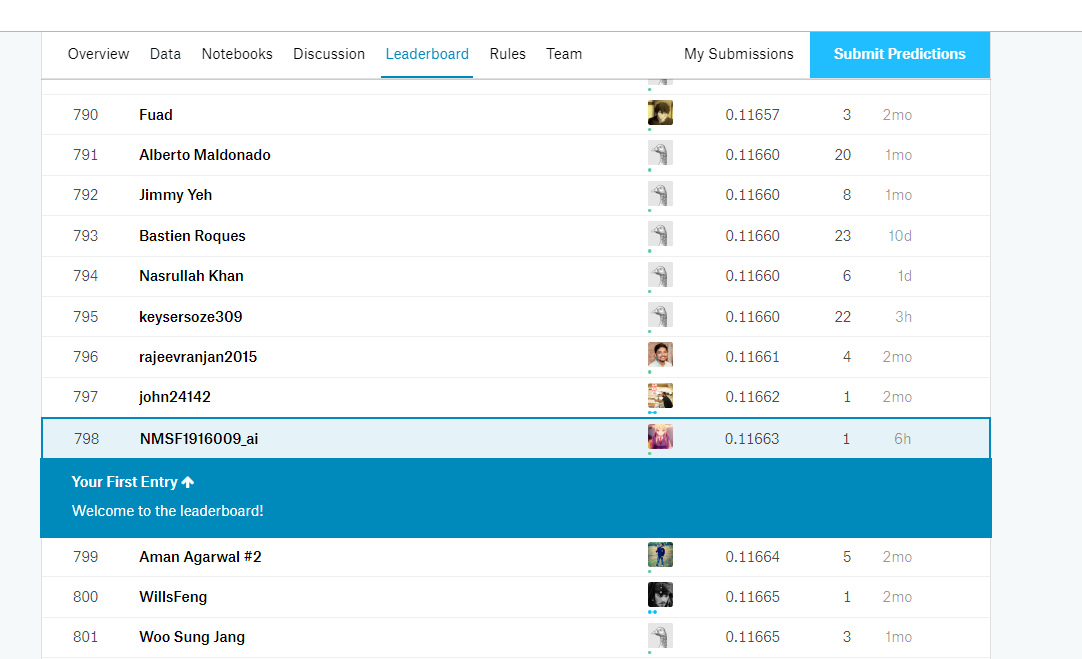
\includegraphics[width=0.8\linewidth]{figure/deta}
	\caption[比赛排名]{}
	\label{fig:deta}
\end{figure}
Score:0.11663 \\
ID:NMSF1916009\_ai \\
Rank:798
\newpage
\begin{thebibliography}{9}
	\addcontentsline{toc}{section}{参考文献}
	
	% \printbibliography[heading=bibliography,title=参考文献]
	
	% 每条参考文献均需用<\bibitem{}>引出,
	% 花括号里的内容为此条参考文献的标签,
	% 可用<\cite{}>引用。
	% 若参考文献条数超过99,
	% 请联系作者修改.cls类文件,
	% 否则空格略有不完美。
	\bibitem{bibc1}dpwang.windows下使用conda安装xgboost问题-[EB/OL][2019–12–14].https://blog.csdn.net/dpengwang/article/details/89433034.
	
	\bibitem{bibc2} 佚名. Stacking算法[EB/OL]([2019–12–15]. https://www.jianshu.com/p/59313f43916f.
	
	\bibitem{bibc3}  01编程之路.sklearn库中数据预处理函数fit\_transform()和transform()的区别[EB/OL][2019–12–14].https://blog.csdn.net/qq\_30638831/article/details/80200684.
	
	\bibitem{bibc4} LeatherWang的博客.QQ图判断一个分布是否为正态分布[EB/OL][2019–12–15].https://blog.csdn.net/hzwwpgmwy/article/details/79178485.
	\bibitem{bibc5}  打江南走过一阵. 《numpy.ndarray》 object has no attribute《values》-[EB/OL][2019–12–15].https://blog.csdn.net/FYZ530357172/article/details/73188039.
	\bibitem{bibc6}去向前方的博客.Anaconda:包安装以XGBoost为例[EB/OL][2019–12–14].https://blog.csdn.net/lvsehaiyang1993/article/details/80619495.
	\bibitem{bibc7}素质云笔记.结构化数据转换方式之一:box-cox转换[EB/OL][2019–12–15].https://blog.csdn.net/sinat\_26917383/article/details/77864582.
	
	\bibitem{bibc8} 佚名.从0到1走进Kaggle[EB/OL][2019–12–15].https://zhuanlan.zhihu.com/p/61660061.
	\bibitem{bibc9} COCK D, DEAN. Ames, iowa: alternative to the boston housing data as an end of semester regression project[J]. Journal of Statistics Education, 19(3): 8.
\end{thebibliography}

\end{document} 
%\bibliography{opt}
%\printbibliography[heading=bibliography,title=参考文献]

